\documentclass[oneside,authoryear,spanish,a4paper]{ezthesis}
%\documentclass[oneside,authoryear,draft,spanish]{ezthesis}
%\documentclass[oneside,authoryear,draftmarks,spanish]{ezthesis}
%% # Opciones disponibles para el documento #
%%
%% Las opciones con un (*) son las opciones predeterminadas.
%%
%% Modo de compilar:
%%   draft            - borrador con marcas de fecha y sin im'agenes
%%   draftmarks       - borrador con marcas de fecha y con im'agenes
%%   final (*)        - version final de la tesis
%%
%% Tama'no de papel:
%%   letterpaper (*)  - tama'no carta (Am'erica)
%%   a4paper          - tama'no A4    (Europa)
%%
%% Formato de impresi'on:
%%   oneside          - hojas impresas por un solo lado
%%   twoside (*)      - hijas impresas por ambos lados
%%
%% Tama'no de letra:
%%   10pt, 11pt, o 12pt (*)
%%
%% Espaciado entre renglones:
%%   singlespace      - espacio sencillo
%%   onehalfspace (*) - espacio de 1.5
%%   doublespace      - a doble espacio
%%
%% Formato de las referencias bibliogr'aficas:
%%   numbers          - numeradas, p.e. [1]
%%   authoryear (*)   - por autor y a'no, p.e. (Newton, 1997)
%%
%% Opciones adicionales:
%%   spanish         - tesis escrita en espa'nol
%%
%% Desactivar opciones especiales:
%%   nobibtoc   - no incluir la bibiolgraf'ia en el 'Indice general
%%   nofancyhdr - no incluir "fancyhdr" para producir los encabezados
%%   nocolors   - no incluir "xcolor" para producir ligas con colores
%%   nographicx - no incluir "graphicx" para insertar gr'aficos
%%   nonatbib   - no incluir "natbib" para administrar la bibliograf'ia

%% Paquetes adicionales requeridos se pueden agregar tambi'en aqu'i.
%% Por ejemplo:
\usepackage{etex}
\usepackage[caption=false]{subfig}
\usepackage{multirow}
\usepackage[activeacute,spanish]{babel}
\usepackage[utf8]{inputenc}
\usepackage{amsmath}
\usepackage{mathtools}
\usepackage{amsmath,amssymb,amsfonts,latexsym,cancel}
\usepackage{rawfonts}
\usepackage{pictexwd}
\usepackage{float}
\usepackage{mdwlist}
\usepackage{booktabs}
\usepackage{graphicx}
\numberwithin{equation}{section}
%paquete para diagramas
\usepackage[all]{xy}
\usepackage{mathrsfs}
%\usepackage{tikz}
%\usetikzlibrary{3d}
%\usepackage{tikz-3dplot}
\usepackage[thinlines]{easytable}
\usepackage[none]{hyphenat}
%Configuracion codigo c++
\usepackage{listings}
\usepackage[T1]{fontenc}
\usepackage{times}
\usepackage{color}
\usepackage{units}
\definecolor{lightblue}{rgb}{0, 0.7, .7}
\definecolor{gray97}{gray}{.97}
\definecolor{gray75}{gray}{.75}
\definecolor{gray45}{gray}{.45}
\lstset{ frame=Ltb,
framerule=0pt,
aboveskip=0.5cm,
framextopmargin=3pt,
framexbottommargin=3pt,
framexleftmargin=0.4cm,
framesep=0pt,
rulesep=.4pt,
backgroundcolor=\color{gray97},
rulesepcolor=\color{black},
%
stringstyle=\ttfamily,
showstringspaces = false,
basicstyle=\tiny\ttfamily,
commentstyle=\color{gray45},
keywordstyle=\bfseries,
%
numbers=left,
numbersep=15pt,
numberstyle=\tiny,
numberfirstline = false,
breaklines=true,
}
% minimizar fragmentado de listados
\lstnewenvironment{listing}[1][]
{\lstset{#1}\pagebreak[0]}{\pagebreak[0]}

\lstdefinestyle{consola}
{basicstyle=\scriptsize\bf\ttfamily,
backgroundcolor=\color{gray75},
}

\lstdefinestyle{C}
{language=C,
}

\lstdefinestyle{customc}{
  belowcaptionskip=1\baselineskip,
  breaklines=true,
  frame=L,
  xleftmargin=\parindent,
  language=C,
  showstringspaces=false,
  basicstyle=\footnotesize\ttfamily,
  keywordstyle=\bfseries\color{green!40!black},
  commentstyle=\itshape\color{purple!40!black},
  identifierstyle=\color{blue},
  stringstyle=\color{orange},
}

\lstdefinestyle{customasm}{
  belowcaptionskip=1\baselineskip,
  frame=L,
  xleftmargin=\parindent,
  language=[x86masm]Assembler,
  basicstyle=\footnotesize\ttfamily,
  commentstyle=\itshape\color{purple!40!black},
}

\lstset{escapechar=@,style=customc,basicstyle=\small}
%



%%##################################################################################################################################
%% # Datos del documento #
%% Nota que los acentos se deben escribir: \'a, \'e, \'i, etc.
%% La letra n con tilde es: \~n.

\author{Sebastián Orlando Cueto del Fierro}

\title{``ESTUDIO EXPERIMENTAL DEL COMPORTAMIENTO DE FATIGA PARA EL MATERIAL ABS IMPRESO EN 3D''}
\degree{Ingeniería Mecánica Industrial }
\supervisor{Phd. Alejandro Pacheco Sanjuan}
\correferent{Dra. Sheila Lascano Farak}
\institution{UNIVERSIDAD TÉCNICA FEDERICO SANTA MARÍA}
\faculty{Escuela de Ingeniería y Ciencias}
\department{DEPARTAMENTO DE INGENIERÍA MECÁNICA}
\city{VALPARAÍSO}
\country{CHILE}

%% # M'argenes del documento #
%% 
%% Quitar el comentario en la siguiente linea para austar los m'argenes del
%% documento. Leer la documentaci'on de "geometry" para m'as informaci'on.

\geometry{top=35mm,bottom=35mm,inner=30mm,outer=30mm}

%% El siguiente comando agrega ligas activas en el documento para las
%% referencias cruzadas y citas bibliogr'aficas. Tiene que ser *la 'ultima*
%% instrucci'on antes de \begin{document}.
\hyperlinking
\begin{document}

\sloppy 


%% En esta secci'on se describe la estructura del documento de la tesis.
%% Consulta los reglamentos de tu universidad para determinar el orden
%% y la cantidad de secciones que debes de incluir.

%% # Portada de la tesis #
%%% ## Construye tu propia portada ##
%% 
%% Una portada se conforma por una secuencia de "Blocks" que incluyen
%% piezas individuales de informaci'on. Un "Block" puede incluir, por
%% ejemplo, el t'itulo del documento, una im'agen (logotipo de la universidad),
%% el nombre del autor, nombre del supervisor, u cualquier otra pieza de
%% informaci'on.
%%
%% Cada "Block" aparece centrado horizontalmente en la p'agina y,
%% verticalmente, todos los "Blocks" se distruyen de manera uniforme 
%% a lo largo de p'agina.
%%
%% Nota tambi'en que, dentro de un mismo "Block" se pueden cortar
%% lineas usando el comando \\
%%
%% El tama'no del texto dentro de un "Block" se puede modificar usando uno de
%% los comandos:
%%   \small      \LARGE
%%   \large      \huge
%%   \Large      \Huge
%%
%% Y el tipo de letra se puede modificar usando:
%%   \bfseries - negritas
%%   \itshape  - it'alicas
%%   \scshape  - small caps
%%   \slshape  - slanted
%%   \sffamily - sans serif
%%
%% Para producir plantillas generales, la informaci'on que ha sido inclu'ida
%% en el archivo principal "tesis.tex" se puede accesar aqu'i usando:
%%   \insertauthor
%%   \inserttitle
%%   \insertsupervisor
%%	 \insertcorreferent
%%   \insertinstitution
%%   \insertdegree
%%   \insertfaculty
%%   \insertdepartment
%%	 \insertcity
%%	 \insertcountry
%%   \insertsubmitdate

\begin{titlepage}
	\TitleBlock[\vspace{-1.5 in}]{
\includegraphics[height=4cm]{Imagenes/utfsm_logo}}
	\TitleBlock[\vspace{0.05in}]{\bfseries\insertinstitution}
	\TitleBlock[\vspace{0.05in}]{\insertdepartment}
	\TitleBlock[\vspace{0.05in}]{\insertcity - \insertcountry}
	\TitleBlock[\vspace{1.2in}]{\Large\scshape\bfseries\inserttitle}
    \TitleBlock[\vspace{1.5in}]{\bfseries\insertauthor}
	\TitleBlock[\vspace{0.1in}]{\insertdegree}
	\TitleBlock[\vspace{0.1in}]{Julio - \insertsubmitdate}
\end{titlepage}

%% Nota 1:
%% Se puede agregar un escudo o logotipo en un "Block" como:
%%   \TitleBlock{\includegraphics[height=4cm]{escudo_uni}}
%% y teniendo un archivo "escudo_uni.pdf", "escudo_uni.png" o "escudo_uni.jpg"
%% en alg'un lugar donde LaTeX lo pueda encontrar.

%% Nota 2:
%% Normalmente, el espacio entre "Blocks" se extiende de modo que el
%% contenido se reparte uniformemente sobre toda la p'agina. Este
%% comportamiento se puede modificar para mantener fijo, por ejemplo, el
%% espacio entre un par de "Blocks". Escribiendo:
%%   \TitleBlock{Bloque 1}
%%   \TitleBlock[\bigskip]{Bloque2}
%% se deja un espacio "grande" y de tama~no fijo entre el bloque 1 y 2.
%% Adem'as de \bigskip est'an tambi'en \smallskip y \medskip. Si necesitas
%% aun m'as control puedes usar tambi'en, por ejemplo, \vspace*{2cm}.



%%%Pagina en blanco sin numeracion
\newpage
$\ $\\
\thispagestyle{empty}
%%% ## Construye tu propia portada ##
%% 
%% Una portada se conforma por una secuencia de "Blocks" que incluyen
%% piezas individuales de informaci'on. Un "Block" puede incluir, por
%% ejemplo, el t'itulo del documento, una im'agen (logotipo de la universidad),
%% el nombre del autor, nombre del supervisor, u cualquier otra pieza de
%% informaci'on.
%%
%% Cada "Block" aparece centrado horizontalmente en la p'agina y,
%% verticalmente, todos los "Blocks" se distruyen de manera uniforme 
%% a lo largo de p'agina.
%%
%% Nota tambi'en que, dentro de un mismo "Block" se pueden cortar
%% lineas usando el comando \\
%%
%% El tama'no del texto dentro de un "Block" se puede modificar usando uno de
%% los comandos:
%%   \small      \LARGE
%%   \large      \huge
%%   \Large      \Huge
%%
%% Y el tipo de letra se puede modificar usando:
%%   \bfseries - negritas
%%   \itshape  - it'alicas
%%   \scshape  - small caps
%%   \slshape  - slanted
%%   \sffamily - sans serif
%%
%% Para producir plantillas generales, la informaci'on que ha sido inclu'ida
%% en el archivo principal "tesis.tex" se puede accesar aqu'i usando:
%%   \insertauthor
%%   \inserttitle
%%   \insertsupervisor
%%	 \insertcorreferent
%%   \insertinstitution
%%   \insertdegree
%%   \insertfaculty
%%   \insertdepartment
%%	 \insertcity
%%	 \insertcountry
%%   \insertsubmitdate

\begin{titlepage}
	\TitleBlock[\vspace{-0.05in}]{
		\bfseries\insertinstitution}
	\TitleBlock[\vspace{-0.05in}]{
		\insertdepartment}
	\TitleBlock[\vspace{-0.05in}]{
		\insertcity - \insertcountry}
	\TitleBlock[\vspace{10mm}]{
		
\includegraphics[height=4cm]{Imagenes/utfsm_logo}}
	\TitleBlock[\vspace{0.5in}]{
		\small\scshape\bfseries\inserttitle}
	\TitleBlock[\vspace{0.5in}]{
		\small\scshape\bfseries\insertauthor}
    \TitleBlock[\vspace{0.5in}]{
    	Memoria de Títulación para optar al título de \\
    	 \insertdegree}
		\begin{minipage}{0.99\textwidth}
			\TitleBlock[\vspace{0.5in}]{
				\begin{center}
					Profesor Guia: \insertsupervisor
				\end{center}}
			\TitleBlock{
				\begin{center}
					Profesor Correferente: \insertcorreferent
				\end{center}}
			%\TitleBlock{
			%\begin{center}
			%		Profesor Correferente externo: \insertcorreferentextern
			%\end{center}}
		\end{minipage}
		\TitleBlock{Marzo - \insertsubmitdate}
\end{titlepage}

%% Nota 1:
%% Se puede agregar un escudo o logotipo en un "Block" como:
%%   \TitleBlock{\includegraphics[height=4cm]{escudo_uni}}
%% y teniendo un archivo "escudo_uni.pdf", "escudo_uni.png" o "escudo_uni.jpg"
%% en alg'un lugar donde LaTeX lo pueda encontrar.

%% Nota 2:
%% Normalmente, el espacio entre "Blocks" se extiende de modo que el
%% contenido se reparte uniformemente sobre toda la p'agina. Este
%% comportamiento se puede modificar para mantener fijo, por ejemplo, el
%% espacio entre un par de "Blocks". Escribiendo:
%%   \TitleBlock{Bloque 1}
%%   \TitleBlock[\bigskip]{Bloque2}
%% se deja un espacio "grande" y de tama~no fijo entre el bloque 1 y 2.
%% Adem'as de \bigskip est'an tambi'en \smallskip y \medskip. Si necesitas
%% aun m'as control puedes usar tambi'en, por ejemplo, \vspace*{2cm}.



%%%Pagina en blanco sin numeracion
\newpage
$\ $\\
\thispagestyle{empty}
%%% ## Construye tu propia portada ##
%% 
%% Una portada se conforma por una secuencia de "Blocks" que incluyen
%% piezas individuales de informaci'on. Un "Block" puede incluir, por
%% ejemplo, el t'itulo del documento, una im'agen (logotipo de la universidad),
%% el nombre del autor, nombre del supervisor, u cualquier otra pieza de
%% informaci'on.
%%
%% Cada "Block" aparece centrado horizontalmente en la p'agina y,
%% verticalmente, todos los "Blocks" se distruyen de manera uniforme 
%% a lo largo de p'agina.
%%
%% Nota tambi'en que, dentro de un mismo "Block" se pueden cortar
%% lineas usando el comando \\
%%
%% El tama'no del texto dentro de un "Block" se puede modificar usando uno de
%% los comandos:
%%   \small      \LARGE
%%   \large      \huge
%%   \Large      \Huge
%%
%% Y el tipo de letra se puede modificar usando:
%%   \bfseries - negritas
%%   \itshape  - it'alicas
%%   \scshape  - small caps
%%   \slshape  - slanted
%%   \sffamily - sans serif
%%
%% Para producir plantillas generales, la informaci'on que ha sido inclu'ida
%% en el archivo principal "tesis.tex" se puede accesar aqu'i usando:
%%   \insertauthor
%%   \inserttitle
%%   \insertsupervisor
%%	 \insertcorreferent
%%   \insertinstitution
%%   \insertdegree
%%   \insertfaculty
%%   \insertdepartment
%%	 \insertcity
%%	 \insertcountry
%%   \insertsubmitdate

\begin{titlepage}
	\TitleBlock[\vspace{-1.50in}]{
		\begin{flushleft}
			\small \scshape TITULO DE LA TESIS:
		\end{flushleft}
		}
	\TitleBlock[\vspace{0.00in}]{
		\small \textbf{\inserttitle}
		}
	\TitleBlock[\vspace{0.00in}]{
		\begin{flushleft}
			\small AUTOR:
		\end{flushleft}
		}
	\TitleBlock[\vspace{0.0in}]{
		\textbf{\insertauthor}
		}
    \TitleBlock[\vspace{1.0in}]{
    	\small TRABAJO DE TESIS, presentado en cumplimiento parcial de los requisitos para el Grado de \insertdegree de la Universidad T\'ecnica Federico Santa Mar\'ia.
		}
	\begin{minipage}{0.45\textwidth}
		\TitleBlock[\vspace{1in}]{
			\begin{center}
				\small \insertsupervisor
			\end{center}
			}
		\TitleBlock[\vspace{0.3in}]{
			\begin{center}
				\small \insertcorreferent
			\end{center}
			}
	\end{minipage}
	\begin{minipage}{0.45\textwidth}
%		\begin{figure}[H]
%			\centering
%			\vspace{0.7in}
%			\includegraphics[width=0.5\linewidth]{../firma_gers.png}
%		\end{figure}
%		\begin{figure}[H]
%			\centering
%			\vspace{-0.5in}
%			\includegraphics[width=0.5\linewidth]{../firma_olivier.png}
%		\end{figure}
%		\begin{figure}[H]
%			\centering
%			\vspace{-0.3in}
%			\includegraphics[width=0.7\linewidth]{../firma_elicer.png}
%		\end{figure}
		
				\TitleBlock[\vspace{1in}]{
					\begin{center}
						\small .............................
					\end{center}
					}
				\TitleBlock[\vspace{0.3in}]{
					\begin{center}
						\small .............................
					\end{center}
					}
	\end{minipage}
	\TitleBlock[\vspace{1.5in}]{
		\\
		\small \insertcity , \insertcountry - \insertsubmitdate		
		}
\end{titlepage}

%% Nota 1:
%% Se puede agregar un escudo o logotipo en un "Block" como:
%%   \TitleBlock{\includegraphics[height=4cm]{escudo_uni}}
%% y teniendo un archivo "escudo_uni.pdf", "escudo_uni.png" o "escudo_uni.jpg"
%% en alg'un lugar donde LaTeX lo pueda encontrar.

%% Nota 2:
%% Normalmente, el espacio entre "Blocks" se extiende de modo que el
%% contenido se reparte uniformemente sobre toda la p'agina. Este
%% comportamiento se puede modificar para mantener fijo, por ejemplo, el
%% espacio entre un par de "Blocks". Escribiendo:
%%   \TitleBlock{Bloque 1}
%%   \TitleBlock[\bigskip]{Bloque2}
%% se deja un espacio "grande" y de tama~no fijo entre el bloque 1 y 2.
%% Adem'as de \bigskip est'an tambi'en \smallskip y \medskip. Si necesitas
%% aun m'as control puedes usar tambi'en, por ejemplo, \vspace*{2cm}.


%% # Prefacios #
%% Por cada prefacio (p.e. agradecimientos, resumen, etc.) crear
%% un nuevo archivo e incluirlo aqu'i.
%% Para m'as detalles y un ejemplo mirar el archivo "gracias.tex".
%\thispagestyle{empty}
\vspace*{\fill}
\begin{quote}
	\raggedleft
	\emph{The more we learn about the world, and the deeper our learning, the more conscious, specific, and articulate will be our knowledge of what we do not know, our knowledge of our ignorance. For this, indeed, is the main source of our ignorance — the fact that our knowledge can be only finite, while our ignorance must necessarily be infinite}
	
	\bigskip
	\emph{Karl Popper}
\end{quote}
\vspace*{\fill}



%%% Las secciones del "prefacio" inician con el comando \prefacesection{T'itulo}
%% Este tipo de secciones *no* van numeradas, pero s'i aparecen en el 'indice.
%%
%% Si quieres agregar una secci'on que no vaya n'umerada y que *tampoco*
%% aparesca en el 'indice, usa entonces el comando \chapter*{T'itulo}
%%
%% Recuerda que aqu'i ya puedes escribir acentos como: 'a, 'e, 'i, etc.
%% La letra n con tilde es: 'n.

\prefacesection{Agradecimientos}
Es difícil escribir y sintetizar en un par de párrafos los agradecimientos a un grupo de personas que han aparecido a lo largo de estos 8 años. Mis agradecimientos van principalmente hacia aquellas personas que me han marcado profundamente en este proceso, pero también hacia aquellas personas que de alguna o otra forma incidieron en mi paso por la universidad, incluso a aquellos que no conocí ni saludé. Son estos dos conjuntos de personas quienes agradezco por ser parte de este devenir, quienes en algún punto influyeron en mis tiempos, mis decisiones y todo aquello sobre lo que no tuve control, pero que finalmente, se acoplaron para poder dar cierre a este ciclo de mi vida.

Quiero agradecer a mi familia, a mi mamá y papá por apoyarme durante toda esta etapa, por permitirme el privilegio de dedicarme exclusivamente a los estudios y a otras cosas, inclusive. Por brindarme todas las herramientas necesarias, desde que nací hasta hoy, entregándome su tiempo, disposición y amor sin esperar retribución alguna, por retarme y alentarme cuando fuese necesario, pero por sobretodo por creer en mí y en mis capacidades. A mi abuela Rosa y mi abuelo Hernán, quienes llegaron a ser unos segundos padres al consintirme, formarme e impregnarme de su amor por los libros, la música, los relatos y su cariño.

Por otro lado, también agradezco a mi amiga Susi, a mis amigos Patricio, Marcelo, Pablo Campos, Pablo Kohler, Cristián, Sebastián y Pablo Cárdenas, quienes conozco desde mis primeros años en la universidad o antes, que me apoyaron en los momentos difíciles y me felicitaron en los momentos alegres. Les agradezco su capacidad de discusión, de poder opinar libremente y la idea de siempre buscar construirnos como mejores personas, por su infaltable cariño y afecto que hizo más ameno mi paso por la universidad, en especial a los tres últimos quienes me ayudaron a desarrollar esta tesis con sus conocimientos y el abrirse a escucharme. Por otro lado, quiero agradecer a Laura, quien fue mi amiga y compañera, por su inconmensurable amor, dedicación y paciencia, por su capacidad de creer en mí, aún en los momentos más oscuros. No fueron sino las risas, la compañía y su sabiduría lo que me permitieron llegar hasta donde estoy.

A mis compañeros de banda, con quienes durante 8 años ensayamos, compartimos y nos enseñamos al rededor de la música. La excusa de juntarse a tocar instrumentos de forma coordinada desencadenó en una amistad y un espacio de aprendizaje profundo que sobrepasa las dimensiones de la banda misma. Sin duda, cada ensayo y cada creación fueron un escape de la universidad, permitiéndonos dialogar y expresarnos a través de nuestra música, pero también al abrirnos y exponer nuestros sentimientos en la conversación.

Finalmente, al profesor Alejandro Pacheco, con quien tuve la suerte de desarrollar esta tesis, contar con su apoyo e infinita paciencia. La dedicación que tuvo al destinar de su tiempo para enseñarme, responder mis dudas y corregirme cada vez que me equivocaba fueron una constante luz en este largo proceso.  Sin duda su empuje a estudiar, comprender y aplicar lo aprendido me dejo una marca importante en mi formación que espero lograr plasmar en mi futuro como ingeniero. 

%%%Pagina en blanco sin numeracion
\newpage
$\ $\\
\thispagestyle{empty}
%%% Las secciones del "prefacio" inician con el comando \prefacesection{T'itulo}
%% Este tipo de secciones *no* van numeradas, pero s'i aparecen en el 'indice.
%%
%% Si quieres agregar una secci'on que no vaya n'umerada y que *tampoco*
%% aparesca en el 'indice, usa entonces el comando \chapter*{T'itulo}
%%
%% Recuerda que aqu'i ya puedes escribir acentos como: 'a, 'e, 'i, etc.
%% La letra n con tilde es: 'n.
\prefacesection{Abstract}


%%%Pagina en blanco sin numeracion
\newpage
$\ $\\
\thispagestyle{empty}
%\prefacesection{Resumen}

El desarrollo de este trabajo se encuentra entorno a la máquina de fatiga en flexión del laboratorio de tecnología mecánica, el cual tiene como objetivo avanzar hacia la operatividad de la máquina. Para esto, la metodología se dividió en 4 etapas: levantamiento de información, diseño de una estructura soportante, modelar el comportamiento de la máquina y contrastar los resultados con la información existente.

La máquina tiene problemas en su funcionamiento, mantenibilidad y disponibilidad de respuestos producto de su antigüedad. Su funcionamiento se basa en una tabla de cargas (anexo \ref{sec:anexob1}), que relaciona los contrapesos con los esfuerzos sobre probeta.

El diseño de la estructura se realizó de acero y madera, utilizando como guía la norma NCh 1198. Además, a través de MEF se simuló el comportamiento estático y modal de la estructura. De esta manera, la dimensión final de cada componente se exponen en los planos del anexo \ref{sec:planos}.

Para el modelamiento de la máquina, se utilizaron los datos obtenidos en el levantamiento de información y se resolvieron las ecuaciones de movimiento utilizando el método de energía. Así, se obtuvo el movimiento y la velocidad del centro de masa del brazo de carga. A través de esto, se calculó la fuerza realizada sobre la probeta para distintas configuraciones. La carga máxima posible, según el modelo, es de $1498.83$ [N], a una velocidad de rotación del disco $\omega_{max} =$ 25 [rad/s]. 

Estos resultados de fuerza máxima se simularon usando MEF, utilizando como límite el esfuerzo último del material. Por lo tanto, se obtuvo una nueva relación entre las combinaciones de los contrapesos y los esfuerzos en la probeta, las cuales se muestran en la propuesta \ref{sec:anexob2}.  

Con la información y los resultados obtenidos, se puede concluir que es necesaria una actualización y reparación de la máquina de fatiga, como también la construcción de la estructura para lograr que la máquina este operativa. Además existen discrepancias entre el modelo propuesto y la información existente, ante lo cual es necesario hacer un trabajo posterior que valide, refute o corrija el modelo y la tabla de cargas propuesta. 

%El desarrollo de este trabajo se encuentra entorno a la máquina de fatiga en flexión del laboratorio de tecnología mecánica, en Valparaíso. Actualmente no se encuentra operativa, por lo tanto, el objetivo de este trabajo es avanzar en la dirección que permita volver a tener operativa la máquina. Para esto, la metodología de trabajo se dividió en 4 grandes etapas: levantamiento de información, diseño de una estructura soportante para su anclaje, modelar el comportamiento de la máquina y, finalmente, contrastar los resultados con la información existente de la máquina.
%
%Esta máquina tiene una antigüedad que ronda los 60 años, lo que implica varios problemas para su mantenimiento y reparación. Diversos componentes se encuentran en desuso, alguna tecnologías están obsoletas y la información respecto a la máquina es escasa. Es por esto, que se hace necesario conocer el funcionamiento de la máquina, diseñar una nueva estructura y actualizar sus componentes. El funcionamiento actual de la máquina se basa en una tabla de carga, que relaciona la combinación de contrapesos con los esfuerzos que sufrirá la probeta a ensayar.
%
%El diseño de la estructura se realizó de acero y madera, con uniones mecánicas entre cada elemento. Para los cálculos en madera, se utiliza como guía la norma NCh 1198, la cual entrega toda la metodología de cálculo necesaria. Además, a través de elementos finitos, mediante el software Inventor, se simuló el comportamiento estático y modal. Los resultados se exponen en los planos de la estructura en el anexo \ref{sec:planos}, tanto para las dimensiones de la madera, el acero y sus uniones respectivas.
%
%Para el modelamiento del movimiento de los componentes de la máquina, se utilizaron los datos obtenidos en el levantamiento de información y se resolvieron las ecuaciones de movimiento  a través del método de energía. Así, se obtuvo el movimiento y la velocidad lineal y angular del brazo de carga respecto a su centro de masa, con lo cual fue posible calcular la fuerza realizada sobre la probeta para distintas configuraciones de contrapesos. La carga media obtenida es de $12.438$ [N] y la carga máxima posible es de $1498.83$ [N], ambas a una velocidad de rotación del disco $\omega_{max} =$ 25 [rad/s]. 
%
%Estos resultados de fuerza máxima, se simularon en elementos finitos, mediante el software ANSYS, todas las cargas hasta que la probeta alcanzó su esfuerzo último. Por lo tanto, se obtuvo una relación entre las combinaciones de los contrapesos y los esfuerzos en la probeta asociados a cada configuración, las cuales se pueden ver en la tabla de cargas propuesta, en el anexo \ref{sec:anexob2}.  
%
%Con la información y los resultados obtenidos, se puede concluir que es necesaria una actualización y reparación de la máquina de fatiga, como también la construcción de la estructura para lograr que la máquina este operativa. Además existen discrepancias entre el modelo propuesto y la información existente, ante lo cual es necesario hacer un trabajo posterior que valide, refute o corrija el modelo y la tabla de cargas propuesta.
%%%Pagina en blanco sin numeracion
\newpage
$\ $\\
\thispagestyle{empty}

%%% # 'Indices y listas de contenido #
%%% Quitar los comentarios en las lineas siguientes para obtener listas de
%%% figuras y cuadros/tablas.

%%%% Indice
\tableofcontents
%%%% Indice de figuras
\listoffigures
%%%% Indice de tablas
\listoftables

%
%%% # Cap'itulos #
%%% Por cada cap'itulo hay que crear un nuevo archivo e incluirlo aqu'i.
%%% Mirar el archivo "intro.tex" para un ejemplo y recomendaciones para
%%% escribir.
%
%\chapter{Introducción}

Las prótesis y la impresion 3D son tópicos que han ido tomando importancia durante la última década. La impresión 3D, como tecnología, ha crecido fuertemente desde la aparición de las impresoras de escritorio, las cuales permiten a cualquier persona sin conocimientos específicos de ingeniería, poder imprimir piezas u objetos diseñados por el propio usuario sin tener que contar con equipo especializado. Un ejemplo de este rápido crecimiento se puede notar en una noticia del periódico The Economist de hace más de una década: 

\begin{quote}
\textit{If you really want to impress your friends with high-tech wizardry in 2008 then consider shopping for a three-dimensional printer. (``A Whole New Dimension'', 2007)}
\end{quote}


Esta transición de una tecnología restringida a la industria especializada hacia lo privado o industrias de pequeña escala, llevó a un desarrollo y aplicación de la impresión 3D más disgregada, independiente de las principales marcas fabricantes de impresoras, permitiendo el surgimiento de comunidades, startups o incluso iniciativas universitarias centradas en la investigación o desarrollo de aplicaciones y mejoras de esta tecnología. Como consecuencia de esto, se crearon nuevas marcas de impresión 3D como MakerBot, surgieron comunidades de libre acceso como RepRap y también diversas iniciativas desarrollaron prótesis, principalmente de brazo, impresas en 3D.

Por otro lado, las prótesis de extremidades que actualmente se comercializan tienen un costo que es muy superior al que pueden pagar los potenciales usuarios, el cual se ve encarecido a medida que los diseños son más versátiles y para algún requerimiento específico, como el atletismo o el ciclismo. Además, estas necesitan de una infraestructura de salud que de apoyo en el uso y mantenimiento de las prótesis, restringiendo su aplicación a zonas con un alto desarrollo hospitalario \cite{vujaklija20183d}. Dado que se espera que las amputaciones de extremidades inferiores aumenten considerablemente en las próximas décadas, se vuelve necesario buscar alternativas y soluciones para las problemáticas de las prótesis tradicionales, buscando mejorar la calidad de vida de los pacientes \cite{franchignoni2015rasch}.

Así, las prótesis fabricadas con impresión 3D surgen como una solución para estas problemáticas. De esta forma, distintos diseños, desarrollos y alternativas surgen desde distintos lugares y con objetivos distintos. Por un lado, existe un desarrollo de libre acceso destinado a solucionar de manera rápida y autónoma las problemáticas de las personas con discapacidad motora, buscando que cada usuario pueda modificar e imprimir sus prótesis. Y por otro, empresas han buscado crear o mejorar diseños existentes con el objetivo de poder entregar un producto que se adapte mejor a cada paciente y situación, sin los grandes costos que implica la compra de una prótesis tradicional.

Dependiendo del tipo de prótesis, estarán sometidas a distintas cargas estáticas y fluctuantes y tendrán un uso más reiterativo o puntual. En consecuencia, surge la necesidad de tener información respecto al comportamiento mecánico del material manufacturado bajo condiciones específicas como lo es la impresión 3D por deposición fundida (FDM, por sus siglas en inglés). Para el plástico ABS, existen distintos estudios respecto a sus propiedades a tensión y compresión bajo distintas configuraciones de carácter estático, sin embargo, la información disponible sobre su comportamiento bajo cargas dinámicas es bastante escasa \cite{lee2013fatigue}\cite{zhang2018tensile}, dificultando la predicción de su vida útil y, a su vez, la confiabilidad que tendrá durante su uso.

Así, las cargas variables generan un daño en las estructuras al provocar micro-grietas que se expanden con cada ciclo de carga y que reducen las propiedades mecánicas del material. Este daño provocado por una o varias cargas variables y repetitivas en el tiempo es llamada fatiga y la resistencia a la fatiga es la capacidad de un material de soportar este daño. Para estudiar las propiedades de un material o elemento frente a la fatiga, se deben realizar ensayos que logren dar información relevante para los casos de estudio, como en este caso son las prótesis, existiendo distintas tipos de máquinas, normas y tecnologías que se adaptan a las distintas necesidades.

De este modo, este trabajo se enmarca en el proyecto de análisis de una prótesis transtibial fabricada a través de FDM con material ABS. Con este proyecto se busca conocer el comportamiento mecánico de la prótesis bajo cargas estáticas y fluctuantes, como lo son el estar de pie y caminar, para predecir la vida útil del diseño. No obstante, como se señaló anteriormente, la información existente sobre las propiedades de fatiga del material son bastante escasas, lo que nos lleva a la necesidad de generar información útil que pueda servir como datos de entrada a las simulaciones computacionales de la prótesis.

Bajo este contexto es que el presente trabajo de título busca diseñar las condiciones necesarias para la puesta en marcha de la máquina de fatiga a flexión existente en el laboratorio de tecnología mecánica del departamento de ingeniería mecánica en el campus Casa Central. Para esto, se hará un nuevo diseño para la estructura soportante que logre anclar la máquina y resistir su operación. Además se levantará información respecto a su funcionamiento, para posteriormente realizar un modelo que busque describir y predecir el movimiento de la máquina y sus componentes para comprender la carga a la que se somete la probeta. Se verificarán las cargas obtenidas simulando mediante un software de elementos finitos los esfuerzos asociados a cada configuración de la máquina, para contrastar los datos conseguidos con la información existente previamente en el laboratorio. Asimismo, se comprobará la vida a fatiga estimada con los esfuerzos obtenidos. Por último, se buscará la carga necesaria para alcanzar el esfuerzo de fluencia y último de la probeta de acero como información de referencia.

El trabajo realizado se dividirá en 4 grandes secciones a lo largo de toda esta memoria. El primero corresponde al levantamiento de información, el segundo al diseño de la estructura soportante, seguido del desarrollo del modelo vibratorio de la máquina de fatiga, para culminar en la simulación elasto-plástica de la probeta. Así, cada capítulo está compuesto por cada una de estas 4 secciones.

De esta manera, en el capítulo 2, antecedentes, se hace una breve introducción a la fatiga, las formas que existen para medirla y como se correlacionan  las distintas metodologías de medición. Luego, se habla brevemente del historial de la máquina de fatiga. Por otra parte, se pasa a caracterizar los dos materiales utilizados en este trabajo, la madera y el acero, para terminar con un esbozo de los software de elementos finitos utilizados.

A continuación, se muestra y desarrolla todo el marco teórico que apoya y sustenta el trabajo a través del capítulo 3. Se profundiza qué es la fatiga, se exponen las ecuaciones de movimiento y energía de un sistema dinámico, seguido por la derivación del método de Lagrange. Además, se expone sobre qué es la plasticidad, las relaciones de esfuerzo y deformación real y el endurecimiento por deformación isotrópico. Por último, se explica el método de elementos finitos, se deriva la ecuación de momentum lineal y se exponen las ecuaciones de esfuerzos y deformación asociadas a elementos finitos.

El capítulo 4, metodología, detalla el procedimiento con el que se llevó a cabo el trabajo. El levantamiento de información de la máquina de fatiga, la medición y descripción de sus componentes. El diseño de la estructura, los cálculos en acero, madera y sus respectivas uniones, para las cuales se utilizaron la norma NCh 1198, sintetizada en el anexo \ref{ch:anexo_a}. La derivación de las ecuaciones de movimiento para el brazo de carga y su resolución. Para terminar con la simulación, en el software ANSYS, de la probeta sometida a distintas cargas y la vida a fatiga esperada para cada combinación de contrapesos.

En el capítulo 5, se exponen los resultados obtenidos y se realiza un análisis de esta información, como también se bosquejan las primeras conclusiones del trabajo. A lo largo de este capítulo se muestran las dimensiones de cada elemento seleccionado en el caso del diseño, los datos del movimiento del brazo de carga y los esfuerzos en la probeta obtenidos por medio de la simulación, a partir de los cuales se estimó la vida a fatiga de la probeta para cada carga.

En el capítulo 6 se presentan las conclusiones a las que se llegaron producto de los resultados y la información recopilada. Para terminar, se expondrá el trabajo futuro que se abre como consecuencia de esta tesis.





%
%\chapter{Estado del Arte}
	
%
%\chapter{Marco Teórico}

\section{Fatiga}
El fenómeno en el cual una estructura se daña e incluso falla por cargas fluctuantes, es llamado fatiga. El estudio de este problema comenzó tempranamente en europa durante la mitad del siglo XIX, en pleno auge de la industralización europea, producto de la falla repentina de algunos componentes en máquinas y los ejes de los trenes de la época. Estos experimentaban un gradual debilitamiento de la resistencia, fallando aún cuando su esfuerzo último no fuese alcanzado. 

Así, en 1837 fueron publicados los resultados del primer ensayo de fatiga, realizado a una cadena transportadora utilizada en minas de hierro en Alemania. Wilhelm Albert, quien realizó esta investigación, se vió motivado a realizar los estudios por los altos costos que significaba la falla de este componente producto las cargas cílicas a las que estaba sometida. Los pocos conocimientos existentes del fenómeno, llevo a que la solución al problema fuese la invención del cable de acero.

Por otro lado, las primeras investigaciones enfocadas a comprender el fenómeno comenzaron en 1858 con August Wölher. Su acucioso estudio lo llevó a conclusiones que siguen teniendo importancia y validez hasta el día de hoy. Diseñó, durante la década de 1860, una máquina de ensayos de flexión y flexión rotativa. En 1870 presentó un informe en el cual parte de sus conclusiones cualitativas son llamadas ``Ley de Wöhler'', al establecer el esfuerzo alternante como el parámetro más importante para la vida de un componente, señalanado que ``the stress amplitudes are decisives for the destruction of the cohesion of the material. The maximum stress is of influence only in so far as the higher it is, the lower are the stress amplitudes which lead to failure''\textcolor{red}{citar schutz history of fatigue}, aunque destacando también que el esfuerzo medio tiene una influencia perjudicial en el material. 

Es decir, desde 1853 hasta hoy, han transcurrido más de 160 años de investigación sobre la fatiga, logrando comprender distintas aristas del fenómeno, pero con muchas preguntas aún sin resolver. Por eso, la fatiga sigue siendo un problema necesario de abordar y seguir comprendiendo, por sus grandes implicaciones de costo que tiene en la industria y en distintos elementos que utilizamos en la vida diaria. Por otro lado, si bien muchas preguntas no han sido resueltas científicamente, diversas empresas han logrado evitar las fallas por fatiga y optimizar los diseños de manera operativa, sin comprender cabalmente el trasfondo de estos.  



\subsection{Definiciones}
La fatiga se puede definir, desde la perspectiva del material, como el proceso en el cual el daño se acumula producto de la aplicación de cargas repetitivas que se encuentran bajo el punto de fluencia. En metales, este proceso se divide en tres fases o etapas los cuales, dependiendo del autor, pueden ser llamados: fase de iniciación de la grieta, fase de crecimiento de la grieta y fractura.

La primera fase es el inicio de una o más microgrietas, la cual ocurre tempranamente en la vida a fatiga de un material y que, incluso, pueden ocurrir inmediatamente si el esfuerzo cíclico se encuentra sobre el límite de fatiga. Lo característico de esta etapa es que las grietas no pueden verse a simple vista, fase que representa una parte considerable de la vida a fatiga total. Estas crecerán lentamente y de manera errática, debido al efecto de las microestructuras como los bordes de grano. Durante este período, las concentraciones de esfuerzo juegan un importante papel, al ser los lugares donde comenzará la nucleación de las grieta, sumado a las pocas restricciones de deslizamiento de la superficie del material, hace que esta sea relevante en el inicio de este proceso.

En la segunda etapa, las microgrietas pasan a ser macrogrietas, es decir, son visibles al ojo humano. Estas grietas comienzan a tomar una dirección de crecimiento que es perpendicular a los esfuerzos principales producidos por la carga alternante. La resistencia al crecimiento de las grietas, cuando esta penetra el material, dependerá de las propiedades de grano. Así, se puede definir cualitativamente una separación entre ambas etapas, donde el periodo de iniciación o nucleación de las grietas termina cuando su crecimiento no es dependiente de las condiciones superficiales del material. Producto de la micro-deformación plástica cíclica se forman bandas de crecimiento conocidos como \textit{marcas de playa} o \textit{``striations patterns''}, abriendo, cerrandose y frotandose entre sí, como se puede ver en la imagen \textcolor{red}{Añadir figura 2.24 de Fatigueofstructuresandmaterial 2009}, dejando en evidencia el frente de grieta, las variaciones en la carga, su velocidad de crecimiento y la naturaleza corrosiva del entorno.

Finalmente, la última etapa es la falla del material, que ocurre en el último ciclo de la carga, al no poder soportarla con el material restante. Esta fractura es rápida y es producto de una macro-deformación plástica, pudiendo ser frágil, dúctil o una combinación de ambas.

Con esto en cuenta, es posible definir ciertos conceptos en base a las distintas etapas que experimenta un material. La vida a fatiga de un material (\textit{fatigue life}, $N_f$) es el número de ciclos aplicados a una probeta para lograr el criterio de falla \textcolor{red}{referencia a ISO 23718}. El límite de resistencia a la fatiga (\textit{endurance limit}) es frecuentemente explicado como la amplitud de esfuerzo para el cual la vida a fatiga tiende a infinito o a la asíntota de la curva S-N. Sin embargo, al comprender la fatiga como un proceso, es posible dar una definición más acertada para el límite a la fatiga, pasando a ser el umbral para el crecimiento de las microgrietas. Es decir, bajo este límite existe nucleación e iniciación de grites, sin embargo, su crecimiento está limitado a los bordes de grano del material.

Por otra parte, para el estudio de este fenómeno existen tres modelos de falla por fatiga: de \textit{esfuerzo-vida} (S-N), de \textit{deformación-vida }($\epsilon$-N) y de la \textit{mecánica de fractura lineal elástica} (LEFM). Cada uno de ellos tiene ventajas y desventajas, sin embargo, la máquina que es objeto de evaluación en este trabajo utiliza el método \textit{esfuerzo-vida}. El criterio de elección entre los distintos modelos se divide principalmente por la cantidad de ciclos que se hará la medición, los que se clasifican en régimen de fatiga de ciclo bajo (\textit{low-cycle fatigue}, LCF) o un régimen de fatiga de ciclo alto (\textit{high-cycle fatigue}, HCF). La división entre ambos régimen dependerá de distintos autores, no obstante, por lo general se establece la separación en $10^3 \leq LCF$ y $10^3 > HCF$ \textcolor{red}{referencia al shigley - pag. 265}, debido a que la zona LCF está asociada a la existencia de macro-deformaciones plásticas en cada ciclo. De esta manera, el método de esfuerzo-vida se utiliza para ensayos de alto ciclaje debido a su poca precisión en casos LCF. A su vez, los métodos de deformación-vida y LEFM se aplican para casos LCF.

En el método de esfuerzo-vida las muestras o probetas son sometidas a fuerzas de magnitudes especificadas, al mismo tiempo que se cuentan la cantidad de ciclos. Es por esto que es un modelo con base en el esfuerzo, con el cual se busca determinar una resistencia de fatiga o un límite de resistencia. 

Estas fuerzas especificadas pueden ser constantes o variables en el tiempo y magnitud, sin embargo, se abordará principalmente los casos donde los esfuerzos fluctúan de manera constante en el tiempo y de una amplitud fija debido a las características de la máquina analizada en este trabajo. Esto permite trazar la curva de fatiga (S-N) del componente o material.

Se hace necesario describir y definir elementos que surgen producto de una carga cíclica. Esta se caracteriza por el esfuerzo alternante (\textit{alternate stress} o \textit{amplitude stress}, $S_a$) y el esfuerzo medio (\textit{mean stress}, $S_m$) que se muestran en la ecuación \ref{eq:s_a} y \ref{eq:s_m}, respectivamente. A su vez, estas se definen por el esfuerzo máximo $S_{max}$ y $S_{min}$, siendo el esfuerzo máximo y mínimo alcanzado por la carga cíclica. Finalmente, el rango del esfuerzo, $\Delta S$ (eq. \ref{eq:ds}), y la razón de esfuerzos, $R$ (eq. \ref{eq:r_s}), también son opciones  para caracterizar la fatiga.

\begin{align}
	S_a &= \frac{S_{max} - S_{min}}{2} \label{eq:s_a} \\
	S_m &= \frac{S_{max} + S_{min}}{2} \label{eq:s_m} \\
	\Delta S &= S_{max} - S_{min} = 2S_a  \label{eq:ds} \\
	R &= \frac{S_{min}}{S_{max}} \label{eq:r_s} 
\end{align}

Estos términos se pueden ver claramente en la figura \textcolor{red}{Insertar imagen que muestra Sa Sm etc}. Para el caso en donde $S_m = 0$, y así $R=-1$, se llama esfuerzo de ciclo invertido. Cuando $S_{min}=0$, y $R=0$, se llama esfuerzo repetido.

\subsection{Curva S-N o de Wöhler}
Como se señaló en el punto anterior, la curva S-N es el resultado de la aplicación del método esfuerzo-vida. Es quizás uno de las herramientas más importantes en el desarrollo empírico para lograr cuantificar el proceso de fatiga y poder diseñar contra este. El diagrama S-N se obtiene como resultado de un número de ensayos de fatiga a distintos niveles de esfuerzo, donde $S$ puede ser la amplitud ($S_a$), el rango de esfuerzo ($\Delta S$) o el esfuerzo máximo ($S_{max}$) que es aplicado a la probeta, siendo la amplitud lo más común. La variable $N$ hace referencia a la vida a fatiga del material, es decir, la cantidad de ciclos hasta que la probeta falle. Debido a que se desea analizar fallas en LCF y HCF, la cantidad de ciclos necesarios para fallar la probeta pueden llegar a ser demasiado altos, por esto, $N$ se grafica en escala logarítmica.

La cantidad de ensayos requeridos para construir la curva S-N dependerá de distintos factores como, por ejemplo, la confiabilidad esperada, el uso final de la información o de los recursos disponibles. La norma E739-10 -- "Statistical Analysis of Linear or Linearized Stress-Life ($S-N$) and Strain-Life ($\varepsilon -N$) Fatigue Data", establece una guía dependiendo del tipo de prueba a realizar como se muestra en al tabla \ref{tab:type_test}. Además, se recomienda realizar la medición con, al menos, tres puntos de esfuerzos distintos. Con esto, es posible obtener el diagrama $S-N$ como el que se puede apreciar en la figura \textcolor{red}{Añadir figura 6-10, Shigley, pag 266}, donde se puede apreciar la diferencia entre la zona LCF, HCF y de vida infinita, para el caso de los aceros.


\begin{table}[]
\begin{center}
\caption{Número mínimo de pruebas según tipo de prueba}
\label{tab:type_test}
\begin{tabular}{@{}lc@{}}
\toprule
\multicolumn{1}{c}{Tipo de prueba}                                                                                        & Cantidad mínima de probetas \\ \midrule
\begin{tabular}[c]{@{}l@{}}Preliminar y exploratorio (investigación exploratoria \\ y ensayos de desarrollo)\end{tabular} & 6 a 12                      \\
\begin{tabular}[c]{@{}l@{}}Pruebas de desarrollo e investigación de componentes \\ y probetas\end{tabular}                & 6 a 12                      \\
Datos de diseños permisibles                                                                                              & 12 a 24                     \\
Datos de confiabilidad                                                                                                    & 12 a 24                     \\ \bottomrule   
\end{tabular}
\end{center}
\end{table}

La curva $S-N$ varía ampliamente sus resultados para distintos tipos de materiales y, a su vez, estos se ven afectados por una variedad de factores. Estos pueden ser por modificaciones en las condiciones de ensayo, de la geometría de la probeta, de la naturaleza del material o de la forma de fabricación de la probeta. Todos estos factores crean ciertas tendencias en la obtención de datos que los distinguen unos de otros. 

En concreto, las condiciones medioambientales hostiles pueden acelerar el proceso de iniciación y crecimiento de grietas, ya sean químicas o térmicas. Una probeta sometida a creep, fatiga y altas temperaturas puede disminuir drásticamente sus vida útil y, por tanto, la vida a fatiga del material. Por otra parte, se pueden realizar ensayos en una solución de sal para homologar las condiciones marinas, afectando también su vida a fatiga. \textcolor{red}{Agregar imagen, pag. 387 y 388 - Dowling}

El esfuerzo residual también tiene incidencia en la curva de Wöhler, la cual puede incluso ser beneficiosa al utilizar técnicas como el granallado (\textit{shot peening}). El mecánizado de las piezas, como en el caso de la probeta utilizada por la máquina de fatiga, verá afectado los resultados de la curva $S-N$ dependiendo de las características con las que sea manufacturado. Como se indicó anteriormente, la primera etapa de la fatiga, la inicación de las grietas, es un fenómeno que depende de la superficie del material y como consecuencia, un mecánizado grueso o fino tendrá un impacto en esa etapa de la fatiga y no en la posterior, como se puede apreciar en la imagen \textcolor{red}{Imagen página 54 - Book of fatigue}. Así, aquellas probetas que tengan una mejor calidad superficial producto del afinado, tendrán una mejor resistencia a la fatiga respecto a otras.

Es posible encontrar otros factores que inciden en los resultados de la curva, como pueden ser la geometría de la probeta o componente, sus dimensiones, el esfuerzo último ($\sigma_{uts}$), su microestructura, tratamientos químicos y el esfuerzo medio ($S_m$). Este último será analizado en la sección siguiente, debido a la importancia que posee al estar presente en la máquina a analizar. 

%En último término, existen distintas formas de obtener la información necesario con el método esfuerzo-vida, ya sea por pruebas de fatiga axial, torsión, torsión-flexión, flexión o flexión en voladizo. Este último, es el utilizado por la máquina existente en el laboratorio de tecnología mećanica. 
%
%
%%al ser este método el más utilizado existe una gran cantidad de datos para distintos materiales, configuraciones o elementos mecánicos. Con esto resulta más fácil poder comparar resultados o encontrar información al momento de diseñar componentes que sufrirán fatiga. Por otro lado, 

\subsection{Esfuerzo medio, $S_m$}
Como se escribió anteriormente, los distintos tipos de carga aplicado en una 

\section{Norma de cálculo en madera - NCh 1198}
La norma NCh 1198 - Cálculo de construcciones en madera - estab
lece los métodos y procedimientos de diseño estructural que determinarán las condiciones mínimas que debe cumplir cada elemento de la estructura. Esta incluye las construcciones de madera aserrada, elaborada, laminada-encolada y postes de madera, como también las uniones a través de elementos mecánicos, tales como: clavos, tirafondos, pernos, barras de acero, tornillos y conectores para madera.
\subsection{Propiedades de la madera y factores de modificación}
\subsubsection{Contenido de humedad}


El contenido de humedad de una madera debe ser considerado por su susceptibilidad a los cambios de forma, volumen y para la determinación de las tensiones admisibiles debido a que es un material higroscópico. Para esto, se debe tomar en cuenta su humedad durante la construcción ($H_c$), como también, la humedad a la que estará en servicio ($H_s)$ o humedad de equilibrio. La humedad de equilibrio depende de la ubicación que tengan los elementos. Si se encuentra en un recinto cerrado sin calefacción o intermitente $H_s= 12\%$. Si es un recinto cerrado continuamente calefaccionado, entonces $H_s=9\%$. Si es un recinto cubierto abierto, entonces la humedad de equilibrio será igual a la humedad medida del lugar donde se ubicará. Finalmente, si los elementos se encuentran a la interperie, se puede utilizar la tabla que se encuentra en el anexo D, de la norma NCh 1198, para las diferentes regiones geográficas de Chile.\\

Así la \textcolor{red}{Tabla (Tabla 3 norma)} se utiliza de criterio para clasificar la madera como verde o seca, las cuales se designan con las letras E y ES, respectivamente. Además, son agrupadas con un número que agrupa las especies madereras que crecen en Chile, de acuerdo a la norma NCh 1989 - Agrupamiento de especies madereras según su resistencia - mostrada en el anexo A de la norma NCh 1198. Para el pino radiata se considera la clasificación de la norma NCh 1207 - Pino radiata, clasificación visual para uso estructural, especificaciones de los grados de calidad.\\

\textcolor{red}{COLOCAR TABLA 3}\\

\subsubsection{Densidad}
Debido a la característica higroscópica de la madera, su masa y volumen varían respecto al contenido de humedad. Por lo tanto, existen distintos tipos de densidad dependiendo de la información que sea necesaria o de los cálculos que se realicen. De acuerdo a la norma NCh 176/2, se definen los siguientes valores de densidad:
\begin{itemize}
	\item Densidad anhidra: Relaciona la masa y el volumen de la madera completamente seca (anhidra)
	\item Densidad normal: Aquella que relaciona la masa y el volumen de la madera con un contenido de humedad del 12\%.
	\item Densidad básica: Relaciona la masa anhidra de la madera y su volumen con humedad igual o superior al 30\%.
	\item Densidad nominal: Es la que relaciona la masa anhidra de la madera y su volumen con un contenido de humedad del 12\%.
	\item Densidad de referencia: Aquella que relaciona la masa y el volumen de la madera ambos con igual contenido de humedad.
\end{itemize}

\subsubsection{Tensiones admisibles y módulo de elasticidad}
La madera es un material no homogéneo constituido por fibras naturales que mantienen su dirección, las cuales inciden en que su comportamiento mecánico, su flexibilidad y la resistencia a los esfuerzos sea distinta respecto al eje en que se usa, siendo un material ortotrópico donde su resistencia es mayor en el eje paralelo a las fibras que el normal a las fibras.

Además, sus propiedades varían respecto a la especie del árbol, su edad, condiciones climáticas, humedad y la presencia de defectos, como nudos, rajaduras o agujeros. Para esto, la norma NCh 1970/1 y 1970/2 - Clasificación visual para uso estructural, especificaciones de los grados de calidad - junto a la norma NCh 1207, determinan el grado estructural desde el N$^\circ$1 al N$^\circ$4, a partir de una inspección visual de la madera procesada. Con esta clasificación, junto a la clasificación de madera seca o verde, determinan la clase estructural de la madera aserrada. Finalmente, con esta información es posible obtener la tensión admisible en flexión ($F_f$), compresión paralela a las fibras ($F_{cp}$), tracción paralela a las fibras ($F_{tp}$), cizalle ($F_{cz}$), compresión normal a las fibras ($F_{cn}$) y el módulo de elasticidad en flexión ($E_f$), de las tablas 4.a para todas las especias y 4.b para el pino radiata.

\subsubsection{Factores de modificación}
Existen otras variables externas a la madera que pueden afectar su correcto desempeño. Para esto, existen los factores de modificación que buscan corregir la tensión admisible para las distintas condiciones a las que puede estar sometido el elemento. Estas son:
\begin{itemize}
	\item Factor de modificación por contenido de humedad, $K_H$.
	\item Factor de modificación por duración de la carga, $K_D$.
	\item Factor de modificación por trabajo conjunto, $K_C$.
	\item Factor de modificación por temperatura.
	\item Factor de modificación por tratamiento químico
\end{itemize}

\subsection{Diseño de piezas}
Para el diseño de piezas es necesario calcular las tensiones de diseño, que se determinan como el producto de las tensiones admisibles por los factores de modificación que resulten pertinentes y que se definen para cada tipo de solicitación a la que está sometida cada pieza de la estructura. Por lo tanto, las tensiones de trabajo no pueden ser superiores a las de diseño, debiendo establecerse, un factor de seguridad para los cálculos. \textcolor{red}{A continuación, se hablará solo de las solicitaciones a las que está sometida la estructura.}

\subsubsection{Flexión}
La tensión de trabajo de flexión de la fibra extrema de una viga simple de madera se debe determinar de acuerdo con la expresión:
\begin{equation} \label{eq:f_f}
	f_f=\frac{M_{max}}{W_n} \qquad \text{(MPa)}
\end{equation}

Donde $M_{max}$ es el momento máximo de flexión en $\text{N}\cdot\text{mm}$ y $W_n$ el módulo de flexión de la sección transversal neta respecto al eje neutro en mm.

Para el diseño de elementos en flexión, se debe calcular la tensión de diseño en flexión en la zona flexo-traccionada ($F_{ft,dis}$) y flexo-comprimida ($F_{fv,dos}$). Que se definen según las ecuaciones \ref{eq:ft_dis} y \ref{eq:fv_dis}.
\begin{subequations}
\begin{align}
	F_{ft,dis}&=F_f \cdot K_H \cdot K_D \cdot K_C \cdot K_{hf} &\text{(MPa)} \label{eq:ft_dis}\\	
	F_{fv,dis}&=F_f \cdot K_H \cdot K_D \cdot K_C \cdot K_V &\text{(MPa)}	 \label{eq:fv_dis}
\end{align}
\end{subequations}

Donde:
\begin{itemize}
	\item[] $K_{hf}$: Factor de modificación por altura.
	\item[] $K_V$: Factor de modificación por volcamiento.
\end{itemize}

\subparagraph{Factor de modificación por altura, $K_{hf}.$}
Para todas las especies forestales, con excepción del pino radiata, en piezas traccionadas o vigas rectangulares de ancho o altura superior de 50 mm, este factor se evualúa de acuerdo con la expresíon \ref{eq:khf}. Para pieza de Pino radiata de altura superior a 90 mm, se considera la expresión \ref{eq:khf}.

\begin{subequations}
\begin{align}
	K_{hf}&=\left(\frac{50}{h}\right)^{\frac{1}{9}} \label{eq:khf}\\
	K_{hf,radiata}&=\left(\frac{90}{h}\right)^{\frac{1}{5}} \label{eq:khfr}
\end{align}
\end{subequations}

Donde $h$ es el ancho de la viga traccionada o altura de la viga, en mm.
\subparagraph{Factor de modificación por volcamiento, $K_V.$} Aquellos elementos estructurales que estén sometidos a flexión deben estar apoyados laterlamente en sus extremos para impedir desplazamientos laterales y rotaciones en el eje axial, donde se denomina luz a la distancia entre puntos de apoyo de un elemento de estructura. Para esto existen tres posible casos dependiendo de la configuración, donde $h$ es la altura de la viga y $b$ su ancho.
\begin{enumerate}
	\item Cuando los elementos en flexión cumplen con las especificaciones de la \textbf{Tabla 11}, de la sección \textbf{8.2.2.4} de la norma, $K_V= 1$.
	\item Si los elementos no poseen apoyos laterales a lo largo de su luz, $K_V = 1$, si la razón $(h/b) < 2$.
	\item Si en el punto anterior $(h/b) > 2$, $H_V$ se calcula en función de la esbeltez de volcamiento $\lambda_V$, de acuerdo a la sección \textbf{8.2.1.8}, la \textbf{Tabla 10} y \textbf{Tabla 12} de la norma.
\end{enumerate}

\subsubsection{Cizalle}
La tensión de trabajo máximo de cizalle longitudinal en elementos flexionados de madera, se calcula mediante la siguiente expresión:

\begin{equation} \label{eq:f_cz}
f_{cz} = \frac{1,5 \cdot Q}{b \cdot h} \cdot 10^{-3} \qquad \text{(MPa)}
\end{equation}
\\
La tensión de diseño de cizalle longitudinal se determina de la expresión \ref{eq:cz_dis} . El cizalle transversal no es necesario calcular o verificar debido a que nunca va a fallar por este esfuerzo, según la sección \textbf{8.2.3.1} de la norma.

\begin{equation}\label{eq:cz_dis}
	F_{cz.dis} = F_{cz} \cdot K_H \cdot K_D \cdot K_C \cdot K_r \qquad \text{(MPa)}
\end{equation}

Donde $K_r$ es el factor de modificación por rebaje (inferior o superior), calculado según la sección \textbf{8.2.3.5}. Debido a que no es una condición que se encuentra en este trabajo, no se profundizará en este factor.\\

\subparagraph{Cizalle en viga simple}
\textcolor{red}{CALCULAR}
\subsubsection{Compresión paralela a la fibra}
La tensión de trabajo de una columna simple sometida a compresión paralela a su fibra, se calcula:
\begin{equation}
	f_{cp}= \frac{N}{A} \cdot 10^{-3} \qquad \text{(MPa)}
\end{equation}

Donde N es la carga axial aplicada en kN, y A el área de la sección transversal en mm$^2$. \\

El cálculo de la tensión de diseño en compresión paralela ($F_{cp,dis}$) dependerá de la inestabilidad lateral ($\lambda$), la cual, dependiendo de su valor, será necesario calcular un factor de modificación por esbeltez, como también pondrá restricciones al diseño. Así, se puede obtener $F_{cp,dis}$ a partir de las ecuaciones \ref{eq:cp_dis} y \ref{eq:cp_dislambda}. 

La esbeltez se define como $\lambda = l_p/i$, donde $l_p$ es la longitud efectiva de pandeo, e $i$ corresponde al radio de giro. Para el cálculo de la longitud efectiva de pandeo, se pueden utilizar los valores de la \textbf{Tabla 18} o las recomendaciones establecidas en el anexo K, según la norma.
\begin{subequations}
\begin{align}
	F_{cp,dis} &= F_{cp} \cdot K_H \cdot K_D \cdot K_C \label{eq:cp_dis}\\
	F_{cp,\lambda,dis} &= F_{cp,dis} \cdot K_{\lambda} \label{eq:cp_dislambda}
\end{align}
\end{subequations}
Donde $K_{\lambda}$ es el factor de modificación por esbeltez, calculado según la sección \textbf{8.3.2.3} de la norma. 
Por lo tanto, si $\lambda < 5$, la tensión de diseño se calculará según \ref{eq:cp_dis}. Por otro lado, si $\lambda \geq 5$, entonces determina mediante la ecuación \ref{eq:cp_dislambda} debido a que el elemento presenta inestabilidad lateral.
\subsubsection{Compresión normal a la fibra}
La tensión de trabajo por aplastamiento en superficies de apoyo, solicitadas ortogonalmente a la fibra, se determina según la siguiente expresión:
\begin{equation}
	f_{cn}= \frac{R}{A_n} \qquad \text{(MPa)}
\end{equation}
Donde $R$ es la carga aplicada, en N y $A_n$ la sección neta aplastada, en mm$^2$.
\\
La tensión de diseño en compresión normal, se calcula a partir de la siguiente expresión:
\begin{equation}
	F_{cn,dis} = F_{cn} \cdot K_H \cdot K_C \cdot K_{cn}
\end{equation}
Donde $K_{cn}$ es el factor de modificación por aplastamiento, que se calcula a partir de la sección \textbf{8.5.3} de la norma.

\subsubsection{Tracción paralela}
\textcolor{red}{LO COLOCO?????} página 58.

\subsubsection{Nomenclatura y tipos de madera}
Más allá de la especie, en el mercado es posible encontrar madera con distintas terminaciónes y dimensiones. Las principales diferencias se definen respecto al grado de manipulación del material y su uso final. Los tipos de madera relevantes a este trabajo son los siguientes:
\begin{itemize}
	\item Madera dimensionada: Tal como dice su nombre, es una madera cortada sin cepillar, conservando sus dimensiones en bruto.
	\item Madera cepillada: Es el siguiente paso a la madera dimensionada. Recibe su nombre por el uso de la herramienta cepillo, la cual desbasta la superficie de la madera para suavizarla. Este formato mantiene sus dimensiones nominales en bruto, sin embargo, pierde sección respecto a la madera dimensionada.
	\item Madera laminada: También conocida como laminada-encolada, es la unión de tablas similares, de canto o de tope, manteniendo la misma dirección de las fibras, utulizando adhesivos sobre sus caras.
\end{itemize}

Por otro lado, existen distintas configuraciones dependiendo de la escuadría y la forma de la sección:
\begin{itemize}
	\item Listón: Elemento de escuadría 1x2'', 2x2'', 2x3'' y 2x4''.
	\item Tabla: Elemento donde prevalece el alto por sobre el espesor, comúnmente de escuadrías 1x4'', 1x5'' o 1x6''.
	\item Tablón: Elemento más grueso que una tabla, de escuadría 2x6'', 2x8'' o 2x10''.
	\item Cuartón: Elemento de sección cuadrada. Su nombre se debe a la sección 4x4'', pero puede ser de 5x5'' o 6x6''.
	\item Base: Elemento de escuadría de 10x10'' o superior. 
\end{itemize}

Todas las dimensiones, independiente del formato o el tipo, son respecto a la madera en bruto. Por lo tanto, a pesar que las dimensiones reales de una madera cepillada o dimensionada son menores, se sigue denominando según su escuadría original. Así, las tablas \ref{anchodim} y \ref{espdim} muestran los valores reales para cada dimensión nominal.

\begin{table}[H]
\centering
\caption{\textcolor{red}{Espesor}}
\label{espdim}
\begin{tabular}{@{}cccc@{}}
\toprule
\multirow{2}{*}{Espesor Nominal {[}in{]}} & \multicolumn{2}{c}{Dimensionado {[}mm{]}} & Cepillado {[}mm{]} \\ \cmidrule(l){2-4} 
                                  & Verde                & Seco               & Seco               \\ \midrule
1                                 & 23                   & 22                 & 19                 \\
2                                 & 48                   & 45                 & 41                 \\ \midrule
Tolerancia {[}mm{]}               & 0/+2                 & 0/+3               & 0/+2               \\ \bottomrule
\end{tabular}
\end{table}

\begin{table}[H]
\centering
\caption{\textcolor{red}{Ancho}}
\label{anchodim}
\begin{tabular}{@{}cccc@{}}
\toprule
\multirow{2}{*}{Ancho Nominal {[}in{]}} & \multicolumn{2}{c}{Dimensionado {[}mm{]}} & Cepillado {[}mm{]} \\ \cmidrule(l){2-4} 
                                        & Verde                & Seco               & Seco               \\ \midrule
2                                       & 48                   & 45                 & 41                 \\
3                                       & 73                   & 69                 & 65                 \\
4                                       & 99                   & 94                 & 90                 \\
5                                       & 127                  & 120                & 115                \\
6                                       & 150                  & 142                & 138                \\
8                                       & 200                  & 190                & 185                \\
10                                      & 248                  & 235                & 230                \\ \midrule
Tolerancia {[}mm{]}                     & 0/+2                 & 0/+3               & 0/+2               \\ \bottomrule
\end{tabular}
\end{table}

\subsection{Uniones en la madera estrutural}
Existen diversas formas de unir dos o más elementos de madera. Uno de ellos es el ensamble entre las piezas, en cual, modificando la geometría de ambos elementos, se busca unirlas sin añadir objetos externos. Sin embargo, actualmente se opta por el uso de elementos externos para unir elementos de tipo estructural. Así, la norma NCh 1198 dispone de un capítulo para el correcto uso de estos elementos mecánicos.
\subsubsection{Generalidades}
Antes de comenzar a hablar de las expresiones que determinan el comportamiento de las unionse mecácnicas, se deben realizar definiciones previas. 
\begin{enumerate}
		\item Elementos mecánicos de unión: Son aquellos que, al quedar solicitados por fuerza de cizalle, admiten corrimientos relativos entre ls piezas conectadas. Dependiendo de su disposición pueden quedar solicitados en su dirección axial también.
		\item Borde cargado: Borde de la pieza de madera que se encuentra afectado por la acción de la fuerza que transmite el elemento de unión o por alguna de las fuerzas de las componentes de esta.
		\item Borde descargado: Borde que no está sometido a las fuerzas señaladas en el punto anterior.
		\item Espaciamientos: Es la distancia entre centros de elementos de unión adyacentes o entre centros de elementos de unión vecinos a un borde y éste, los que se clasifican de la siguiente manera:
		\begin{enumerate}
			\item Espaciamiento mínimo entre elementos de unión medido en dirección paralela a la fibra de la pieza: $s_p$.
			\item Espaciamiento mínimo entre elementos de unión medido en dirección normal a la fibra de la pieza: $s_n$.
			\item Espaciamiento mínimo entre un elemento de unión y un borde cargado medido en dirección paralela a la fibra de la pieza: $s_{bcp}$.
			\item Espaciamiento mínimo entre un elemento de unión y un borde cargado medido en dirección normal a la fibra de una pieza: $s_{bcn}$.
			\item Espaciamiento mínimo entre un elemento de unión y un borde descargado medido en dirección paralela a la fibra de la pieza: $s_{bdp}$.
			\item Espaciamiento mínimo entre un elemento de unión y un borde descargado medido en dirección normal a la fibra de la pieza: $s_{bdn}$.
		\end{enumerate}
		Y se muestran en la figura dsafasfsa.description \textcolor{red}{AGREGAR FIGURA 17 DE LA NORMA}
		\item Duración de la carga: Las cargas admisibles definidas en este capítulo son aplicables para cargas de una duración de 10 años. Para valores distintos, se se debe seguir las indicaciones de la sección \textbf{7.1.2}.
		\item Extracción directa: Se refiere a cuando una unión está siendo solicitada axialmente respecto al eje del elemento de unión. 
		\item Extracción lateral: Se refiere a cuando una unión está siendo solicitada perpendicularmente al eje del elemento de unión, sometiendolo a esfuerzos de cizalle en su sección transversal, siendo el tipo de solicitación más común.
		\item Condición de la madera: En relación a los medios de unión, se define respecto al contenido de humedad (H) en la madera, así se establecen tres casos:
		\begin{enumerate}
			\item Seca: Si su contenido de humedad es menor a 20\% (H < 20\%).
			\item Semiseca: Si su contenito de humedad está comprendido entre 20\% y el punto de saturación de la fibra (P.S.F.), (20\% $\geq$  PSF).
			\item Verde: Si su contenido de humedad es igual o superior a PSF. (H $\leq$ PSF)
		\end{enumerate}
		\item Punto de saturación de la fibra (PSF): Corresponde al valor del contenido de humedad en el cual una madera ha perdido teóricamente toda su agua libre y sus paredes celulares están saturadas de agua higroscópica, representando el punto donde la madera se comprime o hincha, en procesos de secado o adsorción respectivamente. Su valor depende de distintos factores, como el tipo de secado o el tipo de madera, sin embargo, la norma asume un valor H = 28\% como PSF.
\end{enumerate}

Las cargas admisibles especificadas en el capítulo 10 de la norma son para uniones colocadas en madera seca y que se mantendrá seca después de su construcción. Para madera semiseca o verde durante su construcción y madera seca que durante su servicio aumenta su contenido de humedad por sobre el 19\%, se le deberá aplicar el factor de modificación $K_{UH}$ señalado en las tablas 28 y 29, de la sección \textbf{10.1.7} de la norma.

\subsubsection{Verificaciones tensionales}
\subparagraph{Sección transversal neta}
La capacidad soportante de carga de las piezas debe verificarse en la menor sección transversal neta que condiciona la ejecución de las uniones, deduciendo de la sección transversal bruta las áreas de perforaciones o de cualquier otra remoción de madera.\\
Así, el área neta requerida en piezas traccionadas y comprimidas, se determina dividiendo la carga total que se traspasa a través de la sección transversal neta crítica, por los correspondientes valores de diseño $F_{tp,dis} $ o $F_{cp,dis}$. Para las solicitaciones donde existen elementos de unión alineados de forma alternada, estos se deben considerar dispuestos en una misma sección transversal, a excepción que el espaciamiento entre estos sea mayor o igual a:
\begin{itemize}
	\item 8 diámetros para pernos, barras de acero y tirafondos.
	\item 2 diámetros en caso de conectores.
\end{itemize}

\subparagraph{Tensiones de cizalle}
En uniones de pernos, barras de acero, tirafondos o conectores, solicitadas por fuerzas de corte, se debe verificar que las tensiones de cizalle de trabajo $f_{cz}$ no excedan los siguientes valores indicados:
\begin{itemize}
	\item En uniones separadas del extemo de la pieza, por una distancia $s_{bp}$ mayor o igual que 5 veces la altura de la misma: 
	\begin{equation}
		f_{cz} = \frac{3\cdot Q}{2\cdot b\cdot h_e} \leq 1,5\cdot F_{cz,dis}  
	\end{equation}
	\item En uniones separadas del extremo de la pieza, por una distancia $s_{bp}$ menor que 5 veces la altura de la misma:
	\begin{equation}
		f_{cz} = \frac{3Q}{2 b h_e} \frac{h}{h_e} \leq F_{cz,dis}
	\end{equation}
	\item Se debe verificar que la sección transversal bruta cumple con la relación:
	\begin{equation}
		f_{cz} = \frac{3\cdot Q}{2\cdot b\cdot h} \leq F_{cz,dis}
	\end{equation}		
\end{itemize}

Los valores $h$ y $h_e$ se muestran en la figura \textcolor{red}{COLOCAR FIGURA 19 DE LA NORMA}. El valor $h_e$ será distinto para conectores o para pernos, barras de acero y tirafondos. Para conectores $h_e$ corresponde a la altura de la pieza menos la distancia desde el borde descargado hasta el borde del conector más cercano, mientras que en el caso del resto de las uniones, se evalúa deduciendo de la altura, la distancia entre el borde descargado y el centro de la unión más próxima.

\subsubsection{Número de elementos de unión}
Las cargas admisibles que se indican en esta norma, rigen para un elemento de unión individual, según las solicitaciones correspondientes. Una hilera de elementos de unión consiste en dos o más elementos del mismo tipo y tamaño alineados. En madera, es usual el uso de más de un elemento para unir dos o más maderas, debido a las restricciones existentes en su tamaño y distanciamiento.

\subparagraph{Carga admisible y factor de modificación por longitud de hilera}
La capacidad de carga admisible de una hilera es la suma de las capacidades de cada elemento que constituye la unión, sin embargo, no debe sobrepasar el valor $P_h$, determinado por la ecuación \ref{eq:adm_hilera}.

\begin{equation}\label{eq:adm_hilera}
	P_h = K_u \cdot \sum P_i
\end{equation}
Donde $\sum P_i$ es la suma de los valores admisibles de los elementos de unión individuales existentes en la hilera y $K_u$ es el factor de modificación por longitud de hilera, señalado en la sección \textbf{10.3.2.2} y las tablas 30 y 31 de la norma.

\subsubsection{Uniones con perno}
Las especificaciones para pernos son aplicables para cualquier elemento cilíndrico de acero que atrevise perpendicularmente los planos de cizalle de la unión y que quedan solicitados preponderantemente en flexión induciendo sobre la madera tensiones de aplastamiento.

Para su correcta instalación es necesario que los agujeros y las arandelas cumplan con ciertas dimensiones. El diámetro del agujero se debe mayorar respecto al del perno en función del tamaño del perno y las conduciones de humedad de servicio, siguiendo la tabla 33 de la sección \textbf{10.5.1.2} de la norma. Para las arandelas o golillas, se debe seleccionar primero si se utilizará una de forma circular o cuadrada, dando preferencia a esta última por ofrecer mayor resistencia al incustramiento en la madera. Luego , sus respectivas dimensiones están en función del diámetro del perno, siguiendo la tabla 34 de la norma.

Respecto a las características del perno, su diámetro nominal debe estar entre los 10 y 30 mm. Además, se exige una disposición mínima de dos pernos, exceptuando los casos donde un único perno no queda solicitado en un porcentaje superior al 50\% de su capacidad de diseño.

\subparagraph{Cargas admisibles para un perno}
Las cargas admisibles para este tipo de unión solo son aplicables cuando la dirección de la solicitación es perpendicular a su eje para duración normal y de madera seca que permanecerá seca en servicio. Para casos distintos es necesario aplicar los factores de modificación correspondientes. Por otro lado, en esta norma existen condiciones distintas para cizalle simple, doble o múltiple, sin embargo, cizalle simple y múltiple se calculan realizando modificaciones al cizalle doble, por lo tanto, sólo se efectuara una explicación de este caso.

La capacidad de carga admisible ($P_{ad}$) se calcula estableciendo que la unión está establecida por la unión de tres piezas de la misma especia, con las piezas laterales paralelas entre sí y cada una de ellas de espesor igual a la mitad del espesor de la pieza central, e, como se muestra en la figura \textcolor{red}{COLOCAR FIGURA 23}. Así, es posible obtenerla a través de la tensión admisible de aplastamiento nominal ,$F_{ap}$ (\ref{eq:f_ap}) , la esbeltez de la unión $\lambda_u$ y el diámetro del perno ($D$), de acuerdo a la siguiente expresión:
\begin{equation} \label{eq:padm_ad}
	P_{ad} = F_{ap} \cdot \lambda_u \cdot D^2 \leq Z \cdot D^2
\end{equation}

Y la tensión admisible de aplastamiento nominal se define como:
\begin{equation}\label{eq:f_ap}
	F_{ap} = \frac{0,00065\cdot \rho_{12,k}\cdot (100 - D)}{\eta (2,75\cdot \sin^2(\theta) + \cos^2(\theta)} \qquad \text{(MPa)}
\end{equation}


Donde:
\begin{align*}
&\rho_{12,k} &: \qquad &\text{Es la densidad normal característica de la especie forestal, en kg/m}^3 \text{, según}\\
& & & \text{tabla E2 del anexo E de la norma. D es el diámetro del perno, en mm.}\\
&D &: \qquad &\text{Diámetro del perno, en mm}\\
&\eta &: \qquad &\text{Es el factor de reducción de la zona elástica, según tabla 35 de la norma.}\\
&\theta &: \qquad &\text{Es la desangulación fuerza-fibra.}\\
&\lambda_u = \frac{e}{D} &: \qquad &\text{Esbeltez del perno en la pieza central}\\
&Z &= \qquad &1,15\cdot \sqrt{\frac{F_{ap} \cdot F_y}{\eta}} \qquad \text{(MPa)}\\
&F_y &: \qquad &\text{Tensión de fluencia del acero, usando 240 MPa como referencia} 
\end{align*}

Para casos distintos al establecido anteriormente, se deben realizar arreglos en la forma de cálcular $P_{ad}$. En caso que las piezas laterales tengan un espesor menor que la mitad del espesor de la pieza central $e$, la carga admisibles es igual a la de una unión de cizalle doble con una pieza central de espesor ficticio, $e*$, equivalente al doble del espesor de la pieza lateral más delgada. Si las piezas laterales están constituidas de una especie maderera distinta a la pieza central, se debe considerar la menor entre:
\begin{itemize*}
	\item El valor determinado para una unión equivalente con todas sus piezas de la especie usada en las piezas laterales.
	\item El valor determinado para una unión equivalente con todas sus piezas constituidas con la especie de la pieza central.
\end{itemize*}

Cuando se usen planchas de acero como piezas laterales, las cargas admisibles para solicitaciones orientadas según la dirección de la fibra, se peden mayorar en un 25\%, sin embargo estas mayoraciones no se permiten para las cargas admisibles calculadas con solicitaciones normales a la fibra.

El valor obtenido de $P_{ad}$ según la ecuación \ref{eq:padm_ad}, considera el eventual aflojamiento de tuercas inherentes a la contracción de la madera.

Finalmente, para cizalle simple existen dos casos a considerar. Cuando la unión está constituida por dos piezas de espesores diferentes, la carga admisible se determina como el menor valor entre:
\begin{itemize*}
	\item La mitad de la carga admisible de una unión de cizalle doble con una pieza central de espesor igual al de la pieza más gruesa.
	\item La mitad de la carga admisible de una unión de cizalle doble con una pieza central de espesor igual al doble del espesor de la pieza más delgada.
\end{itemize*}
El segundo caso, cuando las piezas son de igual espesor, la carga admisible equivale a la mitad de la correspondiente a la de una unión de cizalle doble con una pieza central de espsor igual al de cada pieza.

\subparagraph{Espaciamientos mínimos para pernos}
Los espaciamientos mínimos que se deben respetar en las uniones con pernos se esquematizan en la figura \textcolor{red}{AÑADIR FIUGRA 26 NORMA}. El espaciemiento mínimo entre los pernos y los bordes cargados o descargados se establecen en función del diámetro del mismo, determinados por la tabla 36 de la sección \textbf{10.5.4} de la norma. El espaciamiento mínimo ente los pernos mismos, se establecen en la tabla 37 de la misma sección. 

\subsubsection{Uniones con tirafondos}
Los tirafondos son un tipo de unión mecánica similar a un tornillo, del cual se diferencia porque su longitud total está dividida en una zona roscada y otra lisa llamada vástago, como se muestra en la figura \textcolor{red}{AÑADIR IMAGEN 28 tirafondo}. Las especificaciones y cálculos indicado en esta norma son válidos para tirafondos que cumplan con las características del anexo M de la norma.

Para obtener los valores de diseño para este tipo de unión, es necesario clasificar las especies madereras utilizadas según su densidad anhidra $\rho_o$ (obtenidas en el anexo E), de acuerdo a la tabla 38 de la norma.

\subparagraph{Perforaciones guía}
Los tirafondos deben ser instalados en perforaciones guías con las características siguientes:
\begin{itemize*}
	\item El agujero en donde se alojará el vástago del tirafondo debe tener el mismo diámetro $D$ de dicho vástago y una profundidad igual a la longitud, $V$, de la zona sin rosca del tirafondo.
	\item El agujero para la zona con rosca del tirafondo debe tener una profundidad de al menos igual a la longitud de la zona roscada del tirafondo, $R-P$ y un diámetro comprendido entre:
	\begin{itemize*}
		\item 40\% - 70\% del diámetro del vástago para las especies del grupo A de la tabla 38 de la norma.
		\item 60\% - 75\% de dicho diámetro para las especies del grupo B.
		\item 65\% - 85\% para las de los grupos C y D.
	\end{itemize*}
\end{itemize*}
Para tirafondos de diámetros iguales o mayores que $3/4"$ (ver anexo M) ocupar los porcentajes del límite superior de los intervalos señalados. Cuando los tirafondos con diámetros menores o iguales a 3/8" colocados en maderas del grupo A y B son sometidos a extracción directa, se puede evitar la perforación guía si los espaciamientos entre tirafondos y las distancias a los bordes de la pieza cumplen con las seccionas \textbf{10.5.4.1} y \textbf{10.5.4.2}.
La zona con rosca debe ser colocada en la perforación guía con una llave de tuerca. Se prohibe la aplicación de golpes de martillo en esta operación. Para facilitar la introducción y evitar daños en el tirafondo se acepta el empleo de lubricantes en la rosca o en la perforación.

\subparagraph{Arandelas}
Las arandelas siguien las especificaciones de la tabla 34 de la norma, señaladas en la sección de la unión con pernos, excepto que se dipongan planchas de acero.

\subparagraph{Solicitaciones de extracción lateral}
La carga admisible de extracción lateral de tirafondos colocados en su eje normal a las fibras de la madera y sometidos a una carga paralela a dichas fibras, se obtiene a partir de la siguiente expresión:
\begin{equation}\label{eq:pel_ad}
	P_{el,ad}=K\cdot D^2 \cdot 10^{-3} \qquad \text{(kN)}
\end{equation}
Donde $P_{el,ad}$ es la carga admisible de extracción lateral, $D$ el diámetro del vástago del tirafondo, en mm, y $K$ es la constante que depende de la densidad anhidra y cuyo valor se puede obtener de la tabla 39 de la norma.
Las cargas admisibles son aplicables sólo si se cumplen las siguientes condiciones:
\begin{enumerate}
	\item El espesor $e_L$ de la pieza lateral atravesada por el tirafondo es igual a $3,5D$.
	\item La profundidad mínima de penetración en la pieza principal (la que recibe la punta del tirafondo), asciende a:
	\begin{itemize}
		\item $7D$ en maderas de los grupos C y D.
		\item $11D$ en maderas de los grupos A y B.
	\end{itemize}
	\item La penetración del vástago es completa en la pieza lateral, sin que él penetre en la pieza principal, como se muestra en la figura 29 de la norma. \textcolor{red}{corregir si se añade la figura 29}
\end{enumerate}

En caso de no cumplirse las condiciones señaladas, es necesario multiplicas el valor $P_{el,ad}$ obtenido en la ecuación \ref{eq:pel_ad} por los factores de modificación correspondientes.
\begin{enumerate}
	\item \textbf{Factor de modificación por espesor de la pieza lateral, $K_{te}$}\\
	Para espesores de piezas laterales diferentes a $3,5D$, se debe utilizar la tabla 40 de la norma.
	\item \textbf{Factor de modificación por penetración del vástago en la pieza principal, $K_{tv}$}\\
	Cuando el vástago toca la pieza principal, se debe utilizar el factor de modificación señalado en la tabla 41 de la norma, utilizando la razón $P_v / D$ como dato de entrada, donde $P_v$ se especifica en la figura 30 de la norma.	
\end{enumerate}

Además, siempre se debe multiplicar la carga admisible a la extracción lateral de la ecuación \ref{eq:pel_ad} por el factor de modificación por diámetro, $K_{tD}$, que se entrega en la tabla 42 de la norma.

Cuando $P_{el,ad}$ es calculado para tirafondos colocados con su eje paralelo a las fibras de la madera de la pieza principal y sometidos a una carga normal a dichas fibras se debe considerar igual a $2/3$ de la multiplicación de $P_{el,ad} \cdot K_{tD}$. Por otro lado, cuando se usen cubrejuntas metálicas, la carga admisible de extracción lateral se debe amplificar en un 25\% para cargas paralelas de la dirección de la fibra. Esta mayoración no se aplica sobre la carga admisible normal a la dirección de la fibra.

\subparagraph{Solicitaciones de extracción directa}
La carga admisible de extracción directa de tirafondos colocados con su eje normal a las fibras de la madera, se determina con la expresión:
\begin{equation}
	P_{ed,ad} = \frac{P_{o}^{1,5} \cdot D^{0,75} \cdot l_{crit}}{978} \cdot 10^{-3} \qquad \text{(kN)}
\end{equation}
Donde:

\begin{align*}
&P_{ed,ad} &= \quad &\text{carga admisible de extracción directa}\\
&P_o &= \quad &\text{Densidad anhidra de la madera en} kg/m^3 \\
&D &= \quad &\text{Diámetro del vástago del tirafondo en mm}\\
&l &= \quad &\text{Longitud de penetración de la zona roscada del tirafondo (R-P) en la madera, en mm}\\
&l_{crit} &= \quad &\text{Longitud de penetración de la zona roscada que desarrolla la capacidad admisible de}\\
& & & \text{tracción  en la sección transversal crítica del tirafondo, según tabla 43 de la norma.}
\end{align*}

En caso que la solicitación de la extracción directa quede con su eje colocado paralelo a las fibras de la madera, se debe considerar una carga admisible igual al 75\% de aquella calculada para tirafondos colocados con su eje normal a las fibras de la madera.

\subparagraph{Combinación de solicitaciones de extracción directa y lateral}
Cuando un tirafondo esté solicitado tanto en extracción directa como lateral, el análisis se realiza por separado, no debiendo exceder la carga de diseño de extracción para ninguno de los dos casos.

\subparagraph{Espaciamiento}
Las distancias entre tirafondos y entre tirafondos y bordes debe seguir lo establecido en la tabla 36 del capítulo de pernos de la norma, donde se reemplaza el diámetro del perno por el diámetro del vástago.

\section{Vibraciones}
La vibración es un término que describe el fenómeno de las oscilaciones de un sistema mecánico al rededor de un punto de equilibrio. Es una subdisciplina de la dinámica que estudia el movimiento repetitivo de los cuerpos y las fuerzas asociadas a los mismos.\\
Un sistema vibratorio está compuesto, generalmente, por elementos de masa, elásticos y de amortiguamiento, cada uno de los cuales es un medio para almacenar energía cinética, potencial y de disipar la energia, respectivamente, los cuales se transfieren de manera alternante entre energía potencial y energía cinética.

\subsection{Modelo Matemático}

\subsection{Rigidez}

\subsection{Método de energía}

\subsection{Damping}

\subsection{Vibraciones forzadas}

\subsection{Sistema de dos grados de libertad}

\subsection{Ecuaciones de energía para un sistema con amortiguamiento y forzado}
%
\chapter{Metodología}
\section{Levantamiento de información}
El departamento de ingeniería mecánica en el Campus Casa Central, posee una máquina de fatiga (MF) uniaxial en flexión en el laboratorio de tecnología mecánica que se encuentra en la universidad hace más de 50 años, sin saber su fecha exacta de adquisición. La medición de fatiga es realizada a través del método de \textit{esfuerzo-vida}, utilizando la configuración de \textit{rotating bending}, ambos descritos en el capítulo anterior. La información existente sobre la máquina de ensayos es escasa, principalmente por su antigüedad, la perdida de documentos y obsolescencia de la electrónica. Por lo mismo, parte del trabajo de esta memoria se centra en lograr rescatar información y su posterior comprensión para lograr tener operativa la máquina de fatiga.

\begin{figure}[h]
\centering
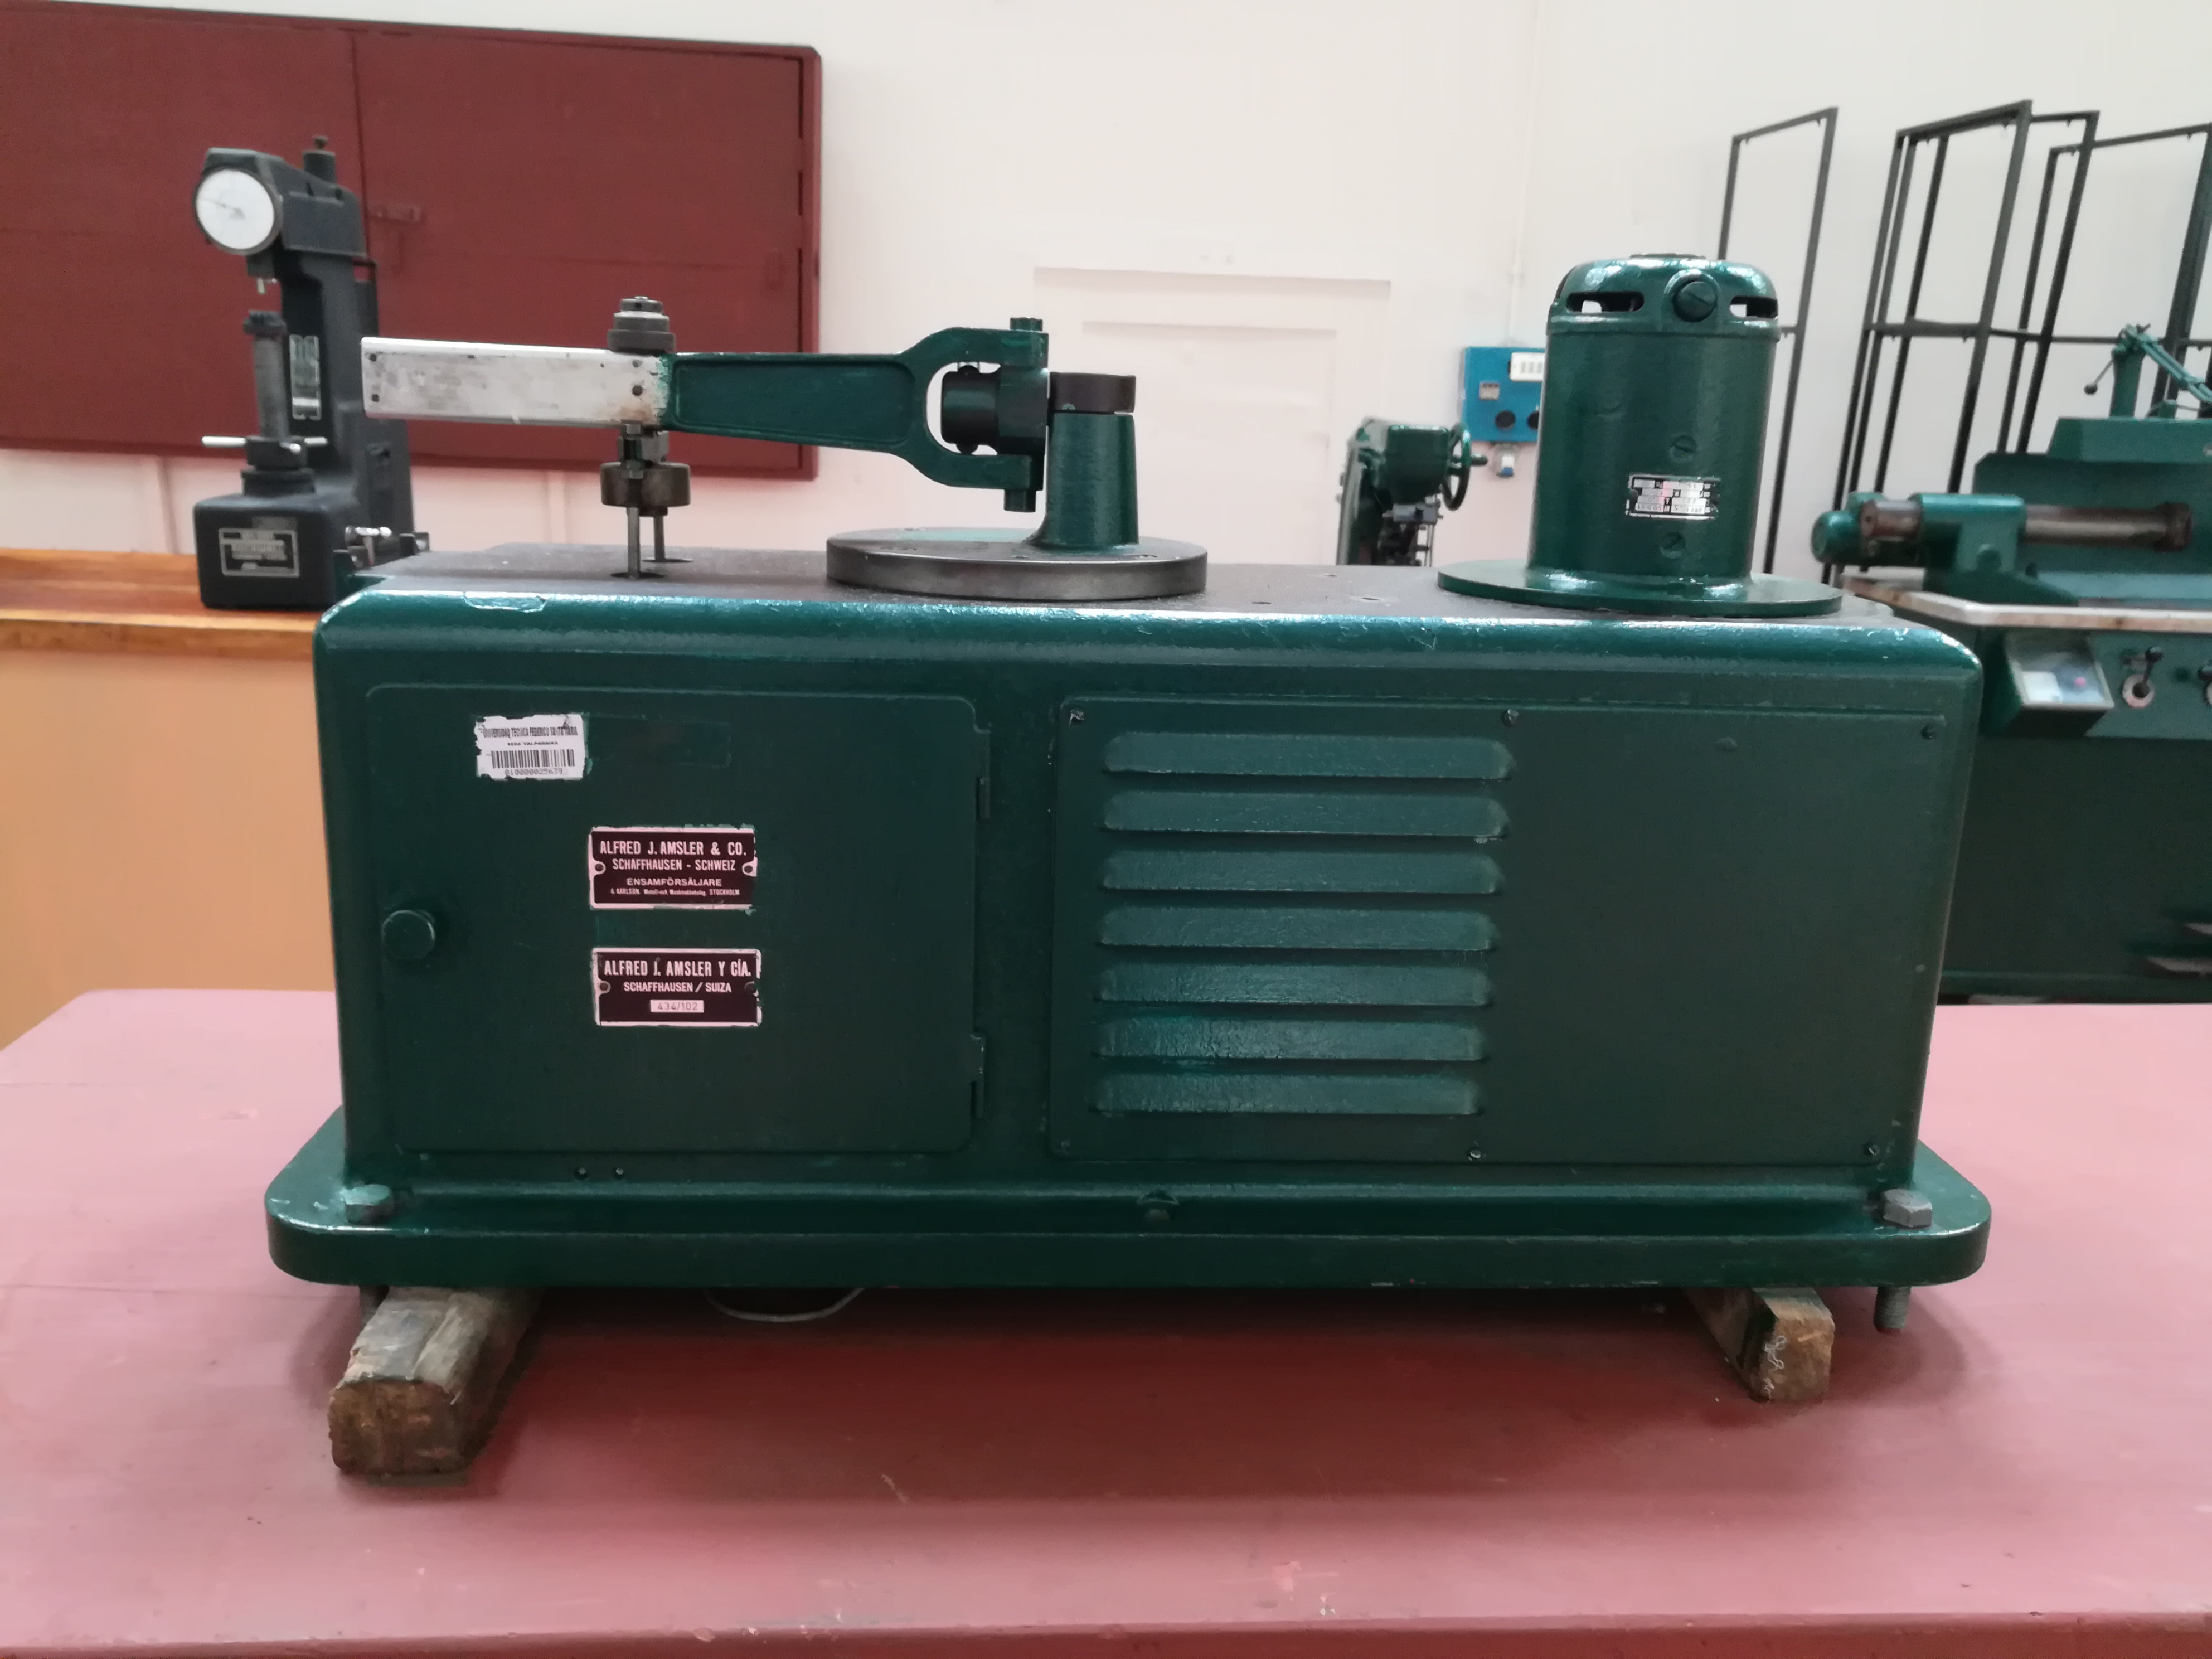
\includegraphics[scale=0.05]{Imagenes/maq_del.jpg}
\label{fig:maq_del}
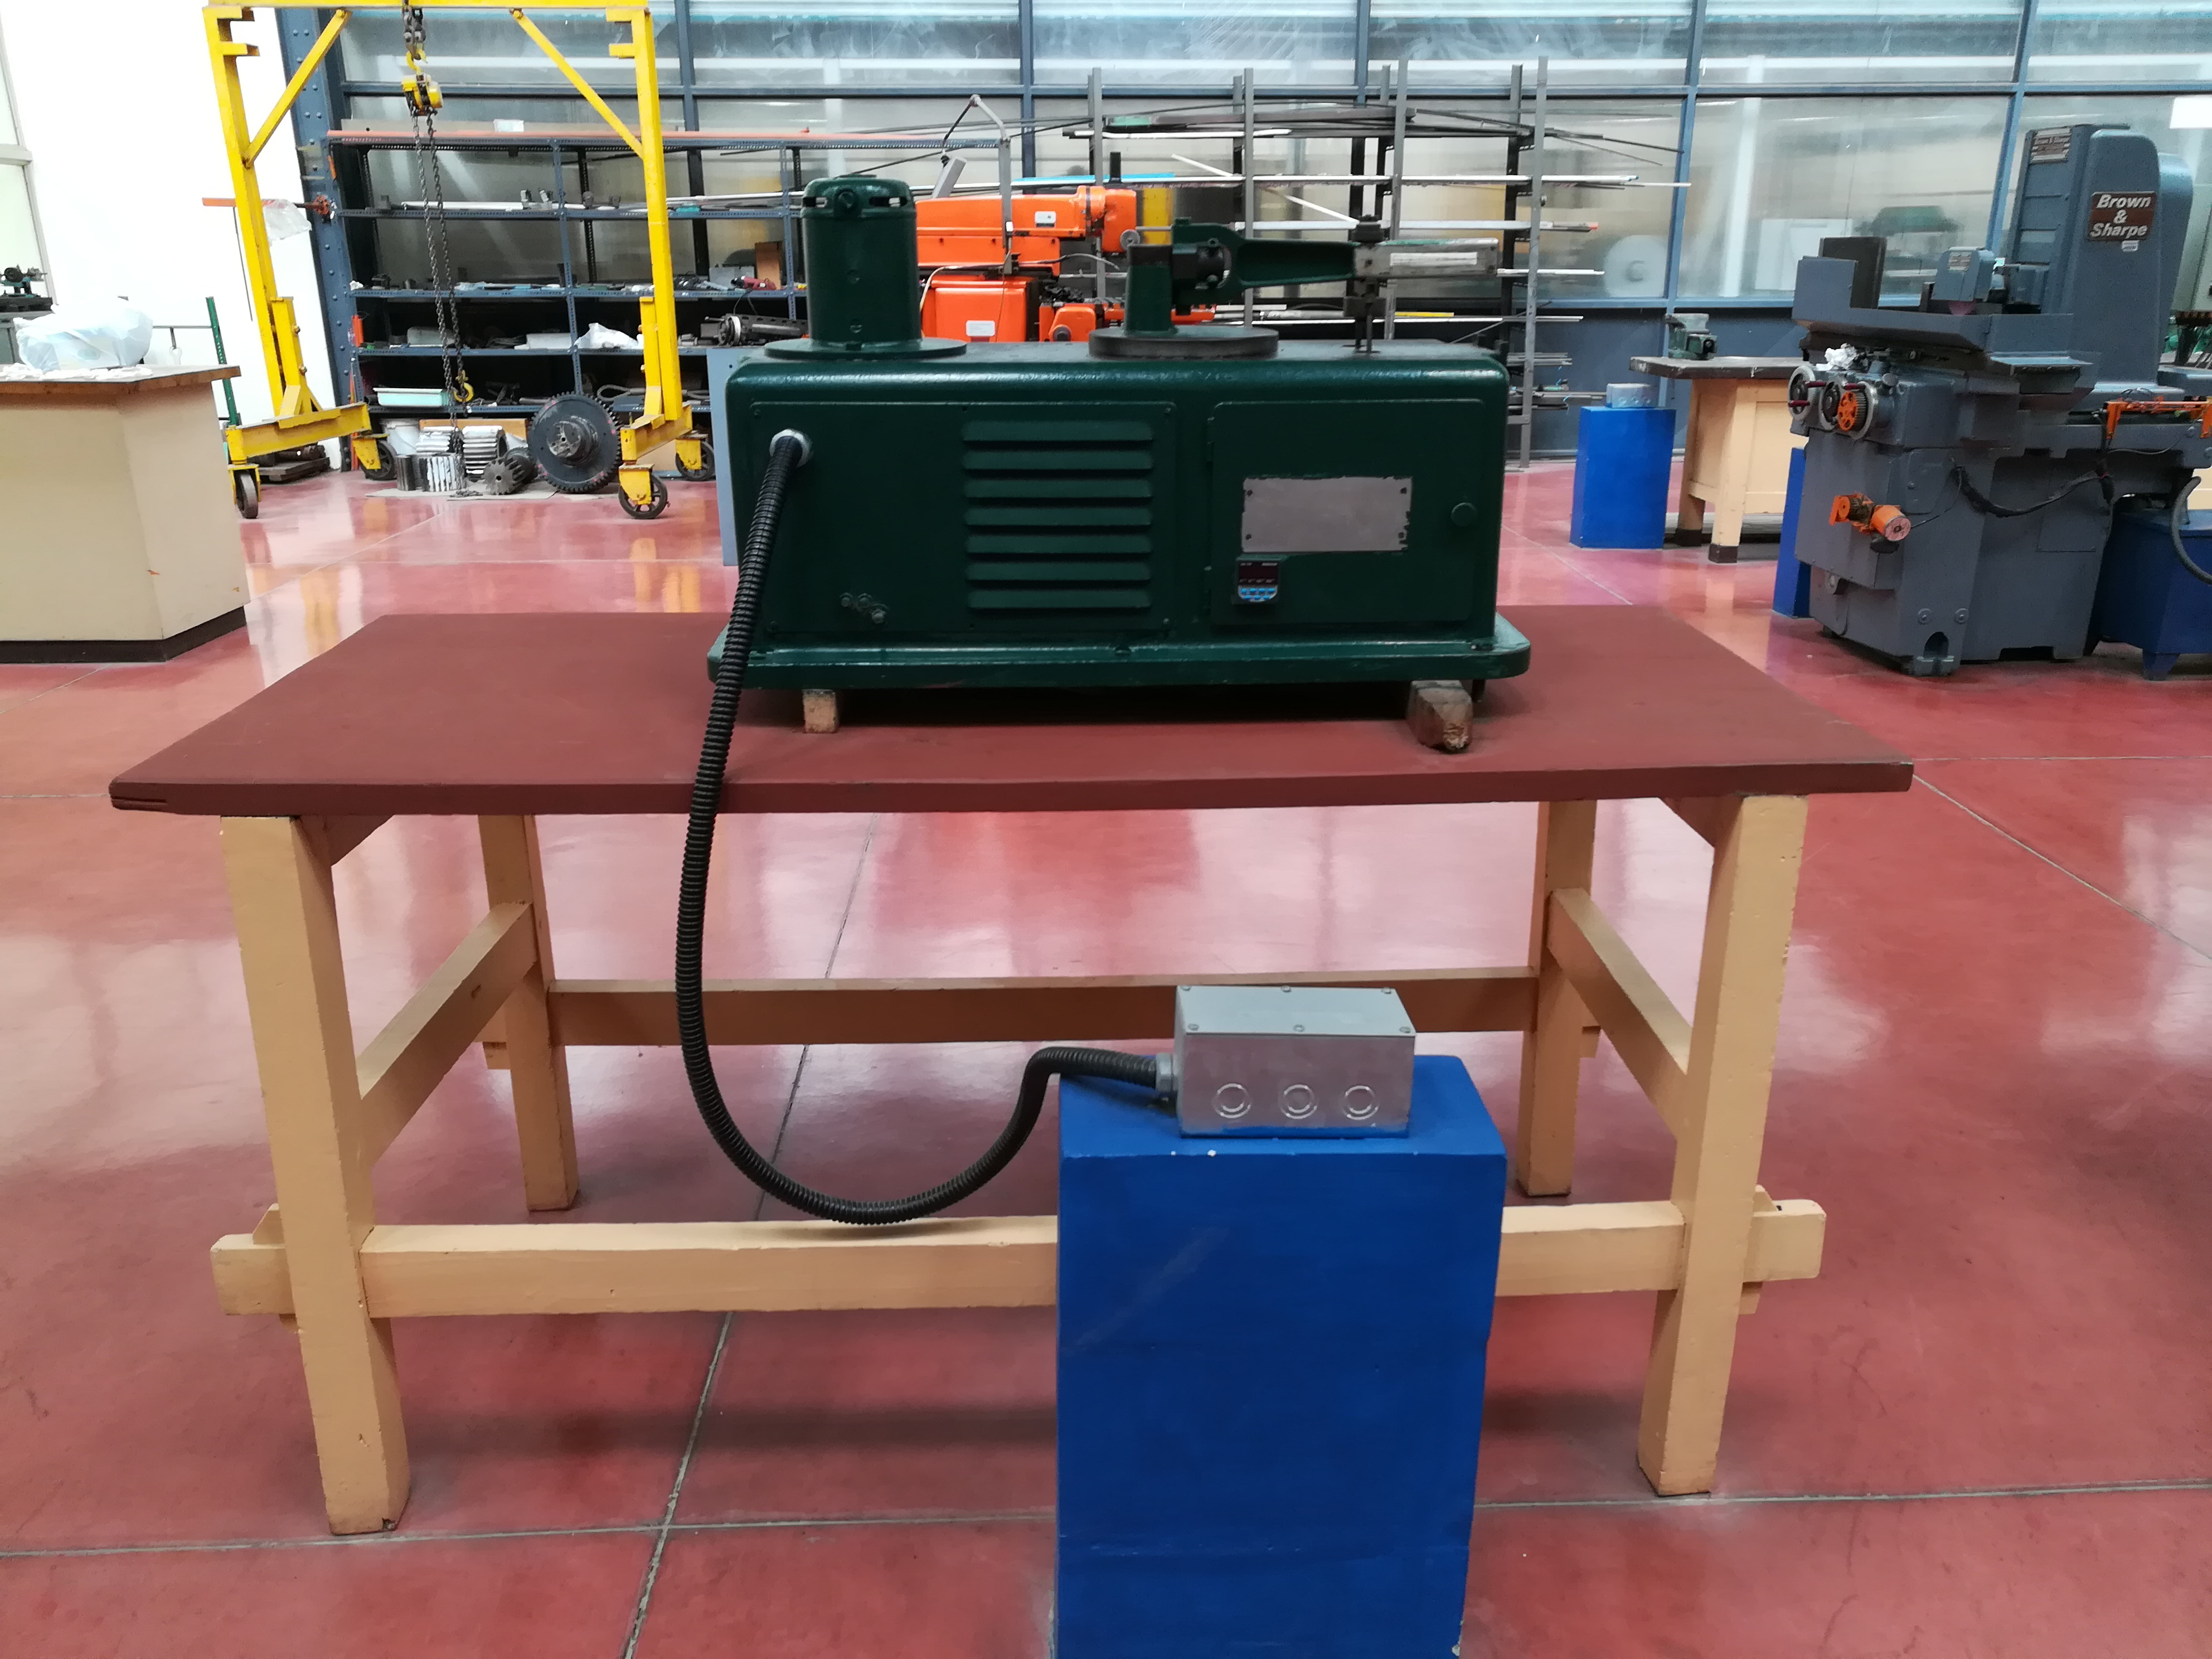
\includegraphics[scale=0.05]{Imagenes/maqfull_post.jpg}
\label{fig:maqfull_post}
\caption{Máquina de fatiga en flexión en el laboratorio de tecnología mecánica}
\label{fig:maq_fat}
\end{figure}

\subsection{Estado actual y antecedentes}
Actualmente la máquina no puede ser utilizada por no estar anclada, estando apoyada sobre dos listones de madera, que a su vez, están sobre una mesa de madera como se aprecia en la figura REF. Por consiguiente, la máquina al ser utilizada comienza a vibrar, saltar y desplazarse lateralmente, lo que impide su uso prolongado por motivos de seguridad. Es decir, no es posible realizar correctamente un ensayo de fatiga de ningún material ni configuración.

A partir de información verbal entregada por el profesor Fernando Rojas, se cree que la máquina fue adquirida por el departamento hace, al menos, 50 años atrás. Fue fabricada en Suiza por \textit{Alfred J. Amsler \& Co.} y su estructura completa es de acero fundido. Previo a la modificación actual del laboratorio, la máquina se encontraba anclada al piso con un bloque de concreto que fue demolido durante la remodelación, momento desde el cual se encuentra sin una solución definitiva. Más aún, varios equipos y máquinas de ensayo del laboratorio no se encuentran ancladas al piso ni con una instalación definitiva impidiendo su uso.

La única modificación que posee la máquina, según la información recopilada, consiste en el cambio del contador de revoluciones o ciclos realizados en un ensayo de fatiga. Esta actualización consistió en sacar el contador mecánico original y reemplazarlo por un contador electrónico, el cual tiene sus controles y el display adosada a su estructura, como se puede apreciar en la figura \textcolor{red}{agregar imagen del contador}. 

El sistema eléctrico de la máquina permanece intacto, la cual se encuentra conectada a la red de la universidad. Conserva su motor eléctrico original junto a un conjunto eléctrico cuya función es suministrar energía de manera continua y estable al motor, para evitar que el ensayo de fatiga se pueda ver afectado por problemas y las variaciones del suministro eléctrico. El motor es de \textcolor{red}{corriente continua} con velocidad constante y sus especificaciones se pueden ver en la tabla \ref{tab:motor_maq}:

\begin{table}[h]
\centering
\begin{tabular}{ll}
\hline
Especificaciones Motor                            & Valor   				\\ \hline
Tensión                                           & 220 {[}V{]}        		\\
Corriente                                         & 0,8 {[}A{]}        		\\
Factor de potencia ($\cos \varphi$)				  & Sin información    		\\
Potencia                                          & 100 {[}W{]}        		\\
Velocidad                                         & 1500 {[}rev/min{]} 		\\ \hline
\end{tabular}
\caption{Especificaciones del motor de la máquina de fatiga.}
\label{tab:motor_maq}
\end{table}

Otro elemento distinto al original consiste en la correa de transmisión entre el motor eléctrico y el disco desbalanceado. La original consistía en una correa de cuero plana y cruzada, sin información respecto a su empalme. La correa actual consiste también en una correa plana y cruzada, sin embargo, su material es tela y el empalme es realizado a mano con hilo acerado. Cabe destacar que lo poco usual de las dimensiones, características y la necesidad de hacer el empalme en la misma máquina, dificulta la búsqueda de una correa que pueda cumplir de manera óptima la transmisión de potencia. Parte de estas dificultades se deben a que el sistema de transmisión no ha sido modificado donde sus poleas tienen dimensiones, tanto de diámetro como de ancho, que no están normalizadas o se encuentran fuera de catálogo de mucho proveedores. 

Por otro lado, los elementos de agarre de la probeta no tienen modificaciones conocidas, tanto el brazo que recibe el movimiento como el agarre empotrado a la estructura de la máquina. La fabricación de las probetas utilizadas se realiza en el mismo laboratorio a partir de acero AISI 1020 o 1040, el cual para conseguir las dimensiones de la figura REF. se debe cortar y tornear.

Finalmente, para realizar los ensayos en distintas configuraciones existen distintas masas (figura REF) que desequilibran el disco rotativo, como se verá en la sección \ref{sec:funcionamiento}, y estas combinaciones se especifican en una tabla de cargas (Anexo REF). Sin embargo, se desconoce el origen, y en consecuencia, la fiabilidad de la información contenida en esta tabla.

\subsection{Funcionamiento}
\label{sec:funcionamiento}
La máquina de fatiga tiene como objetivo lograr que para cada ciclo se ejerza el mismo esfuerzo determinado sobre la probeta, en forma de flexión. Para lograr esto, el mecanismo utilizado es un disco desequilibrado girando a una velocidad constante $\dot{\theta}$, la fuerza es transmitida hasta un brazo que sostiene a su vez a la probeta, generando flexión en la probeta con un doble empotramiento. La velocidad $\dot{\theta}$ del disco se transmitida desde el motor eléctrico a través de poleas y una correa de transmisión en una relación de 1:1 \textcolor{red}{revisar}, a una velocidad de 1500 revoluciones por minuto. Así, para realizar las mediciones de fatiga a distintas cargas se modifica el desequilibrio del disco a través de un conjunto de masas, mostradas en la figura REF, que permiten generar distintas configuraciones y, por consiguiente, esfuerzos en la probeta.

\textcolor{red}{Agregar imagen de contrapesos}

Los elementos utilizados para desbalancear son 6 discos pequeños de X \textcolor{red}{medir radio masas} a Y de diámetro. Estos son enumerados del 1 al 5, donde el 1 es el más liviano y el 5 el más pesado, todos de distinto peso y el quinto se encuentra repetido. Estas se colocan en los extremos del disco giratorio, como se ve en la figura REFimagendisco, dependiendo de la carga que se desee generar. Para conocer que configuración corresponde a cada esfuerzo aplicado sobre la probeta, se utiliza la tabla de cargas explicada a continuación.


Esta tabla, con 3 columnas de información como se ve en el Anexo REF, nos entrega el esfuerzo normal $\sigma$, cortante $\tau$ y la combinación necesaria para generar esos esfuerzos. Los números entre paréntesis nos indican cuantos contrapesos se deben apilar en cada perno adosado al disco giratorio, los cuales llamaremos soportes de contrapeso (SC). Así, la tabla nos señala que la fuerza es función de la diferencia de masa entre cada soporte, es decir, la suma de las masas de cada paréntesis. A modo de ejemplo, en la tabla \ref{tab:ejemplo_config} se han colocado las 4 primeras filas de la tabla de cargas, añadiendo 4 columnas con información sobre el peso de cada combinación. En las columnas $m_1$ y $m_2$ se aprecia la suma de cada masa colocada en sus soportes de contrapeso señalado por la columna de ``Combinación''. Las columnas siguientes representan $\Delta m = m_1-m_2$ y $m_{total}=m_1+_2$. Como se puede apreciar, los esfuerzos normales y cortantes aumentan en la medida que $\Delta m$ de cada combinación aumenta, independiente de $m_{total}$.

\begin{table}[h]
\centering
\label{tab:ejemplo_config}
\begin{tabular}{@{}cclllll@{}}
\toprule
$\sigma \left[\frac{\text{kg}_f}{\text{cm}^2}\right]$ & {$\tau \left[\frac{\text{kg}_f}{\text{cm}^2}\right]$} & Combinación     & $m_1$ {[}g{]} & $m_2$ {[}g{]} & $\Delta m$ {[}g{]} & $m_{total}$ {[}g{]} \\ \midrule
40                                                   & 20                                                                    & (5) - (1+2+3+4) & 30,9199       & 30,5071       & 0,4128             & 61,427              \\
80                                                   & 40                                                                    & (1) - (0)       & 0,7582        & 0             & 0,7582             & 0,7582              \\
120                                                  & 60                                                                    & (5) - (4+2+3)   & 30,9199       & 29,7489       & 1,171              & 60,6688             \\
160                                                  & 80                                                                    & (2) - (1)       & 2,2969        & 0,7582        & 1,5387             & 3,0551              \\ \bottomrule
\end{tabular}
\caption{Tabla de configuración de las masas modificada, mostrando el peso, su diferencia y el total para cada combinación}
\end{table}

Con esto, la probeta a ensayar estará sometida a un esfuerzo en flexión, empotrada en ambos lados por la mordaza del brazo y la mordaza empotrada a la estructura de la máquina, ambas mostradas en la figura REF. Una vez que se haya escogido la configuración de masas y la probeta se encuentre en su posición, una pequeña barra con una manilla ubicada entre las barras de acero, como se aprecia en la figura REF, eleva ambas barras con el objetivo de evitar que oscile durante el encendido y aceleración del motor hasta su velocidad final, dejando a la barra en una configuración de empotrado y apoyo simple. Una vez que el motor alcanza una velocidad estable, el sostén es girado nuevamente para dejar al disco giratorio en posición de empotrado-libre. Este sostén, permite que el ensayo de fatigue se realice siempre a una frecuencia constante y evitar la transición inicial del motor. Una vez que la probeta se fracture, provocarán un aumento en la amplitud de las oscilaciones del disco las cuales activarán el freno automático (figura REF) para detener el motor y, por lo tanto, el ensayo. Gracias a este sistema, es posible conocer la cantidad de ciclos que realizados hasta el momento de fractura sin la necesidad de supervisar de manera continua el ensayo.

\textcolor{red}{Mordazas}
\subsection{Mediciones}
Para realizar un correcto diseño de la estructura soportante y la compresión de su funcionamiento, se hace vital poder contar con información confiable para obtener resultados correctos. Para esto, las mediciones se dividirán según su objetivo en el desarrollo de este trabajo.
\subsubsection{Diseño de estructura}
Las medidas de la mesa actual son: 
\begin{itemize}
	\item Ancho = 74,5 cm
	\item Largo = 177 cm
	\item Altura = 91 cm
\end{itemize}
Por otro lado, para diseñar correctamente la estructura se deben conocer las dimensiones de la máquina, su peso y la ubicación de los pernos de anclaje, así como también el tipo de perno utilizado. La figura REF\textcolor{red}{realizar diagrama con vistas frontal y lateral de la maquina con sus dimensiones} es un esquema representativo de la máquina, mostrando sus dimensiones de ancho, alto y largo, las dimensiones de su base y la ubicación de sus pernos. La masa de toda la máquina se aproximó a partir de las dimensiones externas, estimando el grosor de sus paredes y considerando el peso específico del acero fundido, sobrestimando el valor del espesor de sus paredes como factor de seguridad. Considerando el peso específico del acero $\rho_{acfund} = 7850 \, [Kg/m^3]$, entonces la masa total calculada es:

\[ \left. 
\begin{array}{ll}
V_{base} &= (3,3\cdot 91\cdot 39 - 3\cdot 88\cdot 37)\; \text{cm}^3	\\
V_{superior} &=(30,2\cdot 84\cdot 32 - 26\cdot 78\cdot 28,5) \; \text{cm}^3	\\
\end{array}
\right\} \\
\quad V_{b+s} = 25323,3 \; \text{cm}^3 \]
\begin{equation}
	m_{maq} = \rho_{ac. fundido} \cdot V_{b+s} = 198,8 \: kg \approx 200 \: kg
\end{equation}

\subsubsection{Caracterización de los componentes}
\subparagraph{Sistema de transmisión}
El sistema de transmisión está compuesto por el motor eléctrico, cuyas características se detallaron anteriormente, la correa de transmisión y ambas poleas. Las dimensiones y características de las poleas conductora y conducida, como también de la correa se encuentran en la tabla \ref{tab:sist_transmision}. 

\begin{table}[h]
\centering
\begin{tabular}{@{}ll@{}}
\toprule
Características          & Valor   			\\ \midrule
Diámetro polea motriz    & 48 mm   			\\
Diámetro polea conducida & 47,5 mm 			\\
Relación de poleas		 & $\approx$ 1 (-) 	\\
Ancho correa             & 10 mm   			\\
Longitud correa          & 1235 mm 			\\
Configuración            & Cruzada 			\\ \bottomrule
\end{tabular}
\caption{Datos del sistema de transmisión}
\label{tab:sist_transmision}
\end{table}

\subparagraph{Barras de acero}
El conjunto de barras de acero que sostienen el disco en empotrado-libre, tienen medidas levemente distintas para las superiores respecto a las inferiores, separadas por una distancia de 32 mm. La tabla \ref{tab:medidas_barrasacero} muestra las medidas de cada una.
\begin{table}[h]
\centering
\begin{tabular}{@{}lll@{}}
\toprule
Medida  & Barras superiores {[}mm{]} & Barras inferiores {[}mm{]} \\ \midrule
Espesor      & 5,7                        & 5,8                        \\
Ancho        & 25,1                       & 25,2                       \\
Largo        & 333                        & 333                        \\ \bottomrule
\end{tabular}
\caption{Medidas de las barras de acero según su posición}
\label{tab:medidas_barrasacero}
\end{table}

\subparagraph{Sistema de transmisión de fuerzas}
El brazo principal (figura REF) que ejerce la fuerza sobre la probeta proveniente del disco desbalanceado, está constituido por tres partes principales. La primera de ellas es la parte trasera, con forma regular de paralelepípedo, está hecho de una aleación de aluminio y dos tercios de su longitud es ahuecada. La segunda y principal, está hecha de acero fundido y añade el mayor porcentaje de masa al total del brazo. Finalmente, la última parte consiste en la mordaza, unida a la sección principal con dos pernos que permiten ajustar su posición. La longitud total del brazo es de 359 mm y su masa total 2,305 kg.

\textcolor{red}{Imagen brazo-mordaza}

La transmisión de la carga entre el disco desbalanceado y el brazo se da a través de dos barras de acero, uno a cada lado del disco, de diámetro 6,2 mm y largo de 169 mm.

\subparagraph{Disco desbalanceado}
En base a las características visuales y auditivas del disco, se cree que está construido en alguna aleación de aluminio. Su radio $R_d =$ 112 mm y espesor de . 

La masa de cada contrapeso, medidos en el laboratorio de metalúrgica con pesas blablabla.
\begin{table}[H]
\centering
\begin{tabular}{@{}cc@{}}
\toprule
Contrapeso & Masa {[}g{]} \\ \midrule
1          & 0,7582       \\
2          & 2,2969       \\
3          & 6,8541       \\
4          & 20,5979      \\
5          & 30,9199      \\ \bottomrule
\end{tabular}
\caption{Masa de cada contrapeso utilizado}
\label{tab:masa_contrapesos}
\end{table}


\section{Diseño de estructura}
El proceso de diseñar la estructura hasta su resultado final pasó por distintas etapas. Esto por el proceso de aprendizaje y comprensión de la norma de calculo de madera NCh 1198, como también por la restricción y disponibilidad de materiales, tecnología o medidas acorde a las necesidades. El diseño presentado en este trabajo se muestra en la figura REF, hecho principalmente de madera, junto a elementos de acero. El objetivo de esta estructura es fijar y soportar la máquina de fatiga tanto en reposo como en operación, buscando como características su durabilidad, lo modular de las piezas y la opción de modificarla en el futuro.

\textcolor{red}{imagen de vista en perspectiva}

La metodología de su diseño, se separará en las distintas etapas que se realizó y los requerimientos que surgieron a partir de estas. Finalmente, se realizó una simulación estática y modal para comparar los cálculos realizados y conocer su frecuencia natural, respectivamente.
\subsection{Diseño en acero}
La estructura se diseño para que la conexión con la máquina de fatiga fuera a través de pletinas de acero, utilizando los pernos existentes. Las pletinas, a su vez , están conectadas mediante pernos a las vigas principales de madera de cada extremo. Para llevar acabo los cálculo, se hará como suposición que cada pletina esta con un empotramiento en cada extremo, con dos cargas distribuidas. La primera de ellas es el apoyo de la maquina sobre la pletina y, la segunda, el peso propio del acero. Por lo tanto, la figura REF muestra el diagrama de las cargas que actúan y las distancias a utilizar. 

\textcolor{red}{Diagrama de cargas}

Por otro lado, al no conocerse la distribución de masa de la maquina de fatiga, se considerará la carga distribuida en cada pletina como:
\begin{equation}
	 q_{maq} = \frac{0,75\cdot m_{maq}}{c} = 384,62 \; [\text{kg/m}]
\end{equation}
Donde $m_{maq}$ es la masa estimada en \ref{eq:masa_maquina}, multiplicada por 0,75 como factor de seguridad por la distribución irregular de peso de la máquina. Para obtener el esfuerzo máximo flector es necesario conocer la geometría de la viga, motivo por la cual se iteró entre las distintas opciones disponibles en el mercado de pletinas o barras planas de acero. Por razones estipuladas en la norma NCh 1198, la conexión entre la pletina de acero y la viga principal de madera se debe realizar con un mínimo de dos pernos, por lo tanto, se escogió el ancho máximo del mercad. Así, la tabla \ref{tab:dimycar_pletina} muestra las dimensiones de la pletina escogida.
\begin{table}[h]
\centering
\begin{tabular}{@{}ll@{}}
\toprule
Características pletina			       			& Valor        \\ \midrule
Espesor ($h_p$) {[}mm{]}              			& 8            \\
Ancho ($b_p$) {[}mm{]}               		    & 100          \\
Material    		                		    & A270ES	   \\
Carga distribuida ($q_{ac}$) {[}kg/m{]}		    & 6,28         \\ \bottomrule
\end{tabular}
\caption{Dimensiones y características de la viga de acero}
\label{tab:dimycar_pletina}
\end{table}

Por ende, el cálculo de la reacción en sus apoyos, el momento y esfuerzo flector máximo queda expresado por las ecuaciones \ref{eq:reaccion_acero}, \ref{eq:mtofleca_acero} y \ref{eq:esfmax_acero}, respectivamente. Estas fueron calculadas respecto al punto $A$ (o $B$, por simetría), donde se encuentra el momento flector máximo.

\begin{subequations}
	\begin{gather}
		R_A = g\left(\frac{m_{maq}}{2} + \frac{q_{ac}L}{2}\right) \label{eq:reaccion_acero}\\ 
		M_A = \left(\frac{gcq_{maq}}{24L}\right) \left(3L^2 - 4c^2 + \frac{6bc^2}{L} - \frac{3c^3}{L}\right) + \left(\frac{gq_{ac}L^2}{12}\right) \label{eq:mtofleca_acero} \\
		\sigma_{max} = \frac{M_A \cdot h_p}{2I} \label{eq:esfmax_acero}
	\end{gather}
\end{subequations}

Así, los valores obtenidos son:
\begin{itemize}
	\item $R_A = 754,85$ [N]
	\item $M_A = 100,97$ [Nm]
	\item $I = 4266,6$ [mm$^4$]
	\item $\sigma_{max} = 94,66$ [MPa]
\end{itemize}

\textcolor{red}{agregar fatiga}

\subsection{Diseño en madera}
La elección de la madera como elemento principal de construcción se debió por su capacidad de disipar las vibraciones y la relación entre su resistencia y el peso, volviendo la estructura más liviana y útil para las necesidades. Para realizar los cálculos de la madera y sus uniones, se utilizó la norma \textbf{NCh 1198 Of. 91 -- Madera: Construcciones en madera -- Cálculo}, mostrada en el anexo \ref{ch:anexo_a}. Las dimensiones del diseño de la estructura se realizaron considerando dejar el espacio necesario para la operación de la máquina, conservando la altura actual de 900 [mm]. Si bien en el presente trabajo se expondrán los cálculos de una especia maderera y sus respectivas dimensiones, se realizaron cálculos con otras especies y en otros formatos para añadir flexibilidad al diseño propuesto. Las maderas consideradas en el trabajo son el pino Oregón, pino Radiata y la línea de pino radiata encolado Hilam de Arauco. Los resultados mostrados en la sección siguiente son los obtenidos al escoger el pino Oregón en formato de 110x110 [mm]. Los valores de las tensiones admisibles para distintas especies madereras se obtienen de la tabla 4 de la sección 6.2 de la NCh 1198, sin embargo, para la madera laminada encolada se encuentran en la norma NCh 2165. Finalmente, para la sección de diseño en madera se utilizará la nomenclatura utilizada por la norma NCh 1198, para evitar confusiones al momento de consultar el anexo o la norma misma.

\textcolor{red}{añadir tabla con las dimensiones de la madera}

\subsection{Cálculo de cargas en estructura de madera}
Para identificar las distintas partes de madera en la estructura, se utilizará la figura REF como referencia. Tanto las vigas A, C, D y el pilar B, están diseñados de la misma madera y formato. En el anexo REF se pueden apreciar los planos del diseño de la estructura propuesta y sus uniones.

\textcolor{red}{añadir imagen de vigas A, B, C y D}

Como se nombró anteriormente, la madera utilizada será pino oregón, el cual bajo las consideraciones de la tabla \ref{tab:tabla3_1198} se considerará como seca tanto en construcción como en servicio al estar en un ambiente cerrado sin calefacción, como se señala en la sección \ref{sec:contenido_humedad} de contenido de humedad. Los valores de densidad, tanto anhidra como normal, se pueden obtener del Anexo E de la norma, a partir de este, la tabla \ref{tab:densidad_oregon} muestra los valores del pino oregón.

\begin{table}[h]
\centering
\resizebox{\textwidth}{!}{%
\begin{tabular}{@{}ccccc@{}}
\toprule
\multirow{2}{*}{\begin{tabular}[c]{@{}c@{}}Especie \\ maderera\end{tabular}} & \multicolumn{2}{c}{Densidad anhidra (kg/m$^3$)}                                                                                                & \multicolumn{2}{c}{Densidad normal (kg/m$^3$)}                                                                                                     \\ \cmidrule(l){2-5} 
                                                                             & \begin{tabular}[c]{@{}c@{}}Valor medio \\ $\rho_o$\end{tabular} & \begin{tabular}[c]{@{}c@{}}Valor característico\\ $\rho_{o,k}\,^{\dagger}$\end{tabular} & \begin{tabular}[c]{@{}c@{}}Vallor medio \\ $\rho_{12}$\end{tabular} & \begin{tabular}[c]{@{}c@{}}Valor caracerístico\\ $\rho_{12,k}\,^{\dagger}$\end{tabular} \\ \midrule
Pino oregón                                                                  & 410                                                             & 326                                                                          & 441                                                                 & 350                                                                          \\ \bottomrule
\end{tabular}%
}
\caption{Valores de la densidad normal y anhidra del pino oregón. $^{\dagger}$: Definido con el percentil 5\% de exclusión.}
\label{tab:densidad_oregon}
\end{table}

\subparagraph{Tensiones admisibles y módulo de elasticidad del pino oregón.}
Para la determinación de estos valores es necesario catalogar el grado de calidad, si corresponde a madera verde o seca y la clasificación de la madera del pino oregón. El agrupamiento de las maderas crecidas en Chile se encuentran en el anexo A de la norma NCh 1198, según la cual el pino oregón se clasifica en el grupo ES 5 para madera seca y se asumirá un grado estructural N$^{\circ}$ 4. Con esta información, a través de la tabla 6 de la norma, obtenemos que la clase estructural es F8. Con esto, la tabla 4 y 5 entrega la información de las tensiones admisibles y el módulo de elasticidad. Así, la tabla REF los valores del pino oregón utilizado en este trabajo.

\begin{table}[h]
\centering
\resizebox{\textwidth}{!}{%
\begin{tabular}{@{}ccccccc@{}}
\toprule
\begin{tabular}[c]{@{}c@{}}Clase\\ Estructural\end{tabular} & \begin{tabular}[c]{@{}c@{}}Flexión\\ $F_f$\end{tabular} & \begin{tabular}[c]{@{}c@{}}Compresión\\ Paralela $F_{cp}$\end{tabular} & \begin{tabular}[c]{@{}c@{}}Compresión\\ Normal $F_{cn}$\end{tabular} & \begin{tabular}[c]{@{}c@{}}Tracción \\ Paralela $F_{tp}$\end{tabular} & \begin{tabular}[c]{@{}c@{}}Cizalle\\ $F_{cz}$\end{tabular} & \begin{tabular}[c]{@{}c@{}}Módulo de\\ elasticidad en\\ flexión $E_f$\end{tabular} \\ \midrule
F8                                                          & 8,6 (MPa)                                               & 6,6 (MPa)                                                              & 4,1 (MPa)                                                            & 5,2 (MPa)                                                             & 0,86 (MPa)                                                 & 6,9 (GPa)                                                                          \\ \bottomrule
\end{tabular}%
}
\caption{Tensiones admisibles y módulo de elasticidad en flexión para madera de pino oregón según su clase estructural.}
\label{tab:tadm_oregon}
\end{table}

\subparagraph{Factores de modificación.}
Dada las condiciones en las que trabajará la madera, se deben calcular tres factores de modificación que afectan de manera global a la madera, sin embargo el factor de modificación por trabajo conjunto, $K_C$, no se considera en este caso. La modificación por contenido de humedad se calcula con un factor $\Delta R$ y por la diferencia entre la humedad de la madera y una humedad del 12\%, $\Delta H$. Considerando una humedad de la madera del 15\%, entonces los valores de $K_H$ para cada solicitación son los siguintes se muestran en la tabla \ref{tab:kh_oregon}.
\begin{table}[h]
\centering
\resizebox{\textwidth}{!}{%
\begin{tabular}{ccccccc}
\hline
\begin{tabular}[c]{@{}c@{}}Factor de \\ modificación\\ por humedad\end{tabular} & \begin{tabular}[c]{@{}c@{}}Flexión\\ $F_f$\end{tabular} & \begin{tabular}[c]{@{}c@{}}Compresión\\ Paralela $F_{cp}$\end{tabular} & \begin{tabular}[c]{@{}c@{}}Compresión\\ Normal $F_{cn}$\end{tabular} & \begin{tabular}[c]{@{}c@{}}Tracción \\ Paralela $F_{tp}$\end{tabular} & \begin{tabular}[c]{@{}c@{}}Cizalle\\ $F_{cz}$\end{tabular} & \begin{tabular}[c]{@{}c@{}}Módulo de\\ elasticidad en\\ flexión $E_f$\end{tabular} \\ \hline
$K_H$                                                                           & 0,999385                                                & 0,999385                                                               & 0,999385                                                             & 0,99952                                                               & 0,999199                                                   & 0,999556                                                                           \\ \hline
\end{tabular}%
}
\caption{Valores del factor de modificación para el pino oregón.}
\label{tab:kh_oregon}
\end{table}

Por otro lado, el factor de modificación por duración, $K_D$, se aplica a través de la ecuación \ref{eq:k_d}, donde la duración de la carga $t$ se aplica en segundos. También, la norma incluye el gráfico de $K_D$ siendo una opción para su cálculo. Los valores admisibles que se señalan en la norma corresponden a una vida útil de 10 años de duración, sin embargo, para una vida útil indefinida el valor de $K_D$ corresponde a 0,9. Este factor de modificación no afecta al módulo de elasticidad ni a la tensión admisible de compresión normal.
\begin{equation} \label{eq:k_d}
	K_D = \frac{1,747}{t^{0,0464}} + 0,295
\end{equation}

\subsubsection{Viga principal, A}
Es la viga que soporta la carga de las pletinas que sostienen a la máquina y a su vez descansa la carga en los pilares B. Para realizar los cálculos de esfuerzo se consideró un doble empotramiento en cada extremo, con tres cargas distribuidas que representan la carga de las pletinas de acero, $q_{pl}$, las cuales se determinarán según la ecuación \ref{eq:q_pl}, y el peso propio de la madera.
\begin{equation}\label{eq:q_pl}
	q_{pl} = \frac{q_{maq}\,c + q_{ac}\,L}{2b_p}
\end{equation}
El diagrama y la distribución de la carga se puede apreciar en la figura REF. Por otro lado, el esfuerzo máximo se presenta en los extremos de la viga. Las ecuaciones \ref{eq:reac_vigappal} y \ref{eq:mto_vigappal}, muestran la obtención de las reacciones y del momento flector máximo.
\begin{subequations}
\begin{gather}
	R_0 = g \left( q_{pl}\cdot b_p + \frac{L\cdot q_{mad}}{2}\right) \label{eq:reac_vigappal}\\
	M_0 = \left(\frac{q_{pl}\cdot g\cdot b_p}{L^2}\right) \left(l_2 l_6^2 + l_6 l_2^2 - \frac{b_p^2}{12}\left( l_6 + l_2\right) \right) + \frac{R_0\cdot L}{6} \label{eq:mto_vigappal} 
\end{gather}
\end{subequations}
Donde los valores obtenidos son:
\begin{itemize}
	\item $R_0 = Q = 795$ [N]
	\item $M_0 = M_{max} = 122,26$ [Nm]
\end{itemize}
Así, la tensión de trabajo $f_f$ se calcula según la ecuación \ref{eq:f_f}, obteniendose el valor:
\begin{equation}
	f_f = 0,551 \quad \text{(MPa)}
\end{equation}
De este modo, la tensión de diseño en la zona flexo-traccionada y flexo-comprimida que se calcula a partir de \ref{eq:ft_dis} y \ref{eq:fv_dis}, respectivamente. Para la zona flexo-traccionada se debe calcular el factor de modificación por altura y para la flexo-traccionada el factor de modificación por volcamiento. El primero se obtiene con la ecuación \ref{eq:khf}, obteniendose el valor de $K_{hf} = 0,916$. Para el factor de volcamiento, se deben verificar el caso que corresponde como se señala en el anexo \ref{ch:anexo_a}, el cual da un valor de $K_v=1$. Por lo tanto, el valor de $F_{ft,dis}$ y $F_{fv,dis}$ son:
\begin{subequations}
\begin{gather}
	F_{ft,dis} = 7,08 \quad \text{(MPa)}\\
	F_{fv,dis} = 7,74 \quad \text{(MPa)} 
\end{gather}
\end{subequations}
Por otro lado, la tensión de trabajo en cizalle se obtiene a partir de la ecuación \ref{eq:f_cz} y la de diseño en cizalle por \ref{eq:cz_dis}. Dado que $K_r=1$ al no haber rebajo de la viga, entonces el valor obtenido para ambas tensiones son:
\begin{gather}
	f_{cz} = 0,098 \quad \text{(MPa)}\\
	F_{cz,dis} = 0,774 \quad \text{(MPa)}
\end{gather}
Finalmente, los valores de factor de seguridad (FS) para cada uno de las tensiones calculadas son los siguientes:
\begin{subequations}
\begin{gather}
	FS_{ft} = 12,85\\
	FS_{fv} = 14,03\\
	FS_{cz} = 7,85
\end{gather}
\end{subequations}

\subsubsection{Pilar de apoyo, B}
El pilar B representa los cuatro apoyos de la estructura, recibiendo la carga de la máquina y su operación desde la viga principal y transmitiendola hasta el piso. Por la disposición del cuartón, estará sometido a compresión paralela (\ref{sec:cp}). Al igual que en la viga principal, se debe calcular la tensión de trabajo ($f_{cp}$) y la tensión de diseño en compresión paralela ($F_{cp,dis}$). Al ser el mismo formato y especie maderera de la viga principal, su área transversal sigue siendo de 110x110 mm, mientras que el largo del pilar ($L_v$) corresponde a 790 mm.

Para el primero, se obtiene a través de la ecuación \ref{eq:f_cp}, donde la carga $N$ será igual a la reacción obtenida en \ref{eq:reac_vigappal}. Así, su valor es:

\textcolor{red}{Corregir con área modificada por pernos}
\begin{equation}
	f_{cp} = 0,0657 \quad \text{(MPa)} 
\end{equation}
Para el segundo, el cálculo de la tensión de diseño dependerá de la inestabilidad lateral dado por la esbeltez $\lambda$. La longitud efectiva de pandeo se obtiene a través de la tabla 18 de la norma, de la cual se escogerá la configuración de apoyo con impedimento de giros y desplazamiento por un extremo y, para el otro lado, impedimento de giro con libertad de desplazamiento, es decir, $l_p/L_v = 1,5$. De esta forma, los valores obtenidos son:
\begin{gather*}
	l_p = 1,5\cdot L_v = 1,185 \: \text{(m)}\\
	i = \sqrt{\frac{I}{A}} = \sqrt{\frac{0,11^4}{12\cdot 0,11^2}} = 0,032 \: \text{(m)}\\
	\lambda = \frac{l_p}{i} = 37,32 \: \text{(-)}
\end{gather*}
Como $\lambda > 5$, entonces la tensión de trabajo de compresión paralela se debe calcular según \ref{eq:cp_dislambda} y se debe evaluar el factor de modificación por esbeltez $K_{\lambda}$ a partir de \ref{eq:k_lambda}. El coeficiente de proporcionalidad para una madera de grado n$^{\circ}$ 4 es $c = 0,8$ y el módulo de elástico de diseño es $E_{dis} = 6206,2\: \text{(MPa)}$. Por otro lado, la tensión de diseño $F_{cp,dis}$ se obtiene según \ref{eq:cp_dis} y los factores de modificación $K_D$ y $K_H$.
\begin{equation}
	F_{cp,dis} = 5,936 \: \text{(MPa)}
\end{equation}
Con esto, los valores de las constantes y el factor de modificación serán $A = 2,852\;$ (-), $B = 3,754\;$ (-) y $K_{\lambda} = 0,759\:$ (-). Así, el factor de modificación final $F_{cp,\lambda, dis}$ será:
\begin{equation}
	F_{cp,\lambda, dis} = 4,506 \: \text{(MPa)}
\end{equation}
Finalmente, el factor de seguridad con esta configuración es:
\begin{equation}
	FS_{cp,\lambda} = 68,6\: \text{(-)}
\end{equation}

\subsubsection{Viga transversal, C}
Para esta viga se realizará el mismo procedimiento que para la viga A, sin embargo, las solicitaciones son menores y la única carga a la que está sometida es la de su propio peso. Las dimensiones nominales de la tabla son 1x8'' cepillada, es decir, según las tablas de valores \ref{tab:anchodim} y \ref{tab:espdim} son de 19x185 mm y su largo es de 800 milímetro. La carga distribuida de su peso es de $q_{tabla}=1,5$ [kg/m].

Debido a lo bajo de las solicitudes, las tensiones de trabajo en flexión son:
\begin{equation}
	f_f = 3,804 \: \text{(kPa)} 
\end{equation}
Por otro lado, por las dimensiones de la madera usada, el factor de modificación por altura y volcamiento son los siguientes:
\begin{gather*}
	K_{hf} = 0,864\: \text{(-)}\\
	K_{v} = 0,586\: \text{(-)}
\end{gather*}
El cálculo de $K_v$ se realiza con la ecuación \ref{eq:k_v}, porque la esbeltez del límite elástico es menor a la esbeltez de volcamiento.
\begin{gather*}
	\lambda_v = 23,38 \: \text{(-)}\\
	\lambda_{vo} = 21,95 \: \text{(-)}
\end{gather*}
Así, la tensión de diseño en flexión de esta viga es de:
\begin{equation}
	F_f = 3,9235 \: \text{(MPa)}
\end{equation}
\subsection{Uniones}
Las uniones en madera se deben diseñar siguiendo las indicaciones establecidas en la sección 10 de la norma NCh1198, uniones en la madera estructural. Esta considera la condición de la madera en operación, el tipo de unión, la dirección de la solicitación repecto a la dirección de la fibra, el número de elementos de unión, el distanciamiento entre los elementos de unión y el tipo de cizalle. Para el diseño de la estructura se utilizaron tres elementos de unión distintos: tirafondos, pernos \textcolor{red}{ y, en menor medida, clavos.}

\subsubsection{Acero - madera}
Para la unión entre la pletina de acero y la viga principal de madera, se utilizaron dos pernos de grado 2 de 4 \nicefrac{1}{2}'' de largo y  $3/8''$ de diámetro. Como se explica en la sección \ref{sec:union_perno} el mínimo de pernos por unión debe ser dos, con la excepción de que el único perno no esté solicitado en un porcentaje superior al 50\% de su capacidad de diseño. La unión está compuesta por la pletina de acero, seguido por la viga de madera con la dirección de sus fibras normal a las solicitaciones y nuevamente una placa de acero. Finalmente, para el cálculo de la capacidad de carga admisible y tensión admisible de aplastamiento nominal, se recurrirá a las ecuaciones \ref{eq:padm_ad} y \ref{eq:f_ap}, respectivamente. 

Para calcular la capacidad de carga admisible, $P_{ad}$, se utilizaron las indicaciones para cizalle simple, las cuales indican que se determina como el menor valor de la mitad de la carga admisible de cizalle doble entre una pieza central de espesor igual a la pieza más grande y una pieza central igual al dobleasí  del espesor de la pieza más delgada. Para este diseño el valor menor consiste en considerar el espesor central ficticio $e*$ como dos veces el espesor menor, es decir, el espesor lateral $e_l$, así el valor de esbeltez del perno es:  
\begin{equation*}
	\lambda_u = \frac{2\cdot e*}{D} = \frac{2\cdot 8\, \text{mm}}{9,525\, \text{mm}} = 1,679\: \text{(-)}
\end{equation*}
Para obtener los valores de $F_{ap}$ el valor del factor de reducción de zona elástica se obtiene a partir de la densidad anhidra de la madera (tabla \ref{tab:densidad_oregon}, siendo $\eta =$ 2,2. Por otro lado el ángulo $\theta$ es de $\pi/2$ al estar las fuerzas en dirección normal a la fibra de madera. Con esto, se obtiene:
\begin{gather}
	F_{ap} = 3,402 \: \text{(MPa)} \\
	P_{ad,simple} =\frac{P_{ad,doble}}{2} = 259,24 \: \text{(MPa)}
\end{gather}
Para terminar, se debe corroborar que se cumple la desigualdad de la ecuación \ref{eq:padm_ad}, así:
\begin{equation*}
	Z\cdot D^2 = 2131,94 \: \text{(MPa)} \geq 259,24 \: \text{(MPa)}
\end{equation*}

\subparagraph{Espaciamiento}
El espaciamiento entre los pernos se especifica en la sección \ref{sec:espaciamiento_pernos}, de las cuales se obtiene la distancia entre pernos y los bordes es:
\begin{align*}
	S_{bcn} &= 1,5 \, \text{mm} \\
	S_{bdn} &= 0,75 \, \text{mm} \\
	S_p &= 2,625 \, \text{mm}
\end{align*}


\subsubsection{Madera - Madera}
Existen distintos componentes de unión para la conexión de elementos de madera. En este trabajo se utilizó el tirafondo, perno y clavo como elementos principales de unión.  Cada uno de ellos tiene distintas características que los vuelven ventajosos en ciertas situaciones. La utilización del tirafondo se utiliza para unir la viga C con el pilar B y la viga A, por su capacidad de ``empujar'' una madera contra la otra de manera eficiente. Los pernos, por otro lado, se utilizaran para la unión de herrajes entre la viga D y el pilar B, como también en los herrajes de anclaje del pilar B con el piso. En el caso de los clavos, estos se ocupan en los  herrajes o ángulos de apoyo entre las vigas A y B, para evitar su movimiento transversal. Para estos dos últimos elementos de unión, su elección está supeditada a las recomendaciones del fabricante de los herrajes o ángulos, quienes incluyen los valores de carga en la elección de los elementos de unión. Por lo mismo, la caracterización de estos elementos se realizará en la sección de herrajes.

\subsubsection{Tirafondos}
Las indicaciones para el cálculo, espaciamiento e instalación de los tirafondos se encuentran en la sección \ref{sec:tirafondos}. Al igual que el proceso de selección de vigas de madera, se iteró con distintas dimensiones de largo y diámetro. Así el tirafondo escogido fue de $1/4$x3\nicefrac{1}{2}'', lo cual se traduce a partir del anexo M de la norma en las medidas expuestas en la tabla \ref{tab:tirafondo}.
\begin{table}[h]
\centering
\resizebox{\textwidth}{!}{%
\begin{tabular}{@{}cccccl@{}}
\toprule
\begin{tabular}[c]{@{}c@{}}Nomenclatura\\ tirafondo\end{tabular} & \begin{tabular}[c]{@{}c@{}}Diámetro Nominal \\ ($D_v$ o $D$) [mm]\end{tabular} & \begin{tabular}[c]{@{}c@{}}Diámetro de rosca\\  ($D_R$) [mm]\end{tabular} & \begin{tabular}[c]{@{}c@{}}Largo roscado\\  (R) [mm]\end{tabular} & \begin{tabular}[c]{@{}c@{}}Largo vástago\\ (V) [mm]\end{tabular} & \begin{tabular}[c]{@{}l@{}}Largo punta\\ (P) [mm]\end{tabular} \\ \midrule
$1/4$x3\nicefrac{1}{2}''                                         & 6,4                                                                            & 4,4                                                                       & 51                                                                & 38                                                               & 4,8                                                            \\ \bottomrule
\end{tabular}%
}
\caption{Dimensiones del tirafondo utilizado}
\label{tab:tirafondo}
\end{table}

Para su instalación, la norma indica que es necesario realizar perforaciones guías, las cuales están en función de sus características. Así el agujero tendrá dimensiones para la zona del vástago y otra para la zona con rosca. Para la zona del vástago, el agujero deberá tener las dimensiones del diámetro nominal $D_v$ y el largo V. Para la segunda zona, la madera de pino oregón se categoriza en el grupo B según su densidad anhidra, a partir de la tabla 38 de la norma. Con esta información el largo del agujero debe ser de R - P  y el diámetro del entre el 60\% y el 70\%.
\subparagraph{Solicitaciones de extracción lateral}
La carga admisible de extracción lateral se calcula según la ecuación \ref{eq:pel_ad}. El valor K se obtiene a partir de la tabla 39 de la norma a partir de si la madera utilizada es conífera o latifoliada y su densidad anhidra. El pino oregón es una madera conífera y, según su densidad, el valor de K es de 11,7. Así el valor obtenido es de $P_{el,ad} = 0,48$ (kN). Sin embargo, la norma establece tres condiciones que se deben cumplir para que la expresión \ref{eq:pel_ad} sea aplicable, de las cuales no se cumple que el espesor $e_L$ de la pieza lateral atravesada por el tirafondo sea igual a $3,5\cdot D$. Por esto se debe mayorar el valor de la carga admisible por factores de modificación que pueden penalizar o ayudar, dependiendo de la configuración de la unión.

\subparagraph{Factor de modificación por espesor de la pieza lateral.}
El factor se obtiene a partir de la tabla 40 de la norma, debido a que $e_L \neq 3,5\cdot D$. El valor $K_{te}=0,93$ se obtiene al ingresar a la tabla con la razón $e_L/D \approx 3$.

\subparagraph{Factor de modificación por penetración del vastago en la pieza principal.}
De manera análoga, el factor se obtiene en la tabla 41 de al norma a partir de la razón la penetración del vástago en la pieza, $P_v$ y el diámetro del tirafondo. El valor de este es $P_v/D \approx 5$, lo cual da que $K_v=1,36$

\subparagraph{Factor de modificación por diámetro.}
Por último, este factor se obtiene directamente del diámetro nominal del tirafondo, a través de la tabla 42 de la norma. El valor corresponde a $K_{tD}=0,97$.

Además de los factores de modificación expuestos, el eje del tirafondo se encuentra en dirección paralela a las fibras de la madera de la pieza principal, por lo tanto se debe multiplicar el valor de la carga admisibles por $2/3$. En conclusión, la carga admisible es igual a :
\begin{equation}
	P_{el,ad} = \frac{2}{3}\cdot K_{te}\cdot K_{tv}\cdot K_{tD} \cdot K\cdot D^2\cdot = 391,966 \: \text{(N)}
\end{equation}

\subparagraph{Solicitaciones de extracción directa}
Para el caso de la extracción directa es la ecuación \ref{eq:ped_ad} la que determina la carga admisible de tirafondos colocados con su eje normal a las fibras de la madera. Dado que este no es el caso, como se señaló en la sección de extracción lateral, la carga admisible a considerar se debe multiplicar por $3/4$. Por otra parte, el valor de la longitud crítica de penetración $l_{crit}=10\cdot D_R$ se obtuvo de la tabla 43 de la norma. Sin embargo, la longitud real de penetración de la zona roscada (R-P) es menor a la longitud crítica, por lo tanto en la ecuación se reemplaza $l_{crit}$ por $l = R-P$. Entonces el valor obtenido para la carga admisible es:
\begin{equation}
	P_{ed,ad} = 6,37 \: \text{(kN)}
\end{equation} 

\subsubsection{Herrajes y conectores}

\subsection{Simulaciones}
\subsubsection{Estática}
\subsubsection{Modal}


\section{Modelo del sistema de funcionamiento}
\subsection{Diagrama del sistema}

\subsection{Modelo del sistema}
\subsubsection{Simplificaciones}
\subsubsection{Modelo del disco desbalanceado}
\subsubsection{Cálculo y obtención de valores del sistema}

\subsection{Ecuaciones de movimiento de la máquina de fatiga}

\subsection{Carga sobre la probeta}

\section{Análisis de información existente}
\subsection{Simulación de cargas}

%
%\include{Capitulos/06_resultados}
%
%\include{Capitulos/07_conclusiones}
%%
\appendix
%%%% Cap'itulos incluidos despues del comando \appendix aparecen como ap'endices
%%%% de la tesis.

%Apendice A
%
\chapter{Norma de cálculo en madera - NCh1198}
\label{ch:anexo_a}

La norma NCh 1198 - Cálculo de construcciones en madera - establece los métodos y procedimientos de diseño estructural que determinarán las condiciones mínimas que debe cumplir cada elemento de la estructura. Esta incluye las construcciones de madera aserrada, elaborada, laminada-encolada y postes de madera, como también las uniones a través de elementos mecánicos, tales como: clavos, tirafondos, pernos, barras de acero, tornillos y conectores para madera.

\section{Propiedades de la madera y factores de modificación}
\subsection{Contenido de humedad}
\label{sec:contenido_humedad}

El contenido de humedad de una madera debe ser considerado por su susceptibilidad a los cambios de forma, volumen y para la determinación de las tensiones admisibiles debido a que es un material higroscópico. Para esto, se debe tomar en cuenta su humedad durante la construcción ($H_c$), como también, la humedad a la que estará en servicio ($H_s)$ o humedad de equilibrio. La humedad de equilibrio depende de la ubicación que tengan los elementos. Si se encuentra en un recinto cerrado sin calefacción o intermitente $H_s= 12\%$. Si es un recinto cerrado continuamente calefaccionado, entonces $H_s=9\%$. Si es un recinto cubierto abierto, entonces la humedad de equilibrio será igual a la humedad medida del lugar donde se ubicará. Finalmente, si los elementos se encuentran a la interperie, se puede utilizar la tabla que se encuentra en el anexo D, de la norma NCh 1198, para las diferentes regiones geográficas de Chile.\\

Así la tabla \ref{tab:tabla3_1198} se utiliza de criterio para clasificar la madera como verde o seca, las cuales se designan con las letras E y ES, respectivamente. Además, son agrupadas con un número que clasifica las especies madereras que crecen en Chile, de acuerdo a la norma NCh 1989 - Agrupamiento de especies madereras según su resistencia - mostrada en el anexo A de la norma NCh 1198. Para el pino radiata se considera la clasificación de la norma NCh 1207 - Pino radiata, clasificación visual para uso estructural, especificaciones de los grados de calidad.

\begin{table}[h]
\centering
\resizebox{\textwidth}{!}{%
\begin{tabular}{@{}ccccc@{}}
\toprule
\multirow{2}{*}{Item} & \multicolumn{2}{c}{\begin{tabular}[c]{@{}c@{}}Condición de humedad \\ de la madera\end{tabular}} & \multicolumn{2}{c}{\begin{tabular}[c]{@{}c@{}}Condición considerada para la madera\\  en la determinación de su(s)\end{tabular}} \\ \cmidrule(l){2-5} 
                      & Durante la construcción                              & En servicio                                  & Tensiones admisibles                                           & Módulo de elasticidad                                           \\ \midrule
1                     & $H_c \geq 20\%$                                      & $H_s \geq 20\%$                              & Verde                                                          & Verde                                                           \\
2                     & $H_c \geq 20\%$                                      & $H_s \leq 12\%$                              & Seca (H=12\%)                                                  & Seca (H=12\%)                                                   \\
3                     & $H_c \leq 12\%$                                      & $H_s \leq 12\%$                              & Seca (H=12\%)                                                  & Seca (H=12\%)                                                   \\
4                     & $H_c \leq 12\%$                                      & $H_s \geq 12\%$                              & Verde                                                          & Seca (H=12\%)                                                   \\ \bottomrule
\end{tabular}%
}
\caption{Condiciones que se deben considerar en la determinación de tensiones admisibles y módulo de
elasticidad}
\label{tab:tabla3_1198}
\end{table}

\subsection{Densidad}
Debido a la característica higroscópica de la madera, su masa y volumen varían respecto al contenido de humedad. Por lo tanto, existen distintos tipos de densidad dependiendo de la información que sea necesaria o de los cálculos que se realicen. De acuerdo a la norma NCh 176/2, se definen los siguientes valores de densidad:
\begin{itemize}
	\item Densidad anhidra: Relaciona la masa y el volumen de la madera completamente seca (anhidra)
	\item Densidad normal: Aquella que relaciona la masa y el volumen de la madera con un contenido de humedad del 12\%.
	\item Densidad básica: Relaciona la masa anhidra de la madera y su volumen con humedad igual o superior al 30\%.
	\item Densidad nominal: Es la que relaciona la masa anhidra de la madera y su volumen con un contenido de humedad del 12\%.
	\item Densidad de referencia: Aquella que relaciona la masa y el volumen de la madera ambos con igual contenido de humedad.
\end{itemize}

\subsection{Tensiones admisibles y módulo de elasticidad}
La madera es un material no homogéneo constituido por fibras naturales que mantienen su dirección, las cuales inciden en que su comportamiento mecánico, su flexibilidad y la resistencia a los esfuerzos sea distinta respecto al eje en que se usa, siendo un material ortotrópico donde su resistencia es mayor en el eje paralelo a las fibras que el normal a las fibras.

Además, sus propiedades varían respecto a la especie del árbol, su edad, condiciones climáticas, humedad y la presencia de defectos, como nudos, rajaduras o agujeros. Para esto, la norma NCh 1970/1 y 1970/2 - Clasificación visual para uso estructural, especificaciones de los grados de calidad - junto a la norma NCh 1207, determinan el grado estructural desde el N$^\circ$1 al N$^\circ$4, a partir de una inspección visual de la madera procesada. Con esta clasificación, junto a la clasificación de madera seca o verde, determinan la clase estructural de la madera aserrada. Finalmente, con esta información es posible obtener la tensión admisible en flexión ($F_f$), compresión paralela a las fibras ($F_{cp}$), tracción paralela a las fibras ($F_{tp}$), cizalle ($F_{cz}$), compresión normal a las fibras ($F_{cn}$) y el módulo de elasticidad en flexión ($E_f$), de las tablas 4.a para todas las especias y 4.b para el pino radiata.

\subsection{Factores de modificación}
Existen otras variables externas a la madera que pueden afectar su correcto desempeño. Para esto, existen los factores de modificación que buscan corregir la tensión admisible para las distintas condiciones a las que puede estar sometido el elemento. Estas son:
\begin{itemize}
	\item Factor de modificación por contenido de humedad, $K_H$.
	\item Factor de modificación por duración de la carga, $K_D$.
	\item Factor de modificación por trabajo conjunto, $K_C$.
	\item Factor de modificación por temperatura.
	\item Factor de modificación por tratamiento químico
\end{itemize}

\section{Diseño de piezas}
Para el diseño de piezas es necesario calcular las tensiones de diseño, que se determinan como el producto de las tensiones admisibles por los factores de modificación que resulten pertinentes y que se definen para cada tipo de solicitación a la que está sometida cada pieza de la estructura. Por lo tanto, las tensiones de trabajo no pueden ser superiores a las de diseño, debiendo establecerse, un factor de seguridad para los cálculos. A continuación se expondrán las solicitaciones utilizadas para el diseño de la mesa.

\subsection{Flexión}
La tensión de trabajo de flexión de la fibra extrema de una viga simple de madera se debe determinar de acuerdo con la expresión:
\begin{equation} \label{eq:f_f}
	f_f=\frac{M_{max}}{W_n} \qquad \text{(MPa)}
\end{equation}

Donde $M_{max}$ es el momento máximo de flexión en $\text{N}\cdot\text{mm}$ y $W_n$ el módulo de flexión de la sección transversal neta respecto al eje neutro en mm.

Para el diseño de elementos en flexión, se debe calcular la tensión de diseño en flexión en la zona flexo-traccionada ($F_{ft,dis}$) y flexo-comprimida ($F_{fv,dis}$). Que se definen según las ecuaciones \ref{eq:ft_dis} y \ref{eq:fv_dis}.
\begin{subequations}
\begin{align}
	F_{ft,dis}&=F_f \cdot K_H \cdot K_D \cdot K_C \cdot K_{hf} &\text{(MPa)} \label{eq:ft_dis}\\	
	F_{fv,dis}&=F_f \cdot K_H \cdot K_D \cdot K_C \cdot K_V &\text{(MPa)}	 \label{eq:fv_dis}
\end{align}
\end{subequations}

Donde:
\begin{itemize}
	\item[] $K_{hf}$: Factor de modificación por altura.
	\item[] $K_V$: Factor de modificación por volcamiento.
\end{itemize}

\subsubsection{Factor de modificación por altura, $K_{hf}.$}
Para todas las especies forestales, con excepción del pino radiata, en piezas traccionadas o vigas rectangulares de ancho o altura superior de 50 mm, este factor se evualúa de acuerdo con la expresíon \ref{eq:khf}. Para pieza de Pino radiata de altura superior a 90 mm, se considera la expresión \ref{eq:khf}.

\begin{subequations}
\begin{align}
	K_{hf}&=\left(\frac{50}{h}\right)^{\frac{1}{9}} \label{eq:khf}\\
	K_{hf,radiata}&=\left(\frac{90}{h}\right)^{\frac{1}{5}} \label{eq:khfr}
\end{align}
\end{subequations}

Donde $h$ es el ancho de la viga traccionada o altura de la viga, en mm.
\subsubsection{Factor de modificación por volcamiento, $K_V.$} Aquellos elementos estructurales que estén sometidos a flexión deben estar apoyados laterlamente en sus extremos para impedir desplazamientos laterales y rotaciones en el eje axial, donde se denomina luz a la distancia entre puntos de apoyo de un elemento de estructura. Para esto existen tres posible casos dependiendo de la configuración, donde $h$ es la altura de la viga y $b$ su ancho.
\begin{enumerate}
	\item Cuando los elementos en flexión cumplen con las especificaciones de la \textbf{Tabla 11}, de la sección \textbf{8.2.2.4} de la norma, $K_V= 1$.
	\item Si los elementos no poseen apoyos laterales a lo largo de su luz, $K_V = 1$, si la razón $(h/b) < 2$.
	\item Si en el punto anterior $(h/b) > 2$, $H_V$ se calcula en función de la esbeltez de volcamiento $\lambda_V$, de acuerdo a la sección \textbf{8.2.1.8}, la \textbf{Tabla 10} y \textbf{Tabla 12} de la norma.
\end{enumerate}

En aquellos casos en los que la esbeltez de volcamiento ($\lambda_V$) sea mayor a la esbeltez del límite elástico ($\lambda_{vo}$), el factor de modificación se calcula como:
\begin{equation}\label{eq:k_v}
	K_v = \frac{0,4\cdot E_{f,dis}}{\lambda_{v}^2 \cdot F_{f,dis}'}
\end{equation}

\subsection{Cizalle en vigas simples}
La tensión de trabajo máximo de cizalle longitudinal en elementos flexionados de madera, se calcula mediante la siguiente expresión:

\begin{equation} \label{eq:f_cz}
f_{cz} = \frac{1,5 \cdot Q}{b \cdot h} \qquad \text{(MPa)}
\end{equation}
\\
Donde $Q$ es el esfuerzo cortante máximo y $b$ y $h$ la base y altura en mm, respectivamente. La tensión de diseño de cizalle longitudinal se determina de la expresión \ref{eq:cz_dis} . El cizalle transversal no es necesario calcular o verificar debido a que nunca va a fallar por este esfuerzo, según la sección \textbf{8.2.3.1} de la norma.

\begin{equation}\label{eq:cz_dis}
	F_{cz.dis} = F_{cz} \cdot K_H \cdot K_D \cdot K_C \cdot K_r \qquad \text{(MPa)}
\end{equation}

Donde $K_r$ es el factor de modificación por rebaje (inferior o superior), calculado según la sección \textbf{8.2.3.5}. Debido a que no es una condición que se encuentra en este trabajo, no se profundizará en este factor.\\


\subsection{Compresión paralela a la fibra}
\label{sec:cp}
La tensión de trabajo de una columna simple sometida a compresión paralela a su fibra, se calcula:
\begin{equation}\label{eq:f_cp}
	f_{cp}= \frac{N}{A} \cdot 10^{-3} \qquad \text{(MPa)}
\end{equation}

Donde N es la carga axial aplicada en kN, y A el área de la sección transversal en mm$^2$. \\

El cálculo de la tensión de diseño en compresión paralela ($F_{cp,dis}$) dependerá de la inestabilidad lateral ($\lambda$), la cual, dependiendo de su valor, será necesario calcular un factor de modificación por esbeltez, como también pondrá restricciones al diseño. Así, se puede obtener $F_{cp,dis}$ a partir de las ecuaciones \ref{eq:cp_dis} y \ref{eq:cp_dislambda}. 

La esbeltez se define como $\lambda = l_p/i$, donde $l_p$ es la longitud efectiva de pandeo, e $i$ corresponde al radio de giro. Para el cálculo de la longitud efectiva de pandeo, se pueden utilizar los valores de la \textbf{Tabla 18} o las recomendaciones establecidas en el anexo K, según la norma.
\begin{subequations}
\begin{align}
	F_{cp,dis} &= F_{cp} \cdot K_H \cdot K_D \cdot K_C \label{eq:cp_dis}\\
	F_{cp,\lambda,dis} &= F_{cp,dis} \cdot K_{\lambda} \label{eq:cp_dislambda}
\end{align}
\end{subequations}
Donde $K_{\lambda}$ es el factor de modificación por esbeltez. Si $\lambda < 5$, la tensión de diseño se calculará según \ref{eq:cp_dis}. Por otro lado, si $\lambda \geq 5$, entonces determina mediante la ecuación \ref{eq:cp_dislambda} debido a que el elemento presenta inestabilidad lateral.

El factor $K_{\lambda}$ se evalúa según la expresión:
\begin{equation}\label{eq:k_lambda}
	K_{\lambda} = A - \sqrt{A^2 - B}
\end{equation}
con:
\begin{gather}
	A = \frac{B\cdot c\cdot (1 + \frac{\lambda}{200}) + 1}{2\,c}
\end{gather}
\vspace{-8mm}
\begin{gather}
	B = \frac{4\, E_{dis}}{c\cdot \lambda^2\cdot F_{cp,dis}}
\end{gather}
en que:
\begin{itemize}
	\item $c\:$: Corresponde al coeficiente de proporcionalidad y cuyos valores se obtienen de la tabla 19 de la norma a partir del grado estructural de la madera.
	\item $E_{dis}\,$: Módulo elástico de diseño, calculado como el módulo elástico en flexión $E_f$ por los factores de modificación que resulten pertinentes.  
	\item $F_{cp,dis}\,$: Tensión de diseño en compresíon paralela calculada según \ref{eq:cp_dis}, excluyendo el factor de modificación por trabajo conjunto, $K_C$, en MPa.
\end{itemize}

\subsection{Compresión normal a la fibra}
La tensión de trabajo por aplastamiento en superficies de apoyo, solicitadas ortogonalmente a la fibra, se determina según la siguiente expresión:
\begin{equation}
	f_{cn}= \frac{R}{A_n} \qquad \text{(MPa)}
\end{equation}
Donde $R$ es la carga aplicada, en N y $A_n$ la sección neta aplastada, en mm$^2$.
\\
La tensión de diseño en compresión normal, se calcula a partir de la siguiente expresión:
\begin{equation}
	F_{cn,dis} = F_{cn} \cdot K_H \cdot K_C \cdot K_{cn}
\end{equation}
Donde $K_{cn}$ es el factor de modificación por aplastamiento, que se calcula a partir de la sección \textbf{8.5.3} de la norma.


\subsection{Nomenclatura y tipos de madera}
Más allá de la especie, en el mercado es posible encontrar madera con distintas terminaciónes y dimensiones. Las principales diferencias se definen respecto al grado de manipulación del material y su uso final. Los tipos de madera relevantes a este trabajo son los siguientes:
\begin{itemize}
	\item Madera dimensionada: Tal como dice su nombre, es una madera cortada sin cepillar, conservando sus dimensiones en bruto.
	\item Madera cepillada: Es el siguiente paso a la madera dimensionada. Recibe su nombre por el uso de la herramienta cepillo, la cual desbasta la superficie de la madera para suavizarla. Este formato mantiene sus dimensiones nominales en bruto, sin embargo, pierde sección respecto a la madera dimensionada.
	\item Madera laminada: También conocida como laminada-encolada, es la unión de tablas similares, de canto o de tope, manteniendo la misma dirección de las fibras, utulizando adhesivos sobre sus caras.
\end{itemize}

Por otro lado, existen distintas configuraciones dependiendo de la escuadría y la forma de la sección:
\begin{itemize}
	\item Listón: Elemento de escuadría 1x2'', 2x2'', 2x3'' y 2x4''.
	\item Tabla: Elemento donde prevalece el alto por sobre el espesor, comúnmente de escuadrías 1x4'', 1x5'' o 1x6''.
	\item Tablón: Elemento más grueso que una tabla, de escuadría 2x6'', 2x8'' o 2x10''.
	\item Cuartón: Elemento de sección cuadrada. Su nombre se debe a la sección 4x4'', pero puede ser de 5x5'' o 6x6''.
	\item Base: Elemento de escuadría de 10x10'' o superior. 
\end{itemize}

Todas las dimensiones, independiente del formato o el tipo, son respecto a la madera en bruto. Por lo tanto, a pesar que las dimensiones reales de una madera cepillada o dimensionada son menores, se sigue denominando según su escuadría original. Así, las tablas \ref{tab:anchodim} y \ref{tab:espdim} muestran los valores reales para cada dimensión nominal.

\begin{table}[H]
\centering
\begin{tabular}{@{}cccc@{}}
\toprule
\multirow{2}{*}{Espesor Nominal {[}in{]}} & \multicolumn{2}{c}{Dimensionado {[}mm{]}} & Cepillado {[}mm{]} \\ \cmidrule(l){2-4} 
                                  & Verde                & Seco               & Seco               \\ \midrule
1                                 & 23                   & 22                 & 19                 \\
2                                 & 48                   & 45                 & 41                 \\ \midrule
Tolerancia {[}mm{]}               & 0/+2                 & 0/+3               & 0/+2               \\ \bottomrule
\end{tabular}
\caption{Espesor nominal y real de la madera según el tratamiento recibido}
\label{tab:espdim}
\end{table}

\begin{table}[H]
\centering
\begin{tabular}{@{}cccc@{}}
\toprule
\multirow{2}{*}{Ancho Nominal {[}in{]}} & \multicolumn{2}{c}{Dimensionado {[}mm{]}} & Cepillado {[}mm{]} \\ \cmidrule(l){2-4} 
                                        & Verde                & Seco               & Seco               \\ \midrule
2                                       & 48                   & 45                 & 41                 \\
3                                       & 73                   & 69                 & 65                 \\
4                                       & 99                   & 94                 & 90                 \\
5                                       & 127                  & 120                & 115                \\
6                                       & 150                  & 142                & 138                \\
8                                       & 200                  & 190                & 185                \\
10                                      & 248                  & 235                & 230                \\ \midrule
Tolerancia {[}mm{]}                     & 0/+2                 & 0/+3               & 0/+2               \\ \bottomrule
\end{tabular}
\caption{Ancho nominal y real de la madera según el tratamiento recibido}
\label{tab:anchodim}
\end{table}

\section{Uniones en la madera estrutural}
Existen diversas formas de unir dos o más elementos de madera. Uno de ellos es el ensamble entre las piezas, en cual, modificando la geometría de ambos elementos, se busca unirlas sin añadir objetos externos. Sin embargo, actualmente se opta por el uso de elementos externos para unir elementos de tipo estructural. Así, la norma NCh 1198 dispone de un capítulo para el correcto uso de estos elementos mecánicos.
\subsection{Generalidades}
Antes de comenzar a hablar de las expresiones que determinan el comportamiento de las unionse mecácnicas, se deben realizar definiciones previas. 
\begin{enumerate}
		\item Elementos mecánicos de unión: Son aquellos que, al quedar solicitados por fuerza de cizalle, admiten corrimientos relativos entre ls piezas conectadas. Dependiendo de su disposición pueden quedar solicitados en su dirección axial también.
		\item Borde cargado: Borde de la pieza de madera que se encuentra afectado por la acción de la fuerza que transmite el elemento de unión o por alguna de las fuerzas de las componentes de esta.
		\item Borde descargado: Borde que no está sometido a las fuerzas señaladas en el punto anterior.
		\item Espaciamientos: Es la distancia entre centros de elementos de unión adyacentes o entre centros de elementos de unión vecinos a un borde y éste, los que se clasifican de la siguiente manera:
		\begin{enumerate}
			\item Espaciamiento mínimo entre elementos de unión medido en dirección paralela a la fibra de la pieza: $s_p$.
			\item Espaciamiento mínimo entre elementos de unión medido en dirección normal a la fibra de la pieza: $s_n$.
			\item Espaciamiento mínimo entre un elemento de unión y un borde cargado medido en dirección paralela a la fibra de la pieza: $s_{bcp}$.
			\item Espaciamiento mínimo entre un elemento de unión y un borde cargado medido en dirección normal a la fibra de una pieza: $s_{bcn}$.
			\item Espaciamiento mínimo entre un elemento de unión y un borde descargado medido en dirección paralela a la fibra de la pieza: $s_{bdp}$.
			\item Espaciamiento mínimo entre un elemento de unión y un borde descargado medido en dirección normal a la fibra de la pieza: $s_{bdn}$.
		\end{enumerate}
		Y se muestran en la figura \ref{fig:nch_17}.
		\item Duración de la carga: Las cargas admisibles definidas en este capítulo son aplicables para cargas de una duración de 10 años. Para valores distintos, se se debe seguir las indicaciones de la sección \textbf{7.1.2}.
		\item Extracción directa: Se refiere a cuando una unión está siendo solicitada axialmente respecto al eje del elemento de unión. 
		\item Extracción lateral: Se refiere a cuando una unión está siendo solicitada perpendicularmente al eje del elemento de unión, sometiendolo a esfuerzos de cizalle en su sección transversal, siendo el tipo de solicitación más común.
		\item Condición de la madera: En relación a los medios de unión, se define respecto al contenido de humedad (H) en la madera, así se establecen tres casos:
		\begin{enumerate}
			\item Seca: Si su contenido de humedad es menor a 20\% (H < 20\%).
			\item Semiseca: Si su contenito de humedad está comprendido entre 20\% y el punto de saturación de la fibra (P.S.F.), (20\% $\geq$  PSF).
			\item Verde: Si su contenido de humedad es igual o superior a PSF. (H $\leq$ PSF)
		\end{enumerate}
		\item Punto de saturación de la fibra (PSF): Corresponde al valor del contenido de humedad en el cual una madera ha perdido teóricamente toda su agua libre y sus paredes celulares están saturadas de agua higroscópica, representando el punto donde la madera se comprime o hincha, en procesos de secado o adsorción respectivamente. Su valor depende de distintos factores, como el tipo de secado o el tipo de madera, sin embargo, la norma asume un valor H = 28\% como PSF.
\end{enumerate}

Las cargas admisibles especificadas en el capítulo 10 de la norma son para uniones colocadas en madera seca y que se mantendrá seca después de su construcción. Para madera semiseca o verde durante su construcción y madera seca que durante su servicio aumenta su contenido de humedad por sobre el 19\%, se le deberá aplicar el factor de modificación $K_{UH}$ señalado en las tablas 28 y 29, de la sección \textbf{10.1.7} de la norma.

\newpage

\begin{figure}[H]
\centering
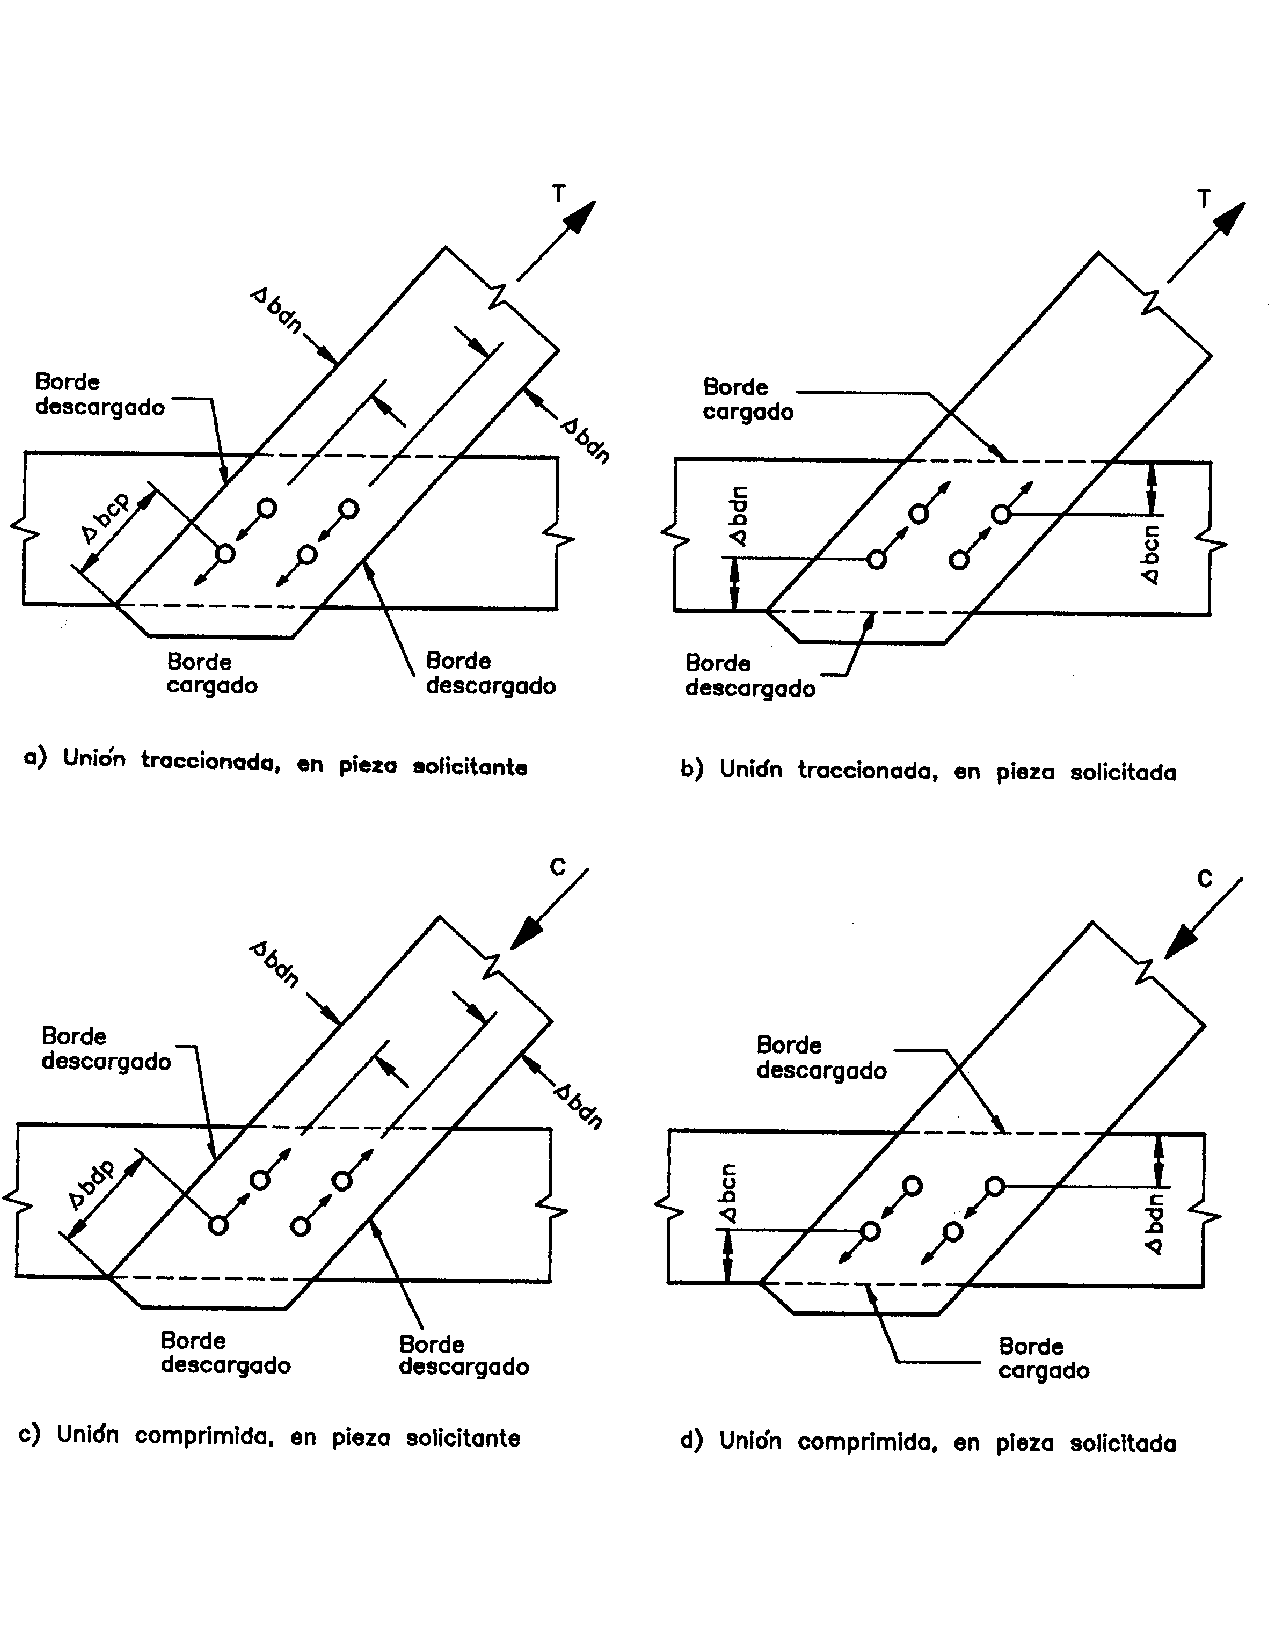
\includegraphics[width=1\linewidth]{Imagenes/figura_17.pdf}
\caption{Designaciones de espaciamientos y bordes. Fuente: NCh1198 - Madera - Construcciones en madera - Cálculo.}
\label{fig:nch_17}
\end{figure}

\newpage

\subsection{Verificaciones tensionales}
\subsubsection{Sección transversal neta}
La capacidad soportante de carga de las piezas debe verificarse en la menor sección transversal neta que condiciona la ejecución de las uniones, deduciendo de la sección transversal bruta las áreas de perforaciones o de cualquier otra remoción de madera.\\
Así, el área neta requerida en piezas traccionadas y comprimidas, se determina dividiendo la carga total que se traspasa a través de la sección transversal neta crítica, por los correspondientes valores de diseño $F_{tp,dis} $ o $F_{cp,dis}$. Para las solicitaciones donde existen elementos de unión alineados de forma alternada, estos se deben considerar dispuestos en una misma sección transversal, a excepción que el espaciamiento entre estos sea mayor o igual a:
\begin{itemize}
	\item 8 diámetros para pernos, barras de acero y tirafondos.
	\item 2 diámetros en caso de conectores.
\end{itemize}

\subsubsection{Tensiones de cizalle}
En uniones de pernos, barras de acero, tirafondos o conectores, solicitadas por fuerzas de corte, se debe verificar que las tensiones de cizalle de trabajo $f_{cz}$ no excedan los siguientes valores indicados:
\begin{itemize}
	\item En uniones separadas del extemo de la pieza, por una distancia $s_{bp}$ mayor o igual que 5 veces la altura de la misma: 
	\begin{equation}
		f_{cz} = \frac{3\cdot Q}{2\cdot b\cdot h_e} \leq 1,5\cdot F_{cz,dis}  
	\end{equation}
	\item En uniones separadas del extremo de la pieza, por una distancia $s_{bp}$ menor que 5 veces la altura de la misma:
	\begin{equation}
		f_{cz} = \frac{3Q}{2 b h_e} \frac{h}{h_e} \leq F_{cz,dis}
	\end{equation}
	\item Se debe verificar que la sección transversal bruta cumple con la relación:
	\begin{equation}
		f_{cz} = \frac{3\cdot Q}{2\cdot b\cdot h} \leq F_{cz,dis}
	\end{equation}		
\end{itemize}

Los valores $h$ y $h_e$ se muestran en la figura \ref{fig:nch_19}. El valor $h_e$ será distinto para conectores o para pernos, barras de acero y tirafondos. Para conectores $h_e$ corresponde a la altura de la pieza menos la distancia desde el borde descargado hasta el borde del conector más cercano, mientras que en el caso del resto de las uniones, se evalúa deduciendo de la altura, la distancia entre el borde descargado y el centro de la unión más próxima.

\begin{figure}[H]
\centering
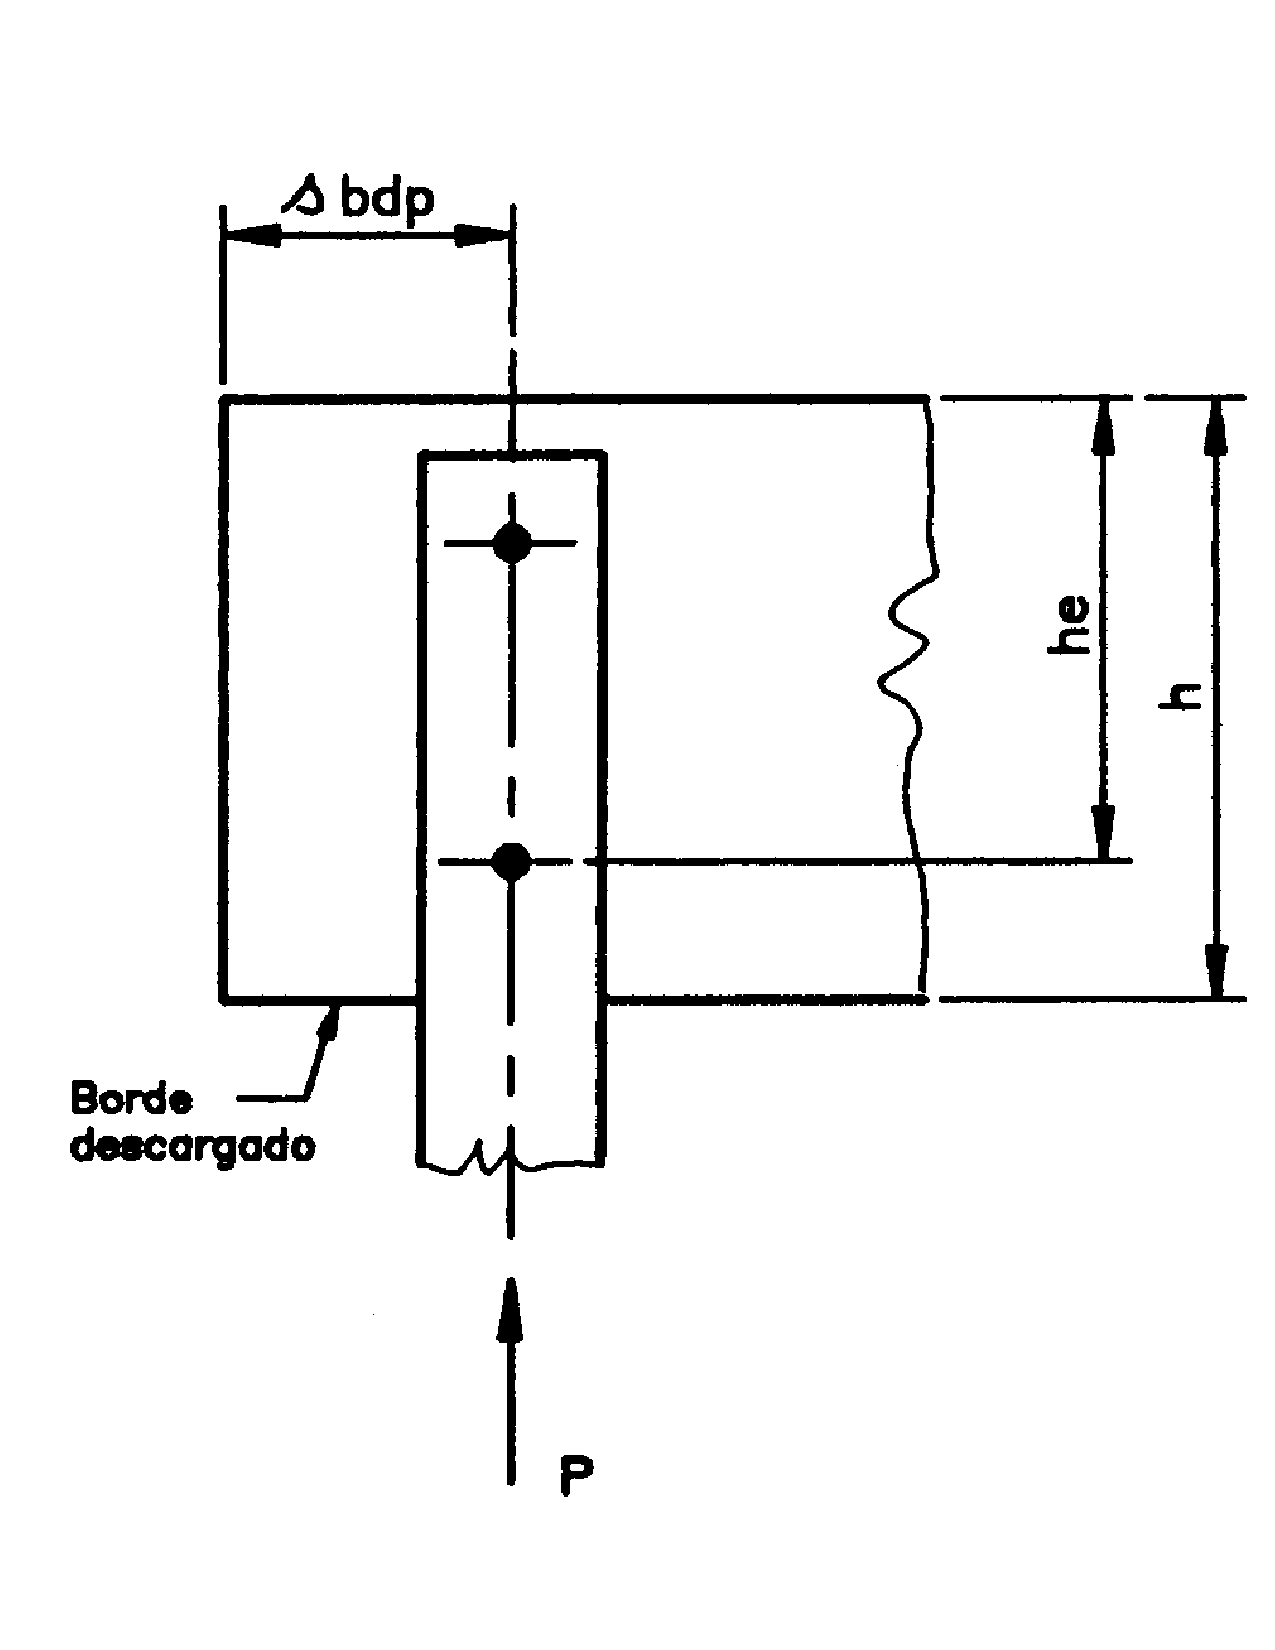
\includegraphics[width=0.45\linewidth]{Imagenes/figura_19.pdf}
\caption{Valor de $h_e$, para los distintos elementos de unión. Fuente: NCh1198 - Madera - Construcciones en madera - Cálculo.}
\label{fig:nch_19}
\end{figure}


\subsection{Número de elementos de unión}
Las cargas admisibles que se indican en esta norma, rigen para un elemento de unión individual, según las solicitaciones correspondientes. Una hilera de elementos de unión consiste en dos o más elementos del mismo tipo y tamaño alineados. En madera, es usual el uso de más de un elemento para unir dos o más maderas, debido a las restricciones existentes en su tamaño y distanciamiento.

\subsubsection{Carga admisible y factor de modificación por longitud de hilera}
La capacidad de carga admisible de una hilera es la suma de las capacidades de cada elemento que constituye la unión, sin embargo, no debe sobrepasar el valor $P_h$, determinado por la ecuación \ref{eq:adm_hilera}.

\begin{equation}\label{eq:adm_hilera}
	P_h = K_u \cdot \sum P_i
\end{equation}
Donde $\sum P_i$ es la suma de los valores admisibles de los elementos de unión individuales existentes en la hilera y $K_u$ es el factor de modificación por longitud de hilera, señalado en la sección \textbf{10.3.2.2} y las tablas 30 y 31 de la norma.

\subsection{Uniones con perno}
\label{sec:union_perno}
Las especificaciones para pernos son aplicables para cualquier elemento cilíndrico de acero que atreviese perpendicularmente los planos de cizalle de la unión y que quedan solicitados preponderantemente en flexión induciendo sobre la madera tensiones de aplastamiento.

Para su correcta instalación es necesario que los agujeros y las arandelas cumplan con ciertas dimensiones. El diámetro del agujero se debe mayorar respecto al del perno en función del tamaño del perno y las condiciones de humedad de servicio, siguiendo la tabla 33 de la sección \textbf{10.5.1.2} de la norma. Para las arandelas o golillas, se debe seleccionar primero si se utilizará una de forma circular o cuadrada, dando preferencia a esta última por ofrecer mayor resistencia al incrustramiento en la madera. Luego , sus respectivas dimensiones están en función del diámetro del perno, siguiendo la tabla 34 de la norma.

Respecto a las características del perno, su diámetro nominal debe estar entre los 10 y 30 mm. Además, se exige una disposición mínima de dos pernos, exceptuando los casos donde un único perno no queda solicitado en un porcentaje superior al 50\% de su capacidad de diseño.

\subsubsection{Cargas admisibles para un perno}
Las cargas admisibles para este tipo de unión solo son aplicables cuando la dirección de la solicitación es perpendicular a su eje para duración normal y de madera seca que permanecerá seca en servicio. Para casos distintos es necesario aplicar los factores de modificación correspondientes. Por otro lado, en esta norma existen condiciones distintas para cizalle simple, doble o múltiple, sin embargo, cizalle simple y múltiple se calculan realizando modificaciones al cizalle doble, por lo tanto, sólo se efectuara una explicación de este caso.

La capacidad de carga admisible ($P_{ad}$) se calcula estableciendo que la unión está establecida por la unión de tres piezas de la misma especia, con las piezas laterales paralelas entre sí y cada una de ellas de espesor igual a la mitad del espesor de la pieza central, e, como se muestra en la figura \ref{fig:nch_23}. Así, es posible obtenerla a través de la tensión admisible de aplastamiento nominal ,$F_{ap}$ (\ref{eq:f_ap}) , la esbeltez de la unión $\lambda_u$ y el diámetro del perno ($D$), de acuerdo a la siguiente expresión:
\begin{equation} \label{eq:padm_ad}
	P_{ad} = F_{ap} \cdot \lambda_u \cdot D^2 \leq Z \cdot D^2
\end{equation}

Y la tensión admisible de aplastamiento nominal se define como:
\begin{equation}\label{eq:f_ap}
	F_{ap} = \frac{0,00065\cdot \rho_{12,k}\cdot (100 - D)}{\eta (2,75\cdot \sin^2(\theta) + \cos^2(\theta)} \qquad \text{(MPa)}
\end{equation}


Donde:
\begin{align*}
&\rho_{12,k} &: \qquad &\text{Es la densidad normal característica de la especie forestal, en kg/m}^3 \text{, según}\\
& & & \text{tabla E2 del anexo E de la norma. D es el diámetro del perno, en mm.}\\
&D &: \qquad &\text{Diámetro del perno, en mm}\\
&\eta &: \qquad &\text{Es el factor de reducción de la zona elástica, según tabla 35 de la norma.}\\
&\theta &: \qquad &\text{Es la desangulación fuerza-fibra.}\\
&\lambda_u = \frac{e}{D} &: \qquad &\text{Esbeltez del perno en la pieza central}\\
&Z &= \qquad &1,15\cdot \sqrt{\frac{F_{ap} \cdot F_y}{\eta}} \qquad \text{(MPa)}\\
&F_y &: \qquad &\text{Tensión de fluencia del acero, usando 240 MPa como referencia} 
\end{align*}

\begin{figure}[H]
\centering
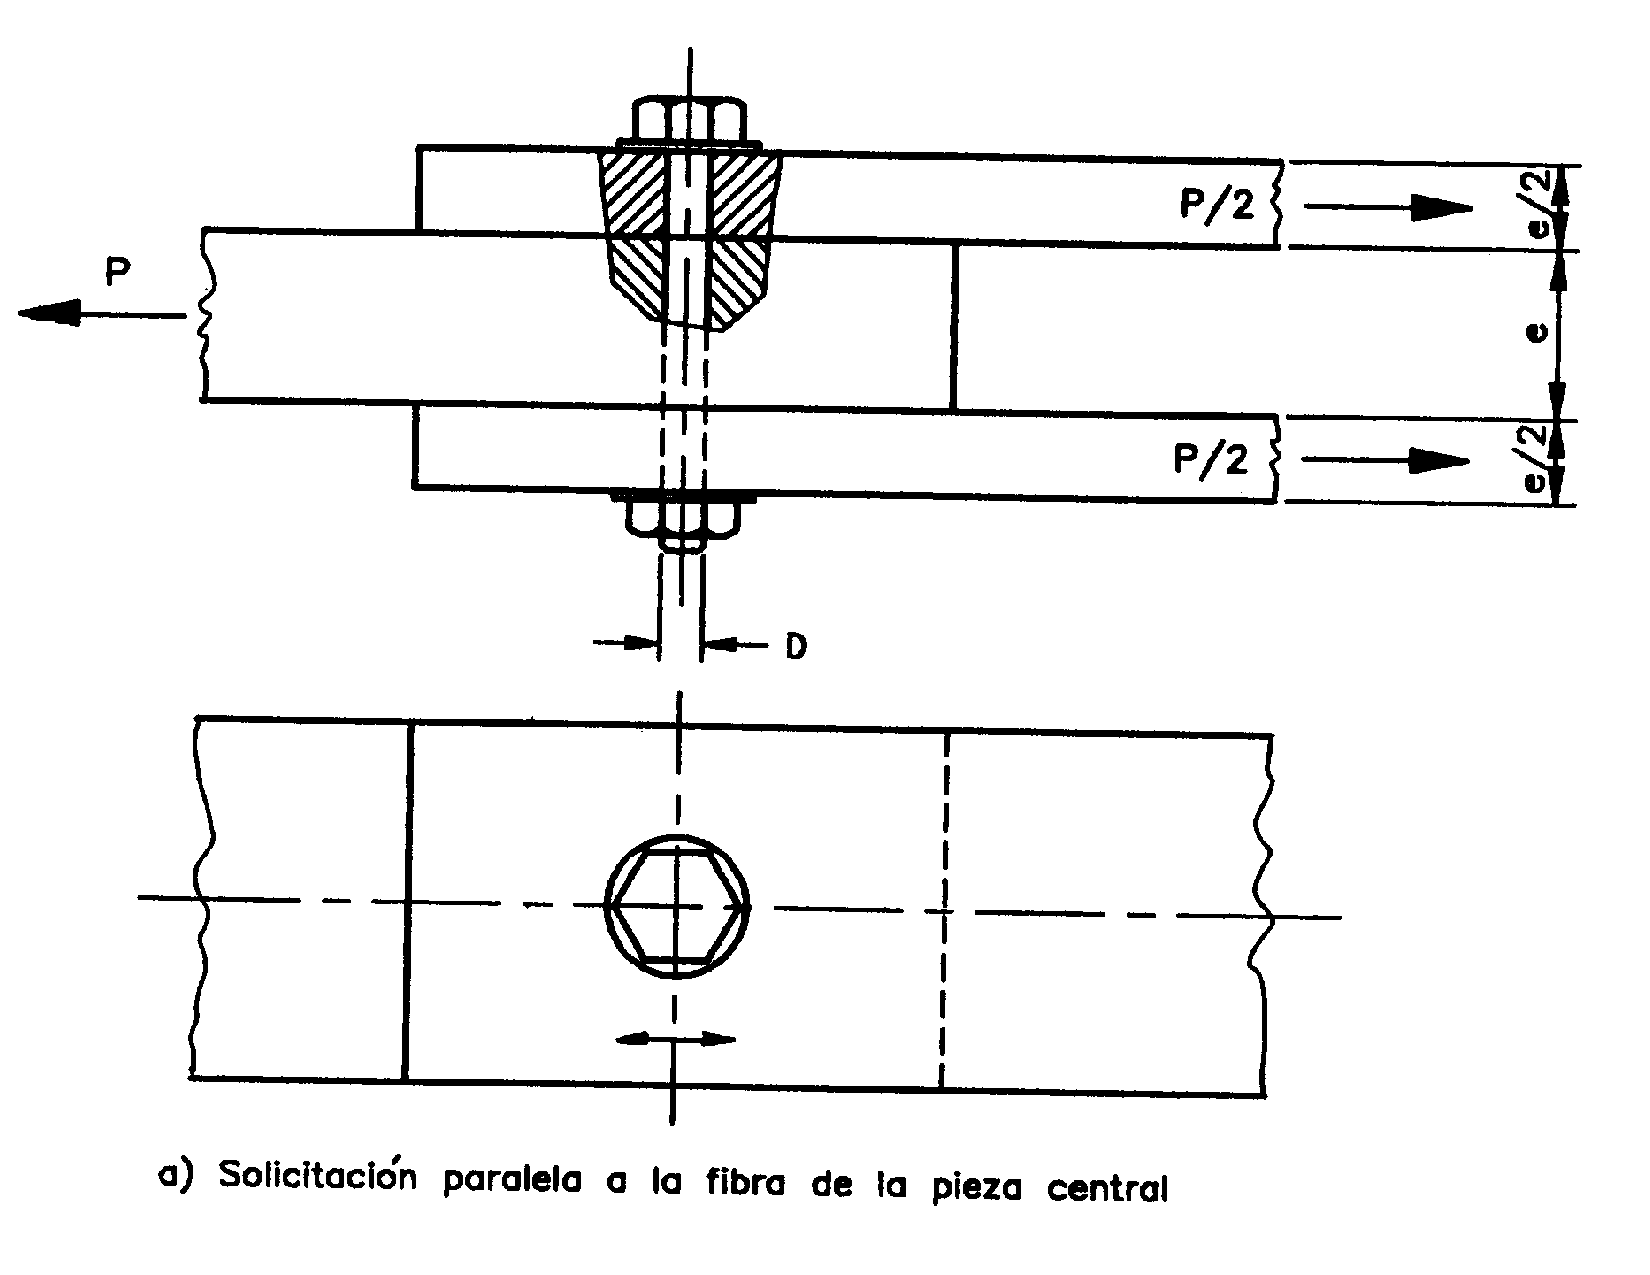
\includegraphics[width=0.5\linewidth]{Imagenes/figura_23A.pdf}%
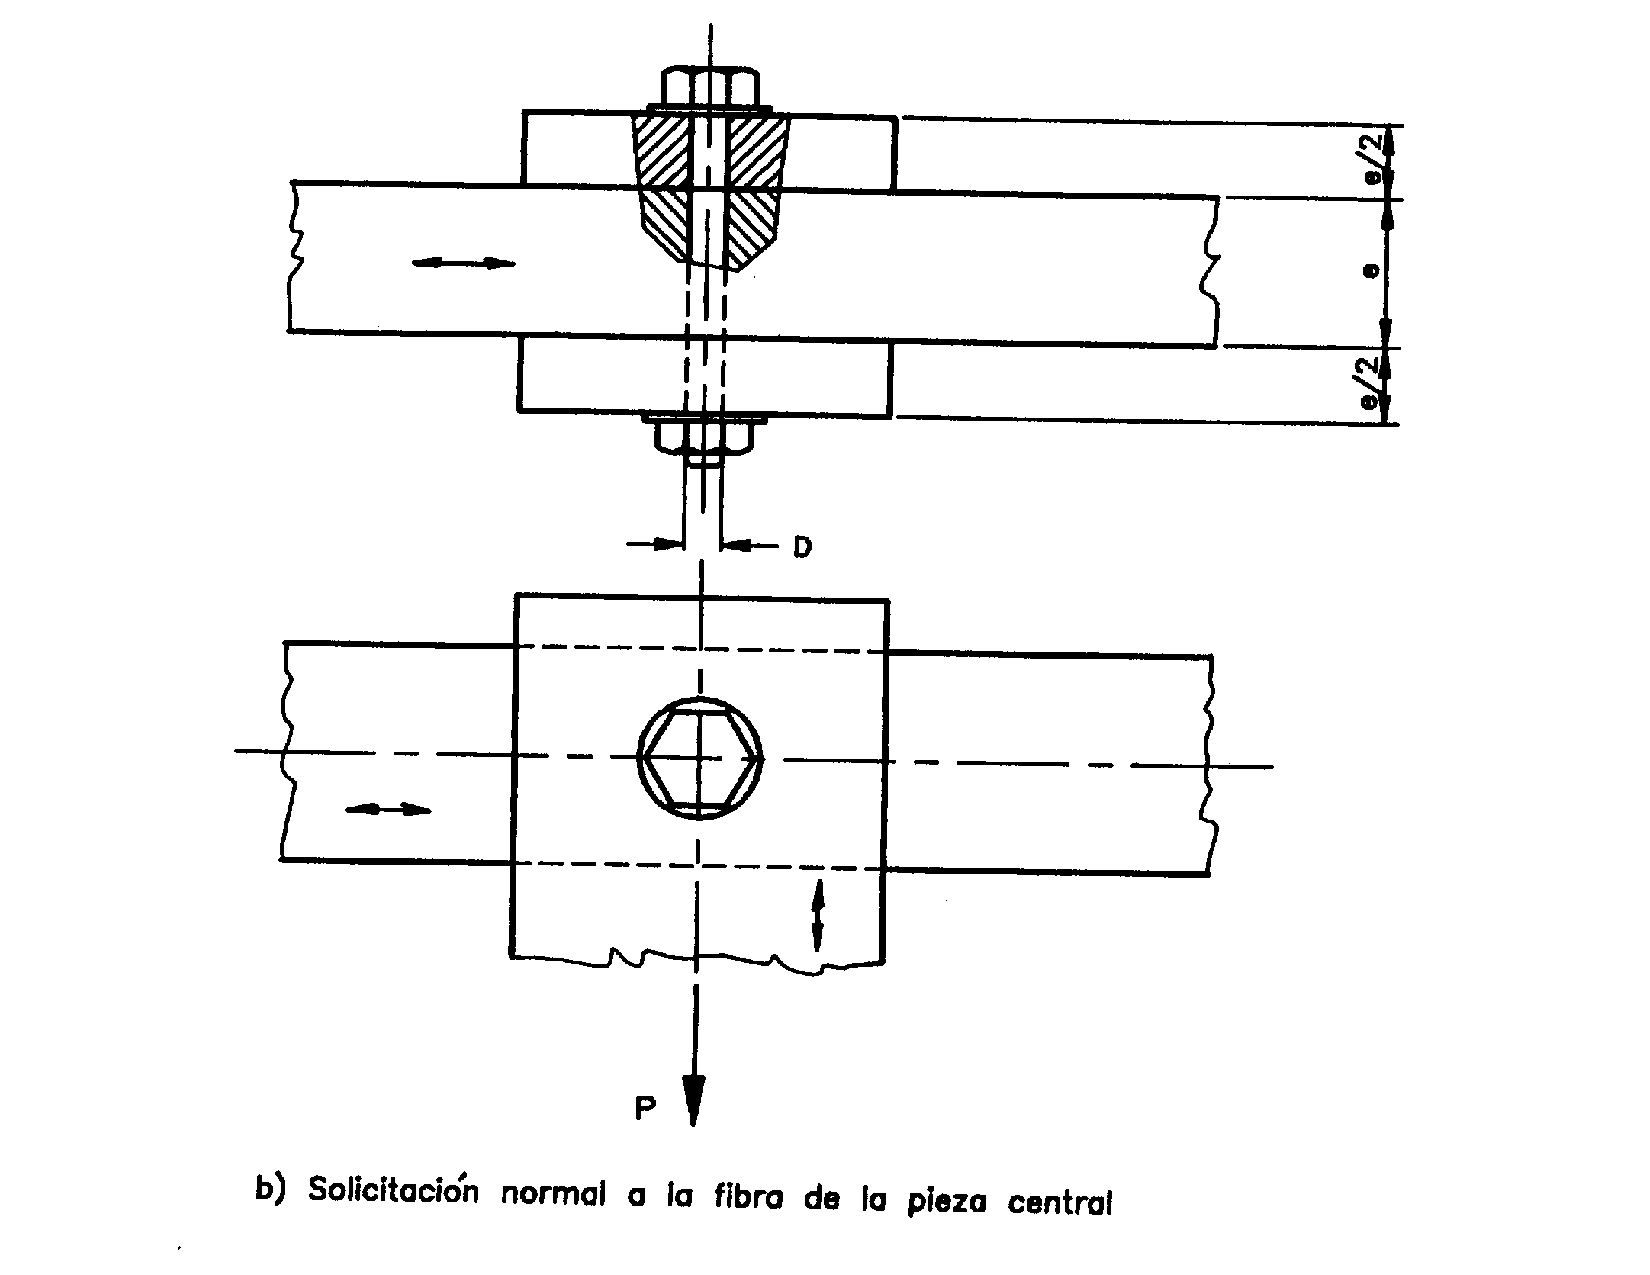
\includegraphics[width=0.5\linewidth]{Imagenes/figura_23B.pdf}
\caption{Uniones en cizalle doble. Fuente: NCh1198 - Madera - Construcciones en madera - Cálculo.}
\label{fig:nch_23}
\end{figure}


Para casos distintos al establecido anteriormente, se deben realizar arreglos en la forma de cálcular $P_{ad}$. En caso que las piezas laterales tengan un espesor menor que la mitad del espesor de la pieza central $e$, la carga admisibles es igual a la de una unión de cizalle doble con una pieza central de espesor ficticio, $e*$, equivalente al doble del espesor de la pieza lateral más delgada. Si las piezas laterales están constituidas de una especie maderera distinta a la pieza central, se debe considerar la menor entre:
\begin{itemize*}
	\item El valor determinado para una unión equivalente con todas sus piezas de la especie usada en las piezas laterales.
	\item El valor determinado para una unión equivalente con todas sus piezas constituidas con la especie de la pieza central.
\end{itemize*}

Cuando se usen planchas de acero como piezas laterales, las cargas admisibles para solicitaciones orientadas según la dirección de la fibra, se pueden mayorar en un 25\%, sin embargo estas mayoraciones no se permiten para las cargas admisibles calculadas con solicitaciones normales a la fibra.

El valor obtenido de $P_{ad}$ según la ecuación \ref{eq:padm_ad}, considera el eventual aflojamiento de tuercas inherentes a la contracción de la madera.

Finalmente, para cizalle simple existen dos casos a considerar. Cuando la unión está constituida por dos piezas de espesores diferentes, la carga admisible se determina como el menor valor entre:
\begin{itemize*}
	\item La mitad de la carga admisible de una unión de cizalle doble con una pieza central de espesor igual al de la pieza más gruesa.
	\item La mitad de la carga admisible de una unión de cizalle doble con una pieza central de espesor igual al doble del espesor de la pieza más delgada.
\end{itemize*}
El segundo caso, cuando las piezas son de igual espesor, la carga admisible equivale a la mitad de la correspondiente a la de una unión de cizalle doble con una pieza central de espsor igual al de cada pieza.

\subsubsection{Espaciamientos mínimos para pernos}
\label{sec:espaciamiento_pernos}
Los espaciamientos mínimos que se deben respetar en las uniones con pernos se esquematizan en la figura \ref{fig:nch_26}. El espaciamiento mínimo entre los pernos y los bordes cargados o descargados se establecen en función del diámetro del mismo, determinados por la tabla 36 de la sección \textbf{10.5.4} de la norma. El espaciamiento mínimo ente los pernos mismos, se establecen en la tabla 37 de la misma sección. 

\newpage

\begin{figure}[H]
\centering
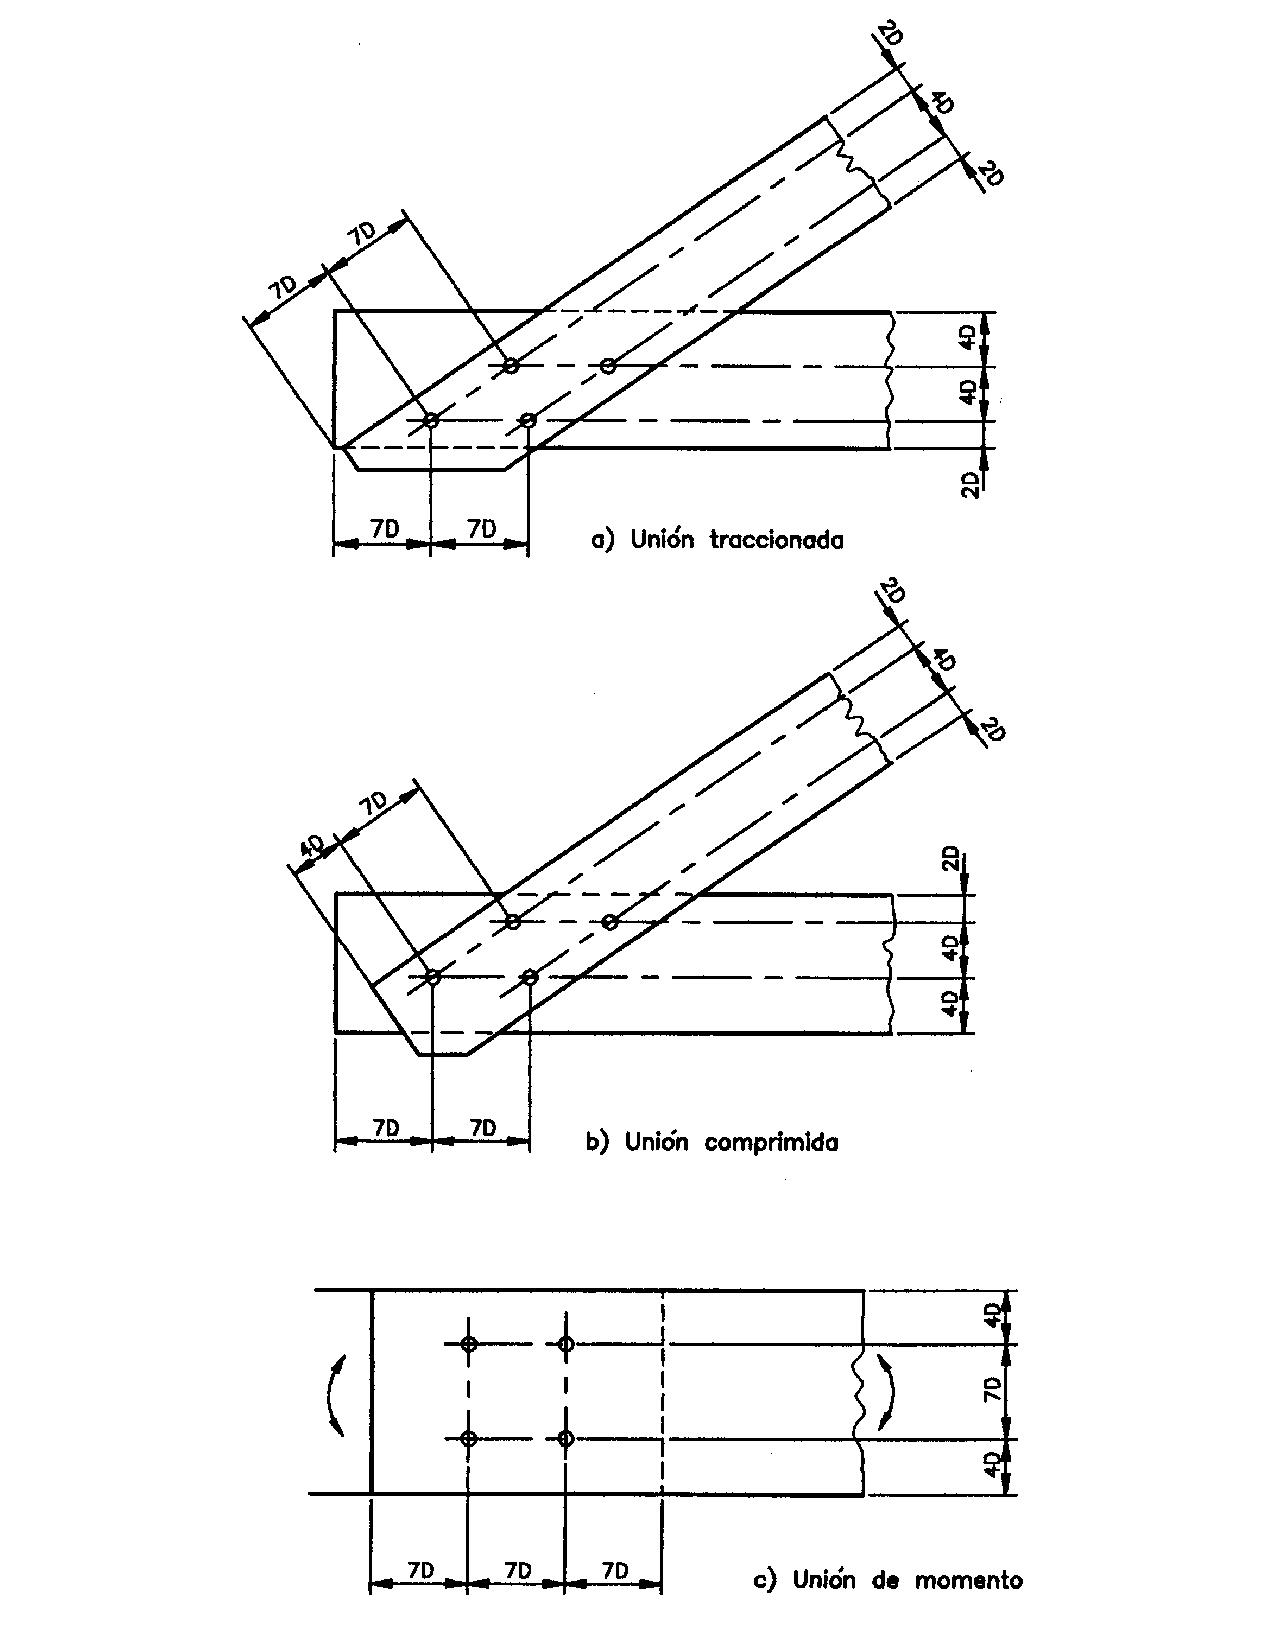
\includegraphics[width=1\linewidth]{Imagenes/figura_26.pdf}%
\caption{Espaciamientos mínimos ntre pernos, barras de acero, tirafondos y a los bordes. Fuente: NCh1198 - Madera - Construcciones en madera - Cálculo.}
\label{fig:nch_26}
\end{figure}

\subsection{Uniones con tirafondos}
\label{sec:tirafondos}
Los tirafondos son un tipo de unión mecánica similar a un tornillo, del cual se diferencia porque su longitud total está dividida en una zona roscada y otra lisa llamada vástago, como se muestra en la figura \ref{fig:nch_28}. Las especificaciones y cálculos indicado en esta norma son válidos para tirafondos que cumplan con las características del anexo M de la norma.

Para obtener los valores de diseño para este tipo de unión, es necesario clasificar las especies madereras utilizadas según su densidad anhidra $\rho_o$ (obtenidas en el anexo E), de acuerdo a la tabla 38 de la norma.

\begin{figure}[H]
\centering
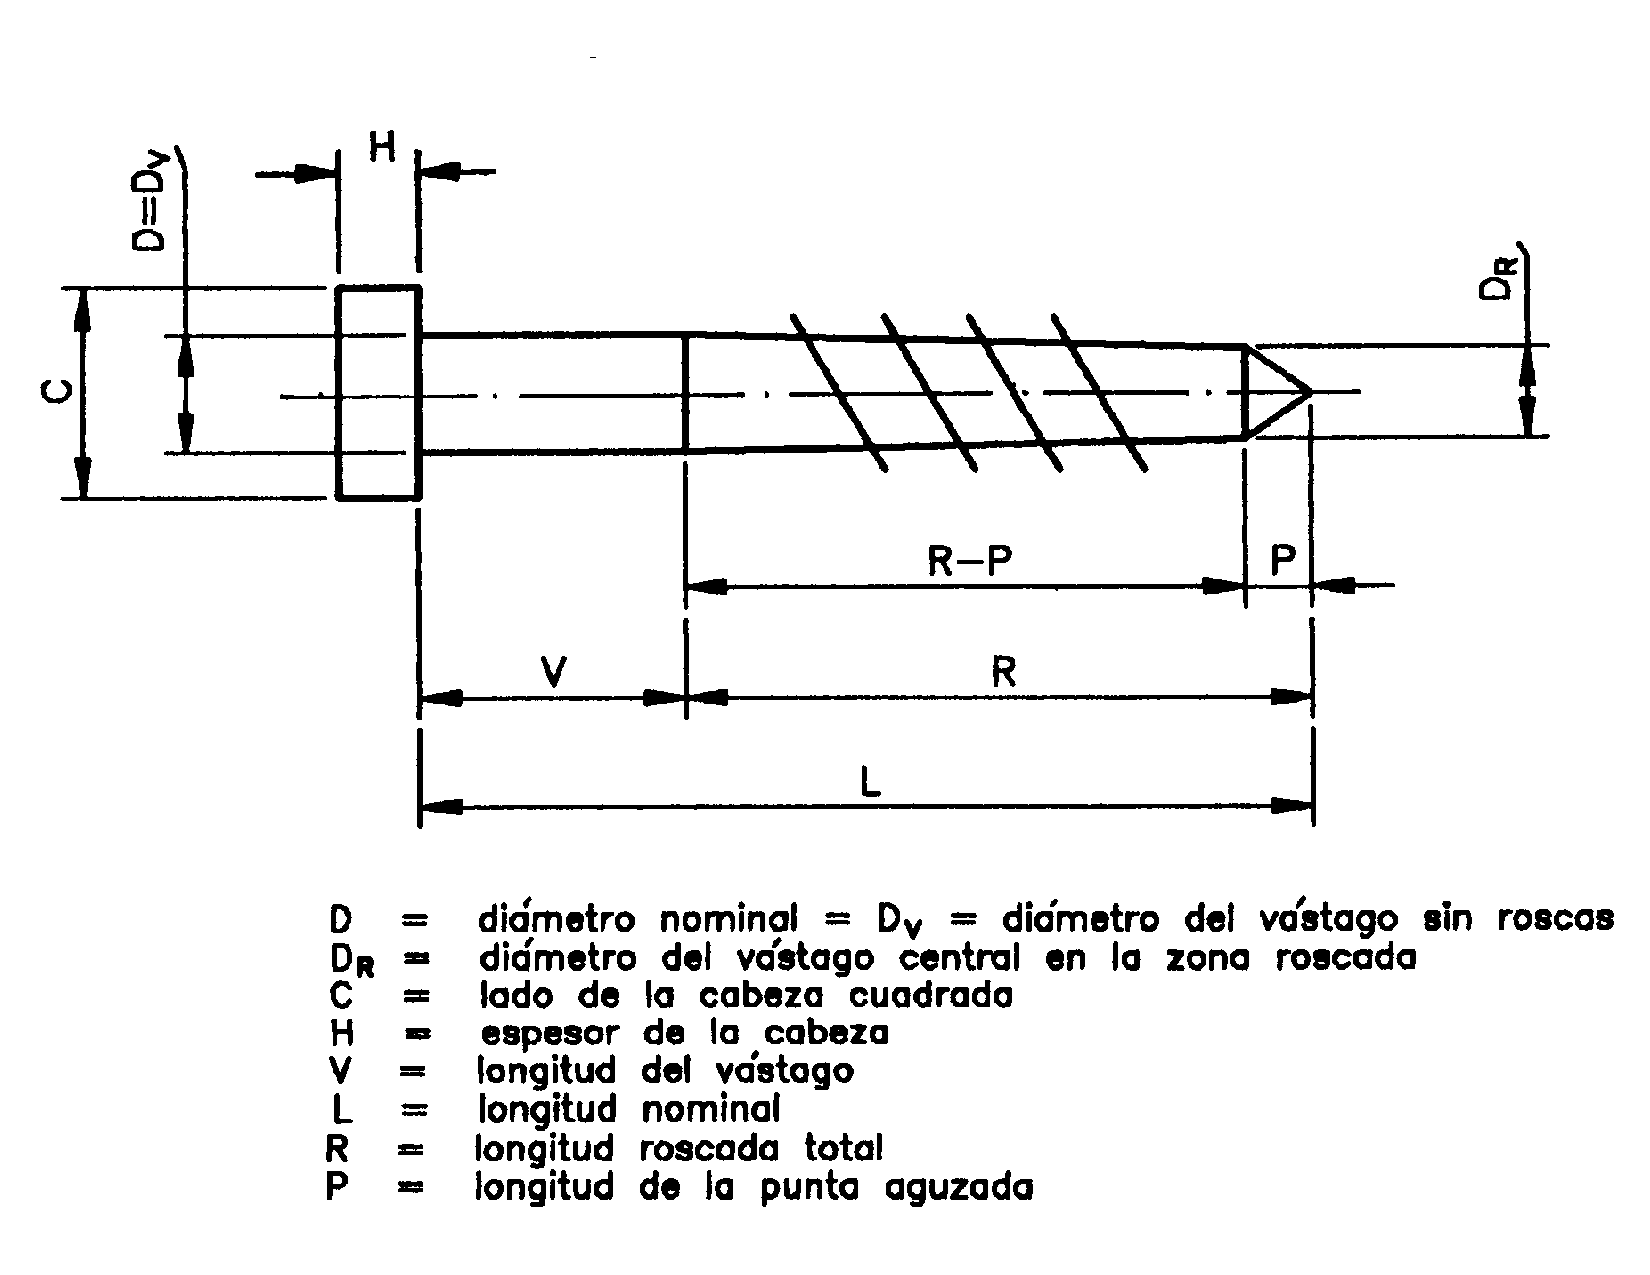
\includegraphics[width=0.9\linewidth]{Imagenes/figura_28.pdf}%
\caption{Esquema de un tirafondo. Fuente: NCh1198 - Madera - Construcciones en madera - Cálculo.}
\label{fig:nch_28}
\end{figure}

\subsubsection{Perforaciones guía}
Los tirafondos deben ser instalados en perforaciones guías con las características siguientes:
\begin{itemize*}
	\item El agujero en donde se alojará el vástago del tirafondo debe tener el mismo diámetro $D$ de dicho vástago y una profundidad igual a la longitud, $V$, de la zona sin rosca del tirafondo.
	\item El agujero para la zona con rosca del tirafondo debe tener una profundidad de al menos igual a la longitud de la zona roscada del tirafondo, $R-P$ y un diámetro comprendido entre:
	\begin{itemize*}
		\item 40\% - 70\% del diámetro del vástago para las especies del grupo A de la tabla 38 de la norma.
		\item 60\% - 75\% de dicho diámetro para las especies del grupo B.
		\item 65\% - 85\% para las de los grupos C y D.
	\end{itemize*}
\end{itemize*}
Para tirafondos de diámetros iguales o mayores que $3/4"$ (ver anexo M) ocupar los porcentajes del límite superior de los intervalos señalados. Cuando los tirafondos con diámetros menores o iguales a $3/8"$ colocados en maderas del grupo A y B son sometidos a extracción directa, se puede evitar la perforación guía si los espaciamientos entre tirafondos y las distancias a los bordes de la pieza cumplen con las seccionas \textbf{10.5.4.1} y \textbf{10.5.4.2}.
La zona con rosca debe ser colocada en la perforación guía con una llave de tuerca. Se prohibe la aplicación de golpes de martillo en esta operación. Para facilitar la introducción y evitar daños en el tirafondo se acepta el empleo de lubricantes en la rosca o en la perforación.

\subsubsection{Arandelas}
Las arandelas siguien las especificaciones de la tabla 34 de la norma, señaladas en la sección de la unión con pernos, excepto que se dipongan planchas de acero.

\subsubsection{Solicitaciones de extracción lateral}
La carga admisible de extracción lateral de tirafondos colocados en su eje normal a las fibras de la madera y sometidos a una carga paralela a dichas fibras, se obtiene a partir de la siguiente expresión:
\begin{equation}\label{eq:pel_ad}
	P_{el,ad}=K\cdot D^2 \cdot 10^{-3} \qquad \text{(kN)}
\end{equation}
Donde $P_{el,ad}$ es la carga admisible de extracción lateral, $D$ el diámetro del vástago del tirafondo, en mm, y $K$ es la constante que depende de la densidad anhidra y cuyo valor se puede obtener de la tabla 39 de la norma.
Las cargas admisibles son aplicables sólo si se cumplen las siguientes condiciones:
\begin{enumerate}
	\item El espesor $e_L$ de la pieza lateral atravesada por el tirafondo es igual a $3,5D$.
	\item La profundidad mínima de penetración en la pieza principal (la que recibe la punta del tirafondo), asciende a:
	\begin{itemize}
		\item $7D$ en maderas de los grupos C y D.
		\item $11D$ en maderas de los grupos A y B.
	\end{itemize}
	\item La penetración del vástago es completa en la pieza lateral, sin que él penetre en la pieza principal, como se muestra en la figura 29 de la norma. 
\end{enumerate}

En caso de no cumplirse las condiciones señaladas, es necesario multiplicas el valor $P_{el,ad}$ obtenido en la ecuación \ref{eq:pel_ad} por los factores de modificación correspondientes.
\begin{enumerate}
	\item \textbf{Factor de modificación por espesor de la pieza lateral, $K_{te}$}\\
	Para espesores de piezas laterales diferentes a $3,5D$, se debe utilizar la tabla 40 de la norma.
	\item \textbf{Factor de modificación por penetración del vástago en la pieza principal, $K_{tv}$}\\
	Cuando el vástago toca la pieza principal, se debe utilizar el factor de modificación señalado en la tabla 41 de la norma, utilizando la razón $P_v / D$ como dato de entrada, donde $P_v$ se especifica en la figura 30 de la norma.	
\end{enumerate}

Además, siempre se debe multiplicar la carga admisible a la extracción lateral de la ecuación \ref{eq:pel_ad} por el factor de modificación por diámetro, $K_{tD}$, que se entrega en la tabla 42 de la norma.

Cuando $P_{el,ad}$ es calculado para tirafondos colocados con su eje paralelo a las fibras de la madera de la pieza principal y sometidos a una carga normal a dichas fibras se debe considerar igual a $2/3$ de la multiplicación de $P_{el,ad} \cdot K_{tD}$. Por otro lado, cuando se usen cubrejuntas metálicas, la carga admisible de extracción lateral se debe amplificar en un 25\% para cargas paralelas de la dirección de la fibra. Esta mayoración no se aplica sobre la carga admisible normal a la dirección de la fibra.

\subsubsection{Solicitaciones de extracción directa}
La carga admisible de extracción directa de tirafondos colocados con su eje normal a las fibras de la madera, se determina con la expresión:
\begin{equation}\label{eq:ped_ad}
	P_{ed,ad} = \frac{\rho_{o}^{1,5} \cdot D^{0,75} \cdot l_{crit}}{978} \cdot 10^{-3} \qquad \text{(kN)}
\end{equation}
Donde:

\begin{align*}
&P_{ed,ad} &= \quad &\text{carga admisible de extracción directa}\\
&\rho_o &= \quad &\text{Densidad anhidra de la madera en} kg/m^3 \\
&D &= \quad &\text{Diámetro del vástago del tirafondo en mm}\\
&l &= \quad &\text{Longitud de penetración de la zona roscada del tirafondo (R-P) en la madera, en mm}\\
&l_{crit} &= \quad &\text{Longitud de penetración de la zona roscada que desarrolla la capacidad admisible de}\\
& & & \text{tracción  en la sección transversal crítica del tirafondo, según tabla 43 de la norma.}
\end{align*}

En caso que la solicitación de la extracción directa quede con su eje colocado paralelo a las fibras de la madera, se debe considerar una carga admisible igual al 75\% de aquella calculada para tirafondos colocados con su eje normal a las fibras de la madera.

\subsubsection{Combinación de solicitaciones de extracción directa y lateral}
Cuando un tirafondo esté solicitado tanto en extracción directa como lateral, el análisis se realiza por separado, no debiendo exceder la carga de diseño de extracción para ninguno de los dos casos.

\subsubsection{Espaciamiento}
Las distancias entre tirafondos y entre tirafondos y bordes debe seguir lo establecido en la tabla 36 del capítulo de pernos de la norma, donde se reemplaza el diámetro del perno por el diámetro del vástago.

%%Apendice B
%
\chapter{Tablas de carga de la máquina de fatiga}
\label{ch:anexo_b}

\section{Tabla de cargas original}
\label{sec:anexob1}

La siguiente tabla es la que se utiliza actualmente para realizar los ensayos de fatiga en flexión. Se muestra en sus unidades y orden original.

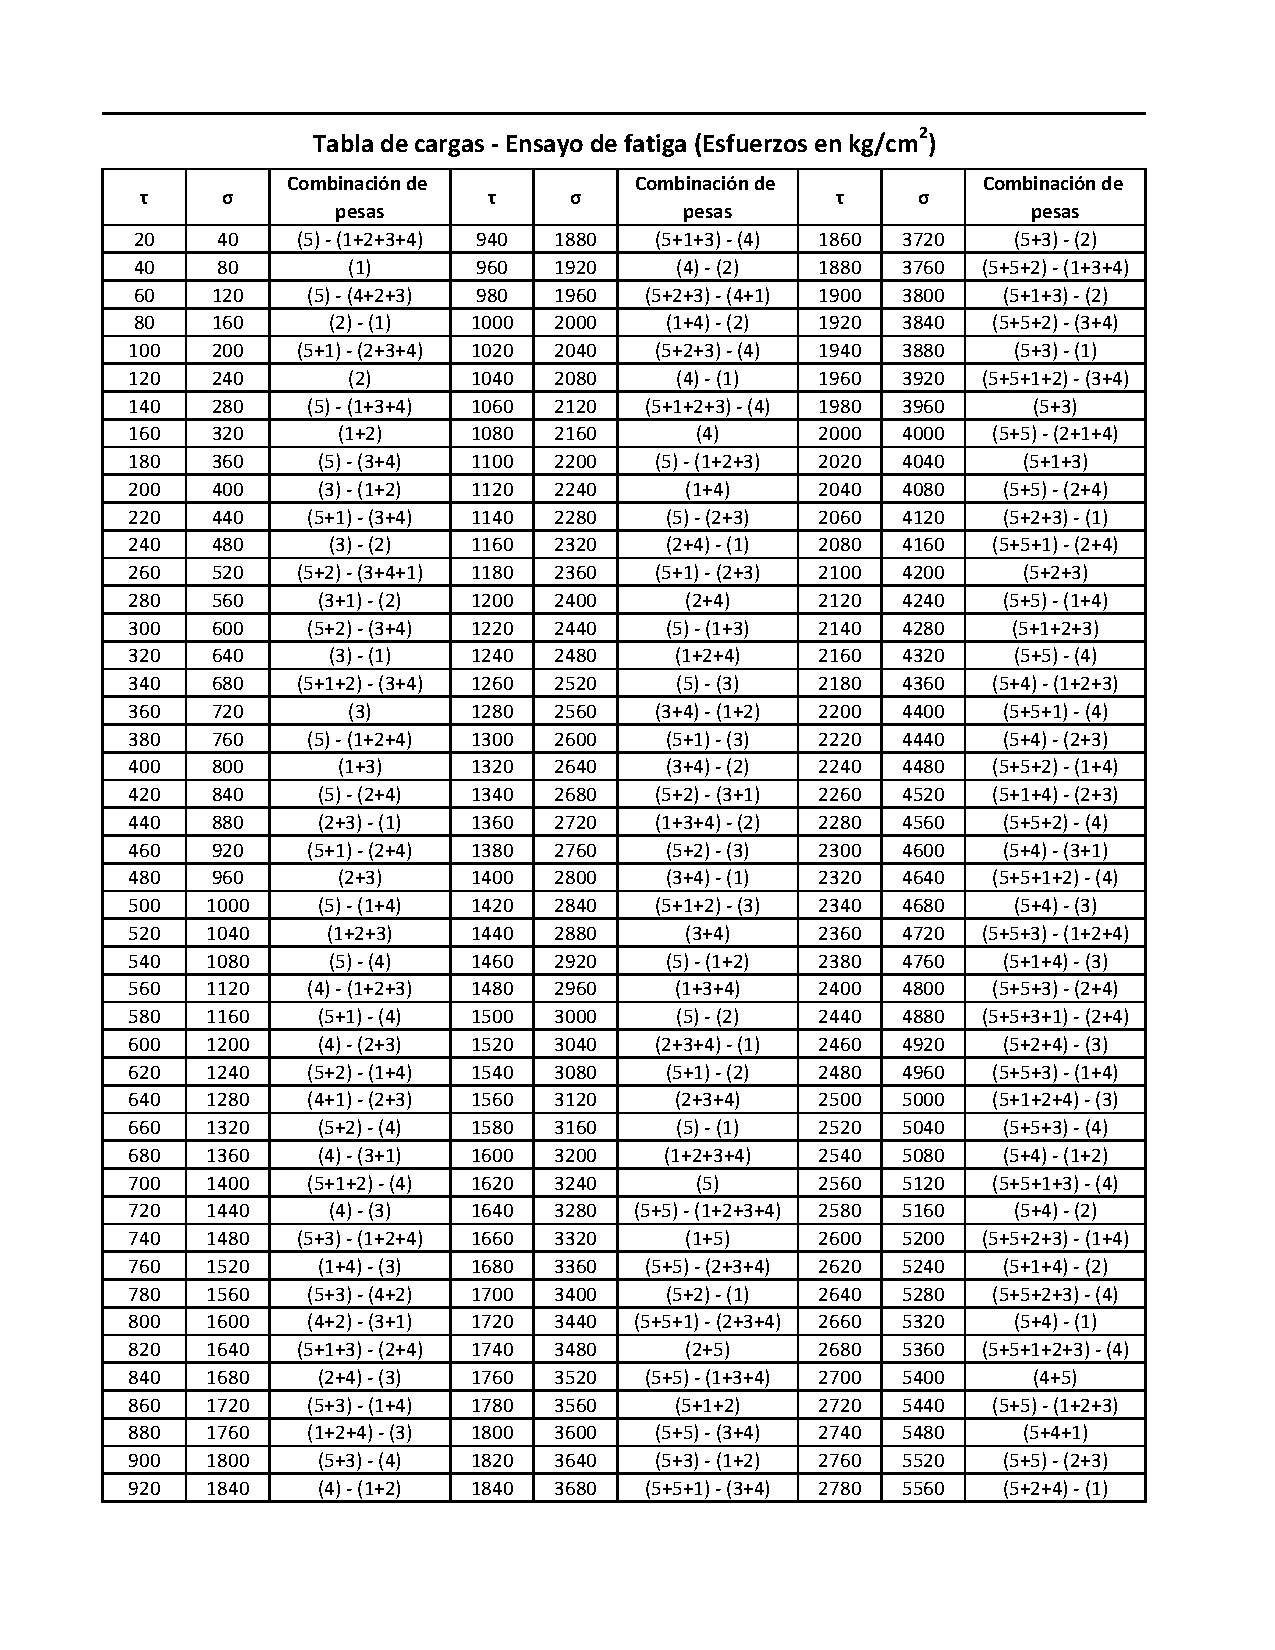
\includepdf[pages=-]{Anexos/anexo_b1.pdf}

\section{Tabla de cargas propuesta}
\label{sec:anexob2}

Esta nueva tabla es la propuesta que emana de los resultados del trabajo realizado. Los esfuerzos de cortante máximo y de von Mises se toman a partir del punto $P$, según la fig. \ref{fig:diag_pqr}. Además, se añade la columna  $F_{max}$ que corresponde a la carga máxima obtenida en el modelo dinámico del sistema para cada combinación de contrapesos.

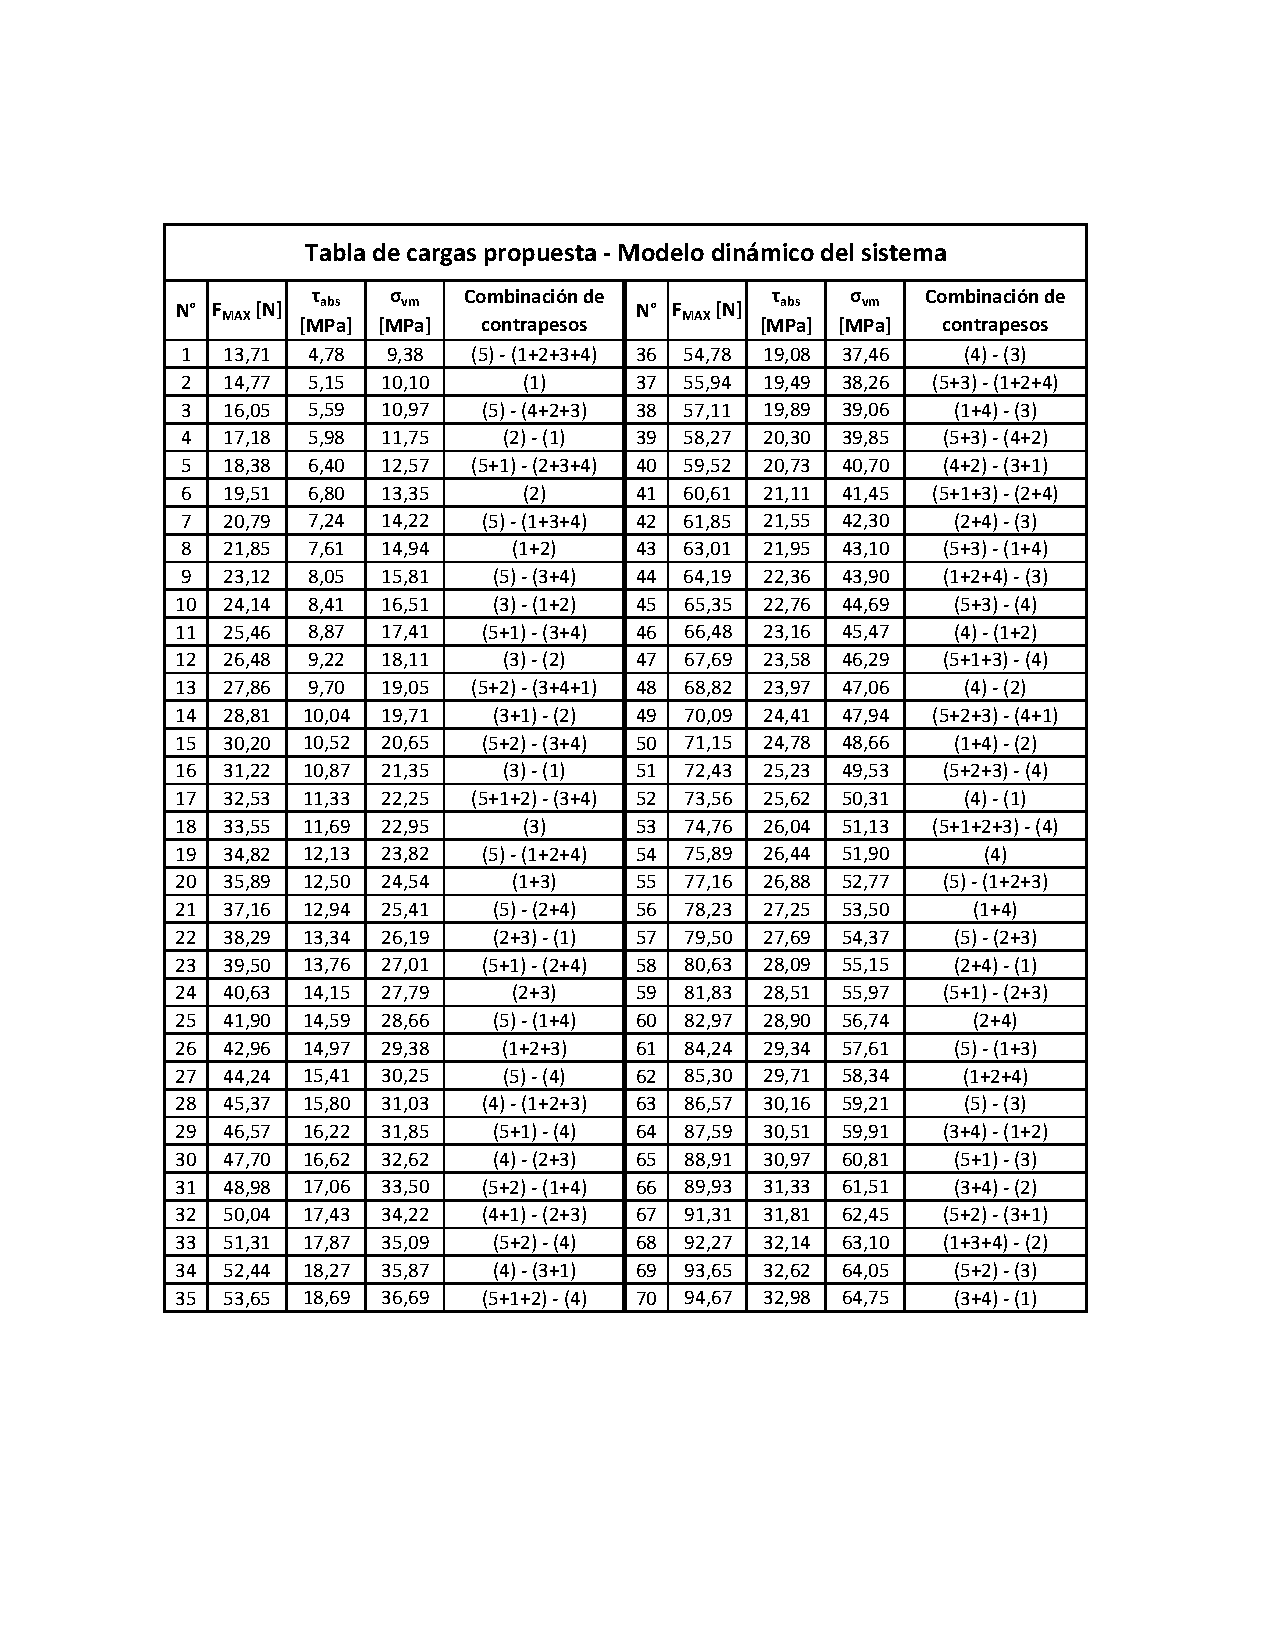
\includepdf[pages=-]{Anexos/anexo_b2.pdf}

\section{Tabla de cargas de la simulación elasto-plástica}
\label{sec:anexob3}

Tabla de las 76 cargas utilizadas para buscar el esfuerzo de fluencia y el esfuerzo último de la probeta. La columna $F_{max}$ corresponde a las cargas aplicadas sobre la probeta. Las columnas $\tau_{max}$ y $\sigma_{vm}$ son los resultados obtenidos para cada nivel de carga. Finalmente, $\Delta m$ es el contrapeso necesario en la máquina para aplicar la carga respectiva, calculada mediante la ec. \ref{eq:deltam}.

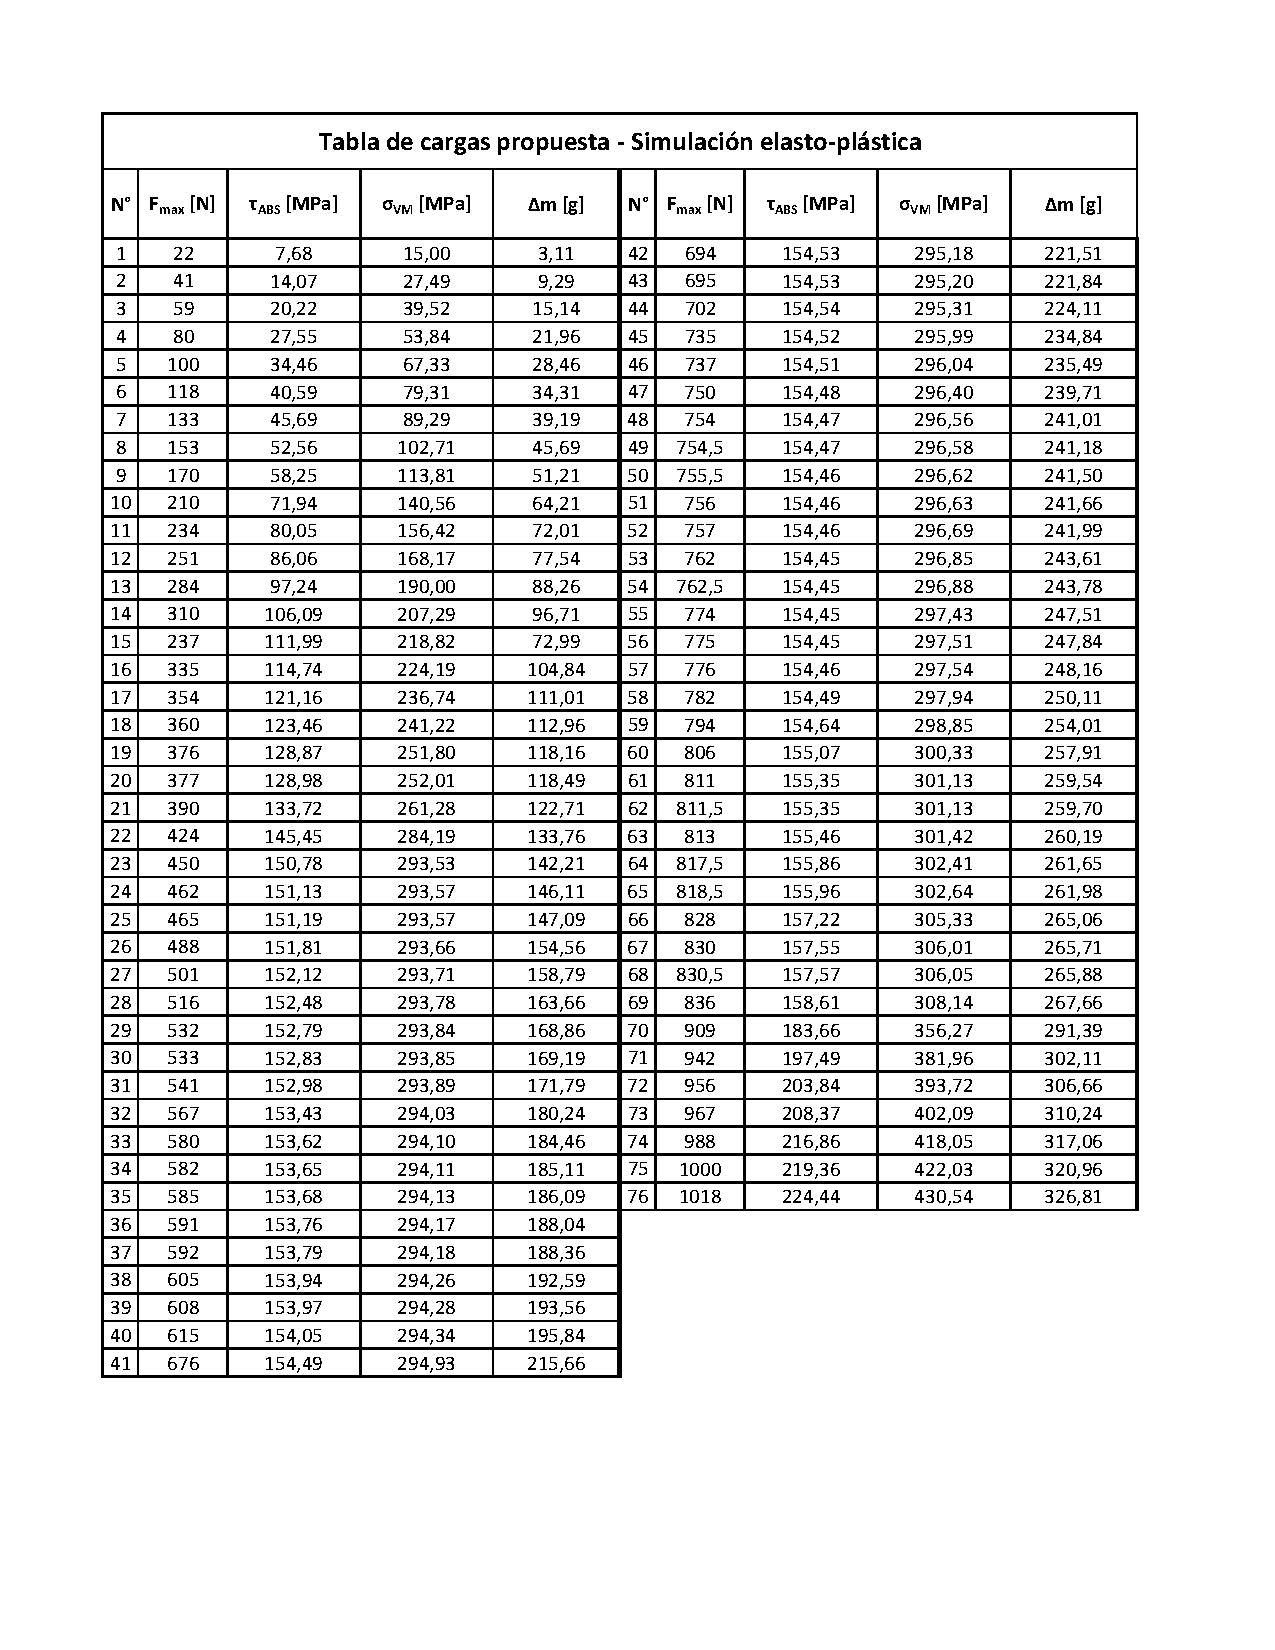
\includepdf[pages=-]{Anexos/anexo_b3.pdf}
%

%%% Incluir la bibliograf'ia. Mirar el archivo "biblio.bib" para m'as detales
%%% y un ejemplo.
%

\nocite{*}     %incluir en la bibliografia articulos no citados
\bibliography{Bibliografia/biblio}
\end{document}
